
\documentclass[12pt,a4paper]{report}

% ---------- PACKAGES ----------

\usepackage[utf8]{inputenc}
\usepackage{lmodern}
\usepackage{microtype}
\usepackage[T1]{fontenc}
\usepackage{graphicx}
\usepackage{setspace}
\usepackage{geometry}
\usepackage{titlesec}
\usepackage{tocloft}
\usepackage{fancyhdr}
\usepackage{hyperref}
\usepackage{caption}
\usepackage{textcomp}
\usepackage{booktabs}
\usepackage{longtable}
\usepackage{enumitem}
\usepackage{siunitx}

\usepackage{tikz}
\usetikzlibrary{shapes, arrows.meta, positioning, decorations.pathmorphing}
\usepackage{array}
\usepackage{booktabs}
\usepackage{circuitikz}
\onehalfspacing

\usepackage[fleqn]{amsmath}
\usepackage{amssymb}
\usepackage{float}
\usepackage{geometry}
\geometry{a4paper, margin=1in}
\usepackage{titlesec}
\usepackage{setspace}
\usepackage{pgfgantt}
\usepackage{hyperref}
\hypersetup{
	pdftitle={Your Title},
	pdfauthor={Your Name}
}
\onehalfspacing
\setlength{\mathindent}{0pt}
\setlength{\parskip}{0.5em}

\usepackage{tabularx}
\usepackage{booktabs}
\usepackage{longtable}
\usepackage{tabularx}
\usepackage{array}
\usepackage{booktabs}

% ---------- PAGE SETTINGS ----------
\geometry{
	left=1.25in,
	right=1in,
	top=1in,
	bottom=1in,
	headheight=15pt
}

\hypersetup{
	colorlinks=true,
	linkcolor=black,
	citecolor=black,
	urlcolor=blue,
	pdftitle={Design \& Development of Dual Band Directional Jamming System},
	pdfauthor={Rameen Khan, Mohammad Hasnain Abbasi, Mahroona Mariam Khan}
}
\makeatletter
\let\Hy@VersionCheck\@empty
\makeatother
\pagestyle{fancy}
\fancyhf{}
\fancyfoot[R]{\thepage}
\renewcommand{\headrulewidth}{0pt}
\renewcommand{\footrulewidth}{0pt}

\fancypagestyle{plain}{
	\fancyhf{}
	\fancyfoot[R]{\thepage}
	\renewcommand{\headrulewidth}{0pt}
	\renewcommand{\footrulewidth}{0pt}
}

% ---------- CHAPTER FORMAT ----------
\titleformat{\chapter}[display]
{\normalfont\huge\bfseries}
{\chaptername\ \thechapter}
{10pt}
{\Huge}

\titlespacing*{\chapter}
{0pt}{0pt}{30pt}

% ======================================================
% DOCUMENT STARTS HERE
% ======================================================

\begin{document}
	
	% ======================================================
	% TITLE PAGE
	% ======================================================
	
	\begin{titlepage}
		\centering
		
		{\LARGE\bfseries
			DESIGN \& DEVELOPMENT OF DUAL BAND\\[0.3cm]
			DIRECTIONAL JAMMING SYSTEM
		}\\[1cm]
		
		% Rename your logo file to cust_logo.png
		
\includegraphics[width=0.3\textwidth]{cust_logo.png}\\[1cm]
		
		\large by\\[0.5cm]
		
		\textbf{Rameen Khan} BEE223009\\[0.4cm]
		
		\textbf{Mohammad Hasnain Abbasi} BEE223017\\[0.4cm]
		
		\textbf{Mahroona Mariam Khan} BCPE223021\\[1.5cm]
		
		A Project Report submitted to the\\
		DEPARTMENT OF ELECTRICAL AND COMPUTER ENGINEERING\\
		in partial fulfillment of the requirements for the degree of\\
		\textbf{BACHELOR OF SCIENCE IN ELECTRICAL ENGINEERING}\\[1.5cm]
		
		Faculty of Engineering\\
		Capital University of Science \& Technology\\
		Islamabad\\
		February, 2026
		
	\end{titlepage}
	
	% ======================================================
	% FRONT MATTER PAGE NUMBERING (ROMAN, RIGHT-ALIGNED)
	% ======================================================
	\pagenumbering{roman}
	\setcounter{page}{2}
	
	% ======================================================
	% COPYRIGHT
	% ======================================================
	
	\newpage
	
	\begin{center}
		\textbf{Copyright \copyright\ 2026 by CUST Students}
	\end{center}
	
	\vspace{1cm}
	
	\noindent
	Reproduction in whole or in part in any form requires the prior written
	permission of Rameen Khan, Mohammad Hasnain Abbasi, and Mahroona Mariam Khan
	or a designated representative.
	
	% ======================================================
	% DEDICATION
	% ======================================================
	
	\newpage
	
	\chapter*{DEDICATION}
	\addcontentsline{toc}{chapter}{DEDICATION}
	
	We dedicate this report to Almighty Allah for His countless blessings and guidance
	that enabled us to successfully complete this project. We also dedicate this work to
	our respected parents and teachers, whose prayers, love, encouragement, and
	moral support have been a constant source of motivation throughout our academic
	journey.
	
	% ======================================================
	% DECLARATION
	% ======================================================
	
	\newpage
	\chapter*{DECLARATION}
	\addcontentsline{toc}{chapter}{DECLARATION}
	
	It is hereby declared that this project report is an original piece of our own work, except where
	otherwise acknowledged through references. This work has not been submitted in any form for
	any other degree or diploma at any university or institution for tertiary education, and shall not be
	submitted in the future for obtaining any degree from this or any other university or institution.
	
	\vspace{1.5cm}
	
	\begin{tabular}{@{}l}
		Rameen Khan \\
		BEE223009 \\[0.8cm]
		
		Mohammad Hasnain Abbasi \\
		BEE223017 \\[0.8cm]
		
		Mahroona Mariam Khan \\
		BCPE223021 \\[0.8cm]
		
		Feb, 2026
	\end{tabular}
	
	% ======================================================
	% CERTIFICATE OF APPROVAL
	% ======================================================
	
	\newpage
	\chapter*{CERTIFICATE OF APPROVAL}
	\addcontentsline{toc}{chapter}{CERTIFICATE OF APPROVAL}
	
	It is certified that the project titled
	``Design \& Development Of Dual Band Directional Jamming System''
	carried out by Rameen Khan Reg. No. BEE223009,
	Mohammad Hasnain Abbasi Reg. No. BEE223017,
	and Mahroona Mariam Khan Reg. No. BCPE223021
	under the supervision of Dr. Noor Muhammad Khan,
	Capital University of Science and Technology,
	Islamabad, is fully adequate in scope and quality
	as a project for the degree of Bachelor of Science
	in Electrical Engineering.
	
	\vspace{1.5cm}
	
	\begin{center}
		
		Supervisor: \hrulefill \\
		
		Dr. Noor Muhammad Khan\\
		Professor\\
		Department of Electrical Engineering\\
		Faculty of Engineering\\
		Capital University of Science and Technology\\
		Islamabad
		
		\vspace{1.5cm}
		
		HOD: \hrulefill \\
		
		Dr. Noor Muhammad Khan\\
		Professor\\
		Department of Electrical Engineering\\
		Faculty of Engineering\\
		Capital University of Science and Technology\\
		Islamabad
		
	\end{center}
	
	% ======================================================
	% ACKNOWLEDGEMENT
	% ======================================================
	
	\newpage
	\chapter*{ACKNOWLEDGEMENT}
	\addcontentsline{toc}{chapter}{ACKNOWLEDGEMENT}
	
	We would like to express our sincere gratitude to our supervisor,
	Dr. Noor Muhammad Khan, for his guidance and support throughout this project.
	We also thank the Department of Electrical Engineering at Capital University
	of Science and Technology for providing the resources necessary to complete this work.
	
	% ======================================================
	% ABSTRACT
	% ======================================================
	
	\newpage
	\chapter*{ABSTRACT}
	\addcontentsline{toc}{chapter}{ABSTRACT}
	
	This project presents the design and development of a dual band directional jamming system intended for counter-Unmanned Aerial Vehicle (UAV) applications operating in the Industrial, Scientific and Medical (ISM) frequency bands of 2.4 GHz and 5.8 GHz. The increasing availability and misuse of commercial drones for unauthorized surveillance, smuggling, and security breaches have created a growing demand for effective electronic countermeasure systems capable of disrupting drone communication links.
	
	The proposed system employs a noise-based jamming approach in which a Zener diode operating in avalanche breakdown mode is utilized as the primary noise source for generating random noise signals. The generated noise is processed through a modulation stage and subsequently upconverted to the target frequency bands using RF mixer circuits. The resulting RF signals are amplified using RF power amplification stages and transmitted through directional antennas to maximize the radiated power density toward the target while minimizing interference to surrounding communication systems.
	
	The developed architecture focuses on disrupting command, control, telemetry, and video transmission links commonly used by commercial UAVs in the 2.4 GHz and 5.8 GHz ISM bands. Experimental evaluation was performed to analyze the performance of individual subsystems including noise generation, modulation, frequency conversion, RF amplification, and antenna integration.
	
	The proposed dual band directional jammer provides a cost-effective and scalable electronic countermeasure solution for protecting sensitive areas against unauthorized UAV activities and establishes a foundation for future research in adaptive and intelligent counter-drone technologies.
	
	
	% ======================================================
	% TABLE OF CONTENTS
	% ======================================================
	\clearpage
	\tableofcontents
	% ======================================================
	
	% ======================================================
	% LIST OF FIGURES
	% ======================================================
	\clearpage
	\addcontentsline{toc}{chapter}{LIST OF FIGURES}
	\listoffigures
	
	% ======================================================
	% LIST OF TABLES
	% ======================================================
	\clearpage
	\addcontentsline{toc}{chapter}{LIST OF TABLES}
	\listoftables
	
	% ======================================================
	% LIST OF EQUATIONS
	% ======================================================
	\clearpage
	\chapter*{LIST OF EQUATIONS}
	% ======================================================
	% RF AND JAMMING RELATED EQUATIONS
	% ======================================================
	
	\begin{equation}
		f_{RF}=f_{LO}\pm f_{IF}
		\label{eq:mixer_frequency}
	\end{equation}
	
	\begin{equation}
		\lambda=\frac{c}{f}
		\label{eq:wavelength}
	\end{equation}
	
	\begin{equation}
		d=\frac{\lambda}{2}
		\label{eq:antenna_spacing}
	\end{equation}
	
	\begin{equation}
		P_n=kTB
		\label{eq:noise_power}
	\end{equation}
	
	\begin{equation}
		N(dBm)=-174+10\log_{10}(B)
		\label{eq:thermal_noise_dbm}
	\end{equation}
	
	\begin{equation}
		FSPL(dB)=20\log_{10}(d)+20\log_{10}(f)+32.44
		\label{eq:fspl}
	\end{equation}
	
	\begin{equation}
		P_r=P_tG_tG_r\left(\frac{\lambda}{4\pi R}\right)^2
		\label{eq:friis}
	\end{equation}
	
	\begin{equation}
		EIRP=P_t+G_t-L_c
		\label{eq:eirp}
	\end{equation}
	
	\begin{equation}
		SNR=\frac{P_s}{P_n}
		\label{eq:snr}
	\end{equation}
	
	\begin{equation}
		SNR_{dB}=10\log_{10}\left(\frac{P_s}{P_n}\right)
		\label{eq:snr_db}
	\end{equation}
	
	\begin{equation}
		JSR=\frac{P_j}{P_s}
		\label{eq:jsr}
	\end{equation}
	
	\begin{equation}
		JSR_{dB}=10\log_{10}\left(\frac{P_j}{P_s}\right)
		\label{eq:jsr_db}
	\end{equation}
	
	\begin{equation}
		BW=f_H-f_L
		\label{eq:bandwidth}
	\end{equation}
	
	\begin{equation}
		Q=\frac{f_c}{BW}
		\label{eq:q_factor}
	\end{equation}
	
	\begin{equation}
		f_c=\sqrt{f_Hf_L}
		\label{eq:center_frequency}
	\end{equation}
	
	\begin{equation}
		G(dBi)=10\log_{10}(G)
		\label{eq:antenna_gain}
	\end{equation}
	
	\begin{equation}
		VSWR=\frac{1+|\Gamma|}{1-|\Gamma|}
		\label{eq:vswr}
	\end{equation}
	
	\begin{equation}
		\Gamma=\frac{Z_L-Z_0}{Z_L+Z_0}
		\label{eq:reflection}
	\end{equation}
	
	\begin{equation}
		RL=-20\log_{10}|\Gamma|
		\label{eq:return_loss}
	\end{equation}
	
	\begin{equation}
		L_p=10n\log_{10}(d)+C
		\label{eq:path_loss}
	\end{equation}
	
	\begin{equation}
		P_{out}=P_{in}+G_{amp}
		\label{eq:amplifier_gain}
	\end{equation}
	
	\begin{equation}
		G_{amp}(dB)=10\log_{10}\left(\frac{P_{out}}{P_{in}}\right)
		\label{eq:gain_db}
	\end{equation}
	
	\begin{equation}
		P(dBm)=10\log_{10}(P_{mW})
		\label{eq:dbm}
	\end{equation}
	
	\begin{equation}
		P_{mW}=10^{\frac{P(dBm)}{10}}
		\label{eq:milliwatt}
	\end{equation}
	
	\begin{equation}
		AF=\frac{2D^2}{\lambda}
		\label{eq:far_field}
	\end{equation}
	
	\begin{equation}
		\theta_{HPBW}\approx\frac{70\lambda}{D}
		\label{eq:hpbw}
	\end{equation}
	
	\begin{equation}
		PSD=\frac{P_{total}}{BW}
		\label{eq:psd}
	\end{equation}
	
	\begin{equation}
		P_j=P_n+G_{amp}+G_{ant}
		\label{eq:jamming_power}
	\end{equation}
	
	\begin{equation}
		f_{2.4}=2.4 \text{ GHz}
		\label{eq:24ghz}
	\end{equation}
	
	\begin{equation}
		f_{5.8}=5.8 \text{ GHz}
		\label{eq:58ghz}
	\end{equation}
	
	
	
	
	% ======================================================
	% MAIN MATTER PAGE NUMBERING (ARABIC, RIGHT-ALIGNED)
	% ======================================================
	\newpage
	\pagenumbering{arabic}
	\setcounter{page}{18}
	
	% ======================================================
	% CHAPTERS
	% ======================================================
	
	\chapter{Introduction}
	
	\section{Overview}
	Wireless communication systems that operate in the Industrial, Scientific and Medical (ISM) bands especially at 2.4 GHz and 5.8 GHz are the backbone of modern short-range data links.
	These include Wi-Fi, Bluetooth, video-transmission links, remote-control links and many commercial and consumer wireless devices.
	The low cost, no licensing requirements and wide availability of RF front ends have made these bands the go-to choice for connected devices.These devices range from home routers and wearables to unmanned aerial vehicles (UAVs) and wireless surveillance equipment.
	However the growth of these devices has also created security and safety challenges.The same frequency bands are often used by devices like rogue drones and covert surveillance transmitters.These devices can operate in sensitive areas and include unauthorized data-exfiltration links and other unlicensed wireless equipment.
	The ISM bands are used by a range of devices and ISM bands are also used by many wireless devices.ISM bands are the default choice for connected devices and ISM bands have become essential, for wireless communication systems.Most commercial UAVs operate in the Industrial, Scientific and Medical (ISM) bands, primarily at 2.4 GHz and 5.8 GHz frequencies for command, control, telemetry, and video transmission.
	\vspace{0.5cm}
	
	This project,\textit{``Design \& Development of Dual Band Directional Jamming System,''}addresses this problem by designing and implementing a directional RF jamming system that can selectively disrupt wireless communication in the 2.4~GHz and 5.8~GHz ISM bands. This contrasts to commercially available omnidirectional jammers that transmit interference in all directions and thus may interfere with legitimate communication equipment well beyond the target. The system developed in this project focuses RF energy into a narrow angular sector using a purpose-designed directional antenna. This directional property distinguishes the project from a simple noise transmitter and is the primary engineering challenge that is tackled during the design, simulation, fabrication and testing phases described in this report.
	\vspace{0.5cm}
	
	The objective of this project is to design, simulate, fabricate and experimentally validate a dual-band directional jammer that produces a noise modulated interference signal, upconverts it to the target RF band, amplifies it to a usable power level, and radiates it through a directional antenna so that the interference is confined to a specific angular sector rather than radiating omnidirectionally. Directionality represents an important design requirement, because it allows the system to disrupt an unauthorized transmission in a given area while minimizing interference to legitimate communication links outside the intended coverage sector. The project was also concerned with building the system with a modular signal chain: noise generation, amplitude modulation, frequency upconversion, RF amplification and directional radiation so that each stage could be designed, simulated, and verified independently in the lab before being integrated in the whole system. This modular approach also allows future extensions to the
	architecture, e.g., replacing the simple noise-jamming approach with a direct-sequence spread spectrum (DSSS) jamming technique, or extending single-band operation to true simultaneous dual-band operation.
	
	\section{Project idea}
	The core idea of this project is that a sufficiently strong, spectrally broad interference signal, when radiated in the same frequency band as a target wireless link, raises the effective noise floor at the receiver of that link to the point where the legitimate signal can no longer be reliably decoded. Rather than attempting to decode, spoof, or otherwise interact with the protocol of the target system, the proposed approach denies communication purely at the physical layer through controlled RF interference. This is often referred to in the literature as a denial-of-service (DoS) jamming attack at the physical layer, and it is effective against virtually any modulation scheme because it does not depend on understanding or mimicking the target protocol – it simply overwhelms the receiver’s front end with noise energy in the same band.
	\vspace{0.5cm}
	
	The system is built around a straightforward but effective signal chain. First, a broadband noise source generates a random baseband signal; this was implemented in two complementary ways over the course of the project – an analog Zener-diodebased avalanche noise source, and a pseudo-random noise sequence generated digitally using an Arduino microcontroller through pulse-width modulation (PWM) and digitalto-analog conversion (DAC). The generated noise is then amplitude-modulated onto a sawtooth carrier waveform. Amplitude Modulation (AM) was selected for this stage because it is simple to implement with discrete or integrated analog components, requires no complex synchronous demodulation at the transmitter side (since the jammer has no receiver counterpart to synchronize with), and produces a spectrally rich signal suitable for spreading energy across the target channel bandwidth.
	\vspace{0.5cm}
	
	The amplitude-modulated signal is then upconverted using a double-balanced mixer stage (the Analog Devices AD-830+) driven by a local oscillator (LO), following the standard frequency-translation relationship
	\begingroup
	\setlength{\mathindent}{0pt}
	\begin{equation*}
		\hfill
		f_{RF}=f_{LO}\pm f_{IF}
		\hfill
	\end{equation*}
	\endgroup
	
	where the baseband noise-modulated signal is applied to the intermediate-frequency (IF) port of the mixer and the local oscillator signal is applied to the LO port, producing sum and difference frequency components at the RF output. Careful attention was paid to LO drive level (a minimum drive of approximately +7 dBm is required by the AD830+ for correct operation), impedance matching at each port (50 Ω throughout the RF chain), and suppression of LO leakage and unwanted mixing products at the RF output.
	Following upconversion, the relatively weak mixer output is boosted using an RF power amplifier stage. Two amplifier options were evaluated and implemented at different stages of the project: an initial broadband RF amplifier providing approximately 20–25 dB of gain across the target ISM bands, and subsequently the RF2126 power amplifier, selected for its suitability for the 2.4 GHz transmission path. Gain control, thermal management, and avoidance of amplifier saturation (which would distort the noise spectrum and reduce jamming effectiveness) were treated as first-order design constraints at this stage.
	
	\vspace{0.5cm}
	
Finally, the amplified RF signal is radiated through a purpose-designed and fabricated directional antenna operating at 2.4 GHz, impedance-matched to the 50 $\Omega$ system using a single-stub matching network to compensate for the measured input impedance of the antenna of approximately 70 $\Omega$. This matching network reduced the simulated mismatch loss from 0.8 to less than 0.1 dB and achieved a simulated return loss better than $-$15 dB at 2.45 GHz, corresponding to a standing wave voltage ratio (VSWR) below 1.5.
	
	\vspace{0.5cm}
	
	This hypothesis – that a noise-modulated, upconverted, amplified, and directionally radiated signal can effectively jam nearby ISM-band receivers – has been progressively tested and refined at each stage of hardware integration throughout the course of this project, as documented in the accompanying biweekly progress reports. Initial over-theair testing of the fully integrated 2.4 GHz chain confirmed successful RF signal generation, transmission, and radiation through the directional antenna; however, the desired interference effect on nearby mobile devices was not yet fully achieved in these initial trials, motivating further optimization of impedance matching, transmitted power, and antenna alignment, as discussed in the Challenges and Next Steps of the corresponding progress reports and revisited in later chapters of this report.   
	
	\section{Purpose of the Project}
	
	The motivation for this project stems from the growing need for controlled, non-destructive RF interference solutions in scenarios such as protecting sensitive facilities from unauthorized wireless surveillance devices, disrupting rogue or unauthorized drone communication links, and supporting research and academic study of electronic warfare and spectrum-denial techniques. Directional jamming, as opposed to omnidirectional jamming, is of particular interest because it allows interference to be applied selectively, reducing unintended disruption to nearby legitimate wireless infrastructure. As wireless devices continue to multiply in both civilian and sensitive institutional environments – offices, examination halls, government buildings, and critical infrastructure sites – the ability to selectively and temporarily deny wireless communication in a controlled sector, without resorting to blanket omnidirectional jamming, is becoming an increasingly relevant capability.
	
	\vspace{0.5cm}
	
	The choice of this project was guided by the increasing relevance of RF security in both civilian and defense-related contexts, and by the desire to gain hands-on experience across the full spectrum of RF engineering: baseband signal generation, analog modulation, frequency conversion, RF power amplification, antenna design, and impedance matching. Few undergraduate projects require a student team to touch every stage of an RF transmit chain, from a bench-level noise diode circuit all the way to a fabricated, impedance-matched, radiating antenna structure; this breadth was itself a strong motivating factor in selecting the topic, since it provides direct exposure to practical RF measurement equipment (oscilloscopes, spectrum analyzers, and eventually a Vector Network Analyzer for return-loss verification) and to the iterative, measurement-driven design process that characterizes real RF engineering work.
	
	\vspace{0.5cm}
	
	Related work in electronic countermeasures and spread-spectrum jamming provided the historical and technical context for the narrowband noise-jamming approach adopted here, while also motivating the inclusion of a pseudo-noise (PN) sequence generator (operating at 41.75 MHz) as a foundation for potential future direct-sequence spread-spectrum (DSSS) jamming capability. Noise jamming was deliberately selected over more complex jamming strategies (such as protocol-aware reactive jamming or full DSSS spreading) for the initial implementation because of its relative simplicity, its effectiveness against a broad class of receivers regardless of the specific modulation or protocol in use, and the lower risk of project failure within the constrained timeline of a two-part final year project. At the same time, the architecture was deliberately kept open to future extension: the inclusion of a PN sequence generator, even though it is not required for basic narrowband noise jamming, was intended to leave a clear upgrade path toward DSSS-based jamming, which would provide improved spectral efficiency and resistance to simple frequency-domain filtering countermeasures.
	
	\vspace{0.5cm}
	
	From an academic standpoint, the project also serves the purpose of consolidating and applying concepts learned throughout the Electrical Engineering curriculum – including analog and RF circuit design, electromagnetics and antenna theory, signals and systems, and embedded systems programming – into a single, cohesive, hardwarerealized system. The project’s insistence on physical fabrication and over-the-air testing, rather than purely simulation-based validation, was intended to expose the team to the practical non-idealities (component tolerances, impedance mismatches, thermal effects, and parasitic coupling) that are often glossed over in textbook treatments of RF systems but dominate real-world design outcomes.
	
	
	\section{Project Specifications}
	The design specifications for the dual-band directional jamming system were derived from the functional requirements of each stage of the RF transmit chain: baseband noise generation, amplitude modulation, frequency upconversion, RF power amplification, and directional radiation. Each of these stages carries its own set of measurable design parameters, which were tracked and iteratively refined across the biweekly reporting periods.
	
	\vspace{0.5cm}
	
	At the baseband stage, the noise source was required to produce a sufficiently random, wideband signal with stable amplitude suitable for driving the modulation stage; two implementations were evaluated, an analog avalanche-noise (Zener diode) source and a digitally generated pseudo-random sequence from an Arduino platform using PWM/DAC techniques, each with different trade-offs in randomness quality versus implementation simplicity and spectral flatness. At the modulation stage, amplitude modulation using a sawtooth carrier was specified as the baseline technique, chosen for implementation simplicity and adequate spectral spreading of the noise energy.
	
	\vspace{0.5cm}
	
At the RF stage, the system was required to operate at 2.4 GHz as the primary target band, with 5.8 GHz specified as a secondary band to be developed as an extension once the 2.4 GHz chain was fully validated. The mixer stage was specified to use the AD-830+ active mixer, which requires a local-oscillator drive of at least approximately +7 dBm and 50 $\Omega$ port impedance throughout. The RF amplifier stage was specified to provide sufficient gain (targeted at 20--25 dB) to raise the mixer's relatively weak output to a level suitable for effective radiated interference, while avoiding gain compression, saturation or the introduction of excessive spurious harmonic content. Finally, the antenna subsystem was specified to be directional (rather than omnidirectional), operating at 2.4 GHz, matched to the 50 $\Omega$ system impedance with a target return loss better than $-$15 dB and VSWR below 1.5 at the design frequency.
	
	\begin{table}[htbp]
		\centering
		\caption{Proposed System Specifications}
		\label{tab:system_specs}
		\renewcommand{\arraystretch}{1.3}
		\begin{tabularx}{\textwidth}{|l|X|}
			\hline
			\textbf{Parameter} & \textbf{Specification} \\ \hline
			
			Operating frequency bands &
			2.4 GHz ISM band (primary); 5.8 GHz ISM band (secondary/extension) \\ \hline
			
			Jamming technique &
			Noise-based amplitude-modulated jamming \\ \hline
			
			Baseband signal source &
			Pseudo-random noise generator (Zener-diode-based / Arduino-based) \\ \hline
			
			Modulating waveform &
			Sawtooth carrier \\ \hline
			
			Frequency upconversion &
			Mixer stage (AD-830+), local-oscillator driven \\ \hline
			
			RF amplification &
			Broadband RF power amplifier (RF2126), gain $\approx$ 20--25 dB \\ \hline
			
			Antenna type &
			2.4 GHz directional antenna (patch/array), impedance-matched to 50~$\Omega$ \\ \hline
			
			Target antenna matching &
			Return loss ($S_{11}$) $< -15$ dB at 2.45 GHz; VSWR $< 1.5$ \\ \hline
			
			System impedance &
			50~$\Omega$ \\ \hline
			
			Future spreading capability &
			PN sequence generator at 41.75 MHz for DSSS-based jamming \\ \hline
			
		\end{tabularx}
	\end{table}
	The specifications listed above were verified progressively at the laboratory bench using an oscilloscope and a spectrum analyzer at each stage of the transmit chain, rather than being assumed from datasheet values alone. Figure 1.1 shows a representative time-domain oscilloscope capture of the amplitude-modulated noise waveform prior to upconversion, while Figure 1.2 shows the corresponding RF output observed on a spectrum analyzer after upconversion to the 2.4 GHz band, confirming that the design specifications for carrier frequency and signal presence were being met at the intermediate stages of development.
	\vspace{0.5cm}
	
	
	\begin{figure}[H]
		\centering
		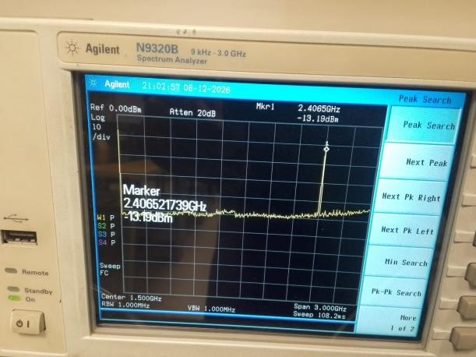
\includegraphics[width=0.7\textwidth]{image1.png}
		\caption{Oscilloscope capture of the amplitude-modulated noise waveform (sawtooth carrier).}
		\label{fig:am_noise}
	\end{figure}
	
	\begin{figure}[H]
		\centering
		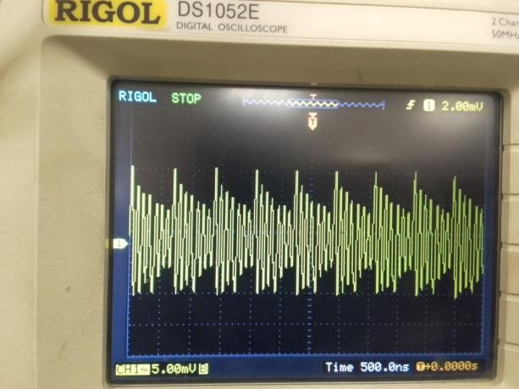
\includegraphics[width=0.7\textwidth]{image2.png}
		\caption{Oscilloscope capture confirming RF output centered near 2.4 GHz after upconversion.}
		\label{fig:rf_output}
	\end{figure}
	
	
	
	\section{Applications of the Project}
	The dual-band directional jamming system developed in this project has several potential real-world applications, spanning security, defense-support, and educational domains. Each application area is discussed below along with the specific system characteristics that make it relevant.
	\begin{table}[htbp]
		\centering
		\caption{Equipment and Components Used in the Proposed System}
		\label{tab:equipment}
		\renewcommand{\arraystretch}{1.3}
		\begin{tabularx}{\textwidth}{|l|X|}
			\hline
			\textbf{Equipment / Component} & \textbf{Purpose} \\ \hline
			
			RIGOL DS1052E Digital Oscilloscope &
			Time-domain verification of baseband, modulated, and mixer-stage waveforms. \\ \hline
			
			Agilent N9320B Spectrum Analyzer &
			Frequency-domain verification of RF output and spurious content. \\ \hline
			
			Arduino Microcontroller Platform &
			Digital pseudo-random baseband noise generation (PWM/DAC). \\ \hline
			
			AD-830+ Active Mixer &
			Frequency upconversion (baseband to RF). \\ \hline
			
			RF2126 RF Power Amplifier &
			RF signal amplification prior to radiation. \\ \hline
			
			Vector Network Analyzer (VNA) &
			Practical return-loss ($S_{11}$) and VSWR verification of the fabricated antenna. \\ \hline
			
		\end{tabularx}
	\end{table}
	
	\subsection{Physical Security and Anti-Surveillance}
	The system can be deployed to disrupt unauthorized wireless microphones, hidden cameras, or covert transmitters operating in the 2.4 GHz and 5.8 GHz ISM bands within sensitive or restricted premises. Many low-cost covert surveillance devices rely on these unlicensed bands precisely because they are inexpensive and require no specialized RF hardware to build; a directional jammer with sufficient gain and correctly matched antenna can deny such a device’s uplink within a defined sector – for instance, a single room or hallway – without requiring the defender to first locate or identify the specific device. Because the antenna is directional, security personnel can sweep the beam across a room or point it at a suspected source, limiting collateral disruption to the rest of the facility’s authorized wireless infrastructure.
	\subsection{Counter-Drone (Anti-UAV) Applications}
	Since many commercial drones rely on 2.4 GHz and 5.8 GHz links for control and video downlink, a directional jammer can be used to sever communication with an unauthorized drone in a targeted airspace sector without broadly disrupting the surrounding RF environment. This is particularly relevant near airports, correctional facilities, stadiums, and government or military installations, where uncontrolled drone incursions pose both privacy and physical-security risks. A directional system, as opposed to an omnidirectional one, allows an operator to track and jam a specific drone’s flight path while leaving nearby legitimate Wi-Fi networks, telemetry links, and other authorized
	2.4/5.8 GHz devices largely unaffected.
	\subsection{Research and Academic Use}
	The project also serves as a practical platform for studying RF signal chains, jamming techniques, spread-spectrum communication, and antenna design, and can be extended by future students to explore adaptive or spread-spectrum jamming strategies. The modular architecture developed here noise source, modulator, mixer, amplifier, and antenna, each independently testable lends itself well to being used as a teaching platform in RF and communications laboratory courses, where individual stages can be swapped, measured, and characterized in isolation. The inclusion of the 41.75 MHz PN sequence generator, though not required for the baseline noise-jamming implementation, provides a ready foundation for follow on student projects investigating DSSS based jamming or spread-spectrum communication techniques more broadly.
	\subsection{Event and Facility Spectrum Protection}
	Directional jamming can be used in controlled, authorized settings (e.g., examination halls, secure conference rooms, or sensitive negotiation venues) to prevent unauthorized wireless data exfiltration over common ISM-band links, while limiting collateral interference through the antenna’s directional radiation pattern. In examination settings, for example, a directional jammer aimed at a seating area could disrupt attempts to use WiFi- or Bluetooth-based cheating devices without affecting the invigilation staff’s own communication equipment located outside the jamming sector.
	\subsection{Electronic Warfare and Defense-Support Research}
	At a broader level, the noise-jamming and (planned) spread-spectrum jamming techniques explored in this project are foundational to the field of electronic warfare (EW) and electronic countermeasures (ECM). While the system built in this project is a lowpower, laboratory-scale prototype and is not intended for tactical deployment, the underlying principles – noise generation, spectral shaping, frequency agility, directional radiation, and power amplification – are directly analogous to those used in larger-scale, higher-power defense-oriented jamming systems, making the project a relevant stepping stone for students interested in pursuing further study or careers in RF-based defense electronics.
	\section{Project Plan}
	\subsection{Project Milestones}
	The project was split into Part I and Part II. The tasks were divided in reporting periods and were equally divided among the three group members (Rameen Khan, Mohammad Hasnain Abbasi and Mahroona Mariam Khan). Each member contributed to the noise-generation, RF and antenna-design aspects of the system under the supervision of Dr. Noor Muhammad Khan. Work was recorded in a series of biweekly progress reports, numbered serially as Report 1 to Report 14. Part I consists of Reports 1-8 and Part II consists of Reports 9-14. Each report covers a two-week period and includes a summary of objectives, accomplishments, obstacles encountered, and future actions.This ensured that the project went through a disciplined incremental hardware bring up process rather than trying to design and integrate the whole system in one pass.
	
	\vspace{0.5cm}
	
	The first part of the project (Reports 1-8) began with a research and architecture selection phase in September 2025, where the team first surveyed three candidate methods of superimposing wideband noise onto an RF carrier, namely, the baseband modulation (mixer-based), direct RF noise generation, and a digital vector-signal-generator (VSG) approach and, after comparing them on flexibility, complexity, and cost, settled on the baseband modulation (mixer-based) architecture as the most suitable for an undergraduate-scale dual-band prototype (Report 1).This was followed in October of 2025 with a deeper study of wideband noise-spreading techniques. The team reviewed barrage jamming, DSSS, and CDMA/TDMA/FDMA multiple-access schemes, implemented in theory a linear-feedbackshift-register (LFSR) based PN-sequence generator, and built an initial Zenerdiode wideband noise source that was amplitude-modulated to produce a prototype jamming waveform (Report 2). The team then built a working 320 kHz narrowband Zener-diode noise jammer and planned to expand this to a wideband, direct-sequence spread-spectrum (DSSS) signal using a PN-sequence generator and double-balanced mixer (Report 3).This was followed by the finalization of the noise-source circuit and instrumentation of the PN-sequence generator. In the process, the team ran into a major supply-chain hurdle the unavailability of standard four-quadrant analog multiplier ICs (AD835, AD834/834A, ADL5390, LT5517). Hence, the team looked into a discrete log–antilog multiplier as an alternative analog multiplication technique (Report 4). In Report 5, a component procurement phase is described, where the core hardware for the wideband prototype was ordered: a Teensy 4.1 microcontroller, an AD834 RF multiplier, an ADL5801 RF mixer, an HMC219 RF switch, and the RF2126 power amplifier.The team then went with a way to do things. They used Arduino to make baseband noise and the AD-830+ active mixer to change the frequency. This is talked about in Report 7. After the mixer they added an RF power amplifier stage. This was because the mixer did not produce an enough signal. The amplifier helped by making the signal 20 to 25 times stronger which is shown in Report 8. The team used the AD-830+ mixer and the RF power amplifier stage to make the signal stronger. The Arduino-based baseband noise generation was also a part of this process.
	
	\vspace{0.5cm}
	
	Part II of the experiment (Reports 9-14) started from a hardware-related digital-logic problem: A pseudo-noise sequence generator based on a 7-bit LFSR using Verilog HDL language was implemented in a Nexys 2 FPGA board, and its output was demonstrated through an onboard LED to practice what was learned about pseudo-noise generation and create a building block for future DSSS jamming (Report 9).A number of different jamming techniques are described at the conceptual level, with narrowband noise jamming eventually being selected as the basis for development of the working prototype. A 41.75 MHz PN sequence generator is suggested as the starting point for designing systems capable of producing jamming signals based upon direct-sequence spread spectrum (DSSS) [Report 10]. 
	
	\vspace{0.5cm}
	
	Antenna impedance-matching design and simulations are carried out leading to a simulated return loss of better than -15dB when a single-stub matching network is introduced into the circuitry [Report 11]. Practical implementation of the noise generation and amplitude modulation stages of the signal path is undertaken  utilising a sawtooth carrier [Report 12].
	
	\vspace{0.5cm}
	
	Frequency upconversion to 2.4GHz takes place alongside the integration of an appropriate power amplifier (RF2126) [Report 13]. A physical 2.4GHz directional antenna is fabricated and integrated into the completed RF transmission chain, allowing the initial testing of the entire system via an over-the-air transmission [Report 14]. Summary tables listing all the key developments made in each phase, along with an even more granular breakdown report-by-report, can be seen in Tables 1.3 \& 1.4 below:
	\begin{longtable}{|p{2cm}|p{2cm}|p{10cm}|}
		\caption{Project Milestones by Report} \label{tab:milestones} \\
		\hline
		\textbf{Part} & \textbf{Report(s)} & \textbf{Milestone} \\
		\hline
		\endfirsthead
		
		\hline
		\textbf{Part} & \textbf{Report(s)} & \textbf{Milestone} \\
		\hline
		\endhead
		
		Part I & R1 &
		Research and comparison of noise-on-carrier generation methods (baseband modulation, direct RF generation, digital VSG); selection of the baseband modulation (mixer-based) architecture. \\
		\hline
		
		Part I & R2 &
		Study of wideband noise-spreading techniques (barrage jamming, DSSS, CDMA/TDMA/FDMA); LFSR-based PN-sequence theory; construction of an initial Zener-diode wideband noise source with AM. \\
		\hline
		
		Part I & R3 &
		Narrowband (320 kHz) Zener-diode noise-jammer construction; investigation of DSSS spreading using a PN-sequence generator and double-balanced mixer to extend coverage toward the 2.4 GHz ISM band. \\
		\hline
		
		Part I & R4 &
		Finalization of the noise-source circuit and PN-sequence generator instrumentation; investigation of a discrete log--antilog analog multiplier following the unavailability of standard multiplier ICs. \\
		\hline
		
		Part I & R5 &
		Procurement of core wideband-prototype hardware: Teensy 4.1, AD834 RF multiplier, ADL5801 RF mixer, HMC219 RF switch, and RF2126 amplifier. \\
		\hline
		
		Part I & R7--R8 &
		Baseband noise generation using Arduino; RF upconversion using the AD-830+ mixer; integration of the RF power amplifier stage. \\
		\hline
		
		Part II & R9 &
		FPGA-based (Nexys 2, Verilog) hardware implementation of a 7-bit LFSR PN-sequence generator, verified via LED output. \\
		\hline
		
		Part II & R10--R11 &
		Selection of narrowband noise-jamming approach; conceptual design of the 2.4 GHz jammer architecture; antenna impedance-matching design and simulation. \\
		\hline
		
		Part II & R12--R13 &
		Noise generation and Amplitude Modulation (AM) with sawtooth carrier; frequency upconversion to 2.4 GHz; RF2126 power-amplifier integration. \\
		\hline
		
		Part II & R14 &
		Integration of the fabricated directional antenna with the RF transmission chain; initial over-the-air testing. \\
		\hline
		
	\end{longtable}
	\begin{longtable}{|p{1.5cm}|p{2cm}|p{5cm}|p{6cm}|}
		\caption{Report-wise Breakdown of Objectives and Achievements (Reports 1--14)}
		\label{tab:reports} \\
		\hline
		\textbf{Report} & \textbf{Period} & \textbf{Primary Objective} & \textbf{Key Achievement} \\
		\hline
		\endfirsthead
		
		\hline
		\textbf{Report} & \textbf{Period} & \textbf{Primary Objective} & \textbf{Key Achievement} \\
		\hline
		\endhead
		
		R1 & Sep 2025 &
		Research and compare noise-on-carrier generation methods &
		Selected baseband modulation (mixer-based) as the target architecture; defined key performance metrics (PSD flatness, bandwidth, NPR, carrier suppression). \\
		\hline
		
		R2 & Oct 2025 &
		Wideband noise spreading theory (PN codes, LFSR); build initial Zener noise source &
		Implemented LFSR PN-spreading theory; reviewed barrage/DSSS/CDMA techniques; built and AM-modulated a Zener-diode wideband noise source. \\
		\hline
		
		R3 & Sep--Dec 2025 &
		Narrowband (320 kHz) Zener-noise jammer; DSSS spreading plan &
		Built 320 kHz Zener-diode noise source; designed PN-sequence (LFSR) generator. \\
		\hline
		
		R4 & Dec 2025 &
		Finalize noise source; instrument PN generator; source analog multiplier and mixer-based spreading/upconversion plan for the 2.4 GHz band &
		Verified noise source and PN generator timing; investigated log--antilog discrete multiplier after standard multiplier ICs proved unobtainable. \\
		\hline
		
		R5 & Jan 2026 &
		Hardware research and component procurement &
		Ordered Teensy 4.1, AD834, ADL5801, HMC219, and RF2126; clarified overall wideband system architecture. \\
		\hline
		
		R7 & Jan--Feb 2026 &
		Baseband noise generation (Arduino) and RF upconversion via AD-830+ mixer &
		Verified frequency translation ($f_{RF}=f_{LO}\pm f_{IF}$) and narrowband RF output on a spectrum analyzer. \\
		\hline
		
		R8 & Feb 2026 &
		Integration of an RF amplifier stage after the mixer &
		Achieved 20--25 dB gain with stable operation; identified spurious-signal and thermal-management challenges. \\
		\hline
		
		R9 & Mar 2026 &
		FPGA (Nexys 2) implementation of a 7-bit LFSR PN-sequence generator &
		Verified pseudo-random output on Verilog hardware via LED; documented applications (CDMA, cryptography, BIST) and limitations of LFSR-based PN generation. \\
		\hline
		
		R10 & Mar--Apr 2026 &
		Selection of jamming technique; preliminary jammer architecture &
		Selected narrowband noise jamming; proposed a 41.75 MHz PN-sequence generator for future DSSS use. \\
		\hline
		
		R11 & Apr 2026 &
		Antenna impedance matching and return-loss optimization &
		Simulated $S_{11} < -15$ dB at 2.45 GHz using single-stub matching; VSWR $< 1.5$. \\
		\hline
		
		R12 & Apr--May 2026 &
		Noise generation and AM modulation with sawtooth carrier &
		Verified stable AM-modulated waveform on the oscilloscope. \\
		\hline
		
		R13 & May--Jun 2026 &
		Frequency upconversion to 2.4 GHz and RF2126 amplifier integration &
		Verified 2.4 GHz RF output on the spectrum analyzer with amplification. \\
		\hline
		
		R14 & Jun 2026 &
		Integration of fabricated directional antenna with RF chain &
		Completed hardware assembly; performed first over-the-air test of the full 2.4 GHz chain. \\
		\hline
		
	\end{longtable}
	\subsection{Targeted Sustainable Development Goals}
	Table 1.5 lists the United Nations Sustainable Development Goals (SDGs) targeted during the implementation of this project.
	\begin{table}[htbp]
		\centering
		\caption{List of Targeted Sustainable Development Goals}
		\label{tab:sdg}
		\renewcommand{\arraystretch}{1.3}
		\begin{tabularx}{\textwidth}{|p{2cm}|p{4cm}|X|}
			\hline
			\textbf{SDG No.} & \textbf{SDG} & \textbf{Relevance to the Project} \\
			\hline
			
			SDG 9 &
			Industry, Innovation and Infrastructure &
			Development of an indigenous RF hardware system contributing to local research and innovation in electronic countermeasure technology. \\
			\hline
			
			SDG 16 &
			Peace, Justice and Strong Institutions &
			Enhancing physical and information security by countering unauthorized wireless surveillance and communication devices. \\
			\hline
			
			SDG 4 &
			Quality Education &
			Provides a hands-on RF engineering learning platform for future final year project students. \\
			\hline
			
		\end{tabularx}
	\end{table}
	\subsection{Team Composition and Responsibilities}
	
	In Table 1.6 we have listed the group members and their primary areas of responsibility inside the project as described by the respective biweekly reports (balanced distribution between the various task domains / workstreams “baseband/digital”, “RF/mixer amplifier” and “antenna design”)
	
	\begin{table}[H]
		\centering
		\caption{Group Members and Primary Responsibilities}
		\label{tab:group_members}
		\renewcommand{\arraystretch}{1.3}
		
		\begin{tabularx}{\textwidth}{|p{4cm}|p{2.5cm}|X|}
			\hline
			\textbf{Student Name} & \textbf{Reg. No.} & \textbf{Primary Area of Responsibility} \\
			\hline
			
			Rameen Khan &
			BEE223009 &
			Baseband noise generation and Arduino-based digital signal generation. \\
			\hline
			
			Mohammad Hasnain Abbasi &
			BEE223017 &
			RF mixer/upconversion stage and RF power amplifier integration. \\
			\hline
			
			Mahroona Mariam Khan &
			BCPE223021 &
			Antenna design, impedance matching, and directional-radiation testing. \\
			\hline
			
		\end{tabularx}
	\end{table}
	\subsection{Project Timeline}
	In summary, the timeline for completing the project began during part I of the Final Year Project with Research and Conceptual Groundwork in September 2025 [noise-on-carrier method selection, Report 1] and continued throughout October 2025 [Wideband Noise-Spreading Theory + Initial Zener-Diode Noise Source, Report 2]. The latter half of part I (Narrowband-Jammer Construction, Component Sourcing, and Initial RF Hardware Bring-Up) was completed by February 2026 [Part I Reports 1-8], while part II included additional work on the design in March 2026 [FPGA-Based PN-Generator Work], followed by a full system redesign and hardware implementation before moving to integration testing in June 2026 [Part II Reports 9-14].
	
	\vspace{0.5cm}
	
	A detailed timeline can be found in Fig. 1.5 below as a Gantt chart outlining the approximate length of time spent on each major task over the course of the project alongside the specific biweekly periods mentioned above in Sect. 1.6.1.
	\subsection{Report Organization}
	The rest of the paper is organized as follows. Chapter 2 is the literature review which consists of the following sections. This section will introduce the background theory on radio frequency (RF) jamming, the common modulation techniques for signal transmission, the current technology/projects on electronic jamming and their capabilities, the potential research directions for electronic jamming technologies, the limitations of the current technologies and at the end of this section the formal problem statement will be presented. 
	
	Chapter 3 details the design approaches and the implementation details of the dual-band directional jamming system. 
	
	It will comprise sections on hardware design on its different modules, which includes noise generation, signal modulation, signal up conversion, power amplification and antenna array and it will also cover the methods of analysis and a working prototype description. Chapter 4 covers the methods and technologies (both hardware and software/simulation based) that were used throughout this project.
			
		\begin{figure}[H]
			\centering
			\begin{ganttchart}[
				hgrid,
				vgrid,
				x unit=0.9cm,
				y unit chart=0.7cm,
				title height=1,
				bar height=0.6,
				group height=0.7,
				milestone height=0.6,
				bar/.style={fill=cyan!40},
				title/.style={draw=none, fill=none},
				title label font=\small,
				bar label font=\small
				]{1}{10}
				
				\gantttitle{Sep}{1}
				\gantttitle{Oct}{1}
				\gantttitle{Nov}{1}
				\gantttitle{Dec}{1}
				\gantttitle{Jan}{1}
				\gantttitle{Feb}{1}
				\gantttitle{Mar}{1}
				\gantttitle{Apr}{1}
				\gantttitle{May}{1}
				\gantttitle{Jun}{1} \\
				
				\ganttbar{R1}{1}{1} \\
				\ganttbar{R2}{2}{2} \\
				\ganttbar{R3}{1}{3} \\
				\ganttbar{R4}{4}{4} \\
				\ganttbar{R5}{5}{5} \\
				\ganttbar{R7}{6}{6} \\
				\ganttbar{R8}{7}{7} \\
				\ganttbar{R9}{8}{8} \\
				\ganttbar{R10}{8}{8} \\
				\ganttbar{R11}{9}{9} \\
				\ganttbar{R12}{9}{9} \\
				\ganttbar{R13}{10}{10} \\
				\ganttbar{R14}{10}{10}
				
			\end{ganttchart}
			\caption{Project Timeline (Gantt Chart) --- Part I (Reports 1--8) and Part II (Reports 9--14)}
			\label{fig:gantt}
		\end{figure}
		
	Chapter 5 The final section of the project, the results of the tests carried out, verification of implemented design and functionalities, a comparison against the requirements specification and the limitations of the prototype produced. Lastly the conclusion sums up the achievements, and following this is the reference section and appendix.
	
	\chapter{Literature Review}
	Even before any wires had been soldered or waveforms captured on an oscilloscope, the team devoted quite a lot of time to doing nothing but reading: textbooks about microwave engineering, patents about barrage jamming waveform generators, data sheets from manufacturers of counter-drone devices, and quite a few articles about spread spectrum anti-jamming techniques, which, to be honest, deal with the opposite problem to ours.Section 2.2 explores the two sets of technologies that are most relevant to the proposed project  commercial and military-grade counter-UAS jammers, as well as software defined radio (SDR) based jamming systems. Section 2.3 provides an analysis of two concrete projects that served as sources of inspiration for our work. Section 2.4 moves backwards to show what current directions research community takes which happen to be mainly on the defensive (anti-jamming) side, contrary to offensive approach which was aimed for in this project. Section 2.5 discusses briefly what the existing research body is missing  and which is why the problem statement of this project, described in Section 2.6, fits into that gap.
	
	\section{Background Theory}
	\subsection{What Jamming Actually Is}
	Fundamentally, radio frequency (RF) jamming is a form of denial of service (DoS) attack conducted at the physical layer.
	Rather than attempting to penetrate into the protocols of the communication channel, or to spoof a packet, or to take advantage of some software flaw, 20
	the jammer just tries to win a competition for the same band of spectrum as the receiver and succeeds in winning because of higher power levels. When the jamming signal comes to the victim receiver with enough power compared to the desired signal, measured as the jamming to signal ratio J/S, then demodulator of the receiver cannot distinguish between the required waveform and jamming and the connection becomes impossible. It is not a very sophisticated way of attacking electronic devices, but the lack of sophistication is just the reason why this kind of electronic warfare looks like a suitable topic for a project of an undergraduate student.
	
	\vspace{0.5cm}
	
	Intentional jamming is well described in the literature by a relatively small number of canonical methods, and the discussion of these should be taken in order because the choice of jamming method dictated most of the hardware choices that came afterward. Spot jamming is focused exclusively at a very narrow frequency band that is known in advance to be used by the receiver to be jammed, resulting in maximal J/S ratio for this type of jamming, while completely ineffective in case when the victim hops channels or employs unexpected broadening of the bandwidth [1, 4]. On the other hand, sweep jamming does the opposite thing and tunes the full power of the jammer to a range of frequencies instead of staying in one spot; this way, at any particular moment only a fraction of the total range is jammed, while the whole band gets covered over time [4, 13]. The sacrifice paid in this type of jamming is a lower duty cycle since the receiver operating at a fixed frequency will be jammed during the fraction of sweep cycle that coincides with the jammer's frequency tuning. The technique of choice, which the present project employs, is barrage jamming  spreading the power of the jammer over a contiguous set of frequencies simultaneously and jamming every channel in the range, while decreasing the power spectral density compared to spot jamming [1, 3, 6]. It is interesting to notice how Wikipedia's article about radar jamming mentions that early barrage jammers were so successful against 1950s radar systems that the obsolescence of long-range radar technology seemed likely – an amusing reminder of the fact that "jam everything and pray" is quite an old technique indeed [5]. The final method of deception jamming departs from simple noise completely:While noise jamming raises the level of noise in the environment, deception adds a realistic-looking, albeit false, signal  a spoof packet, a fake radar response, a falsified GPS pseudo range  to be received and interpreted erroneously by the victim receiver [1, 2]. Deception attacks are much more complicated to perform since they involve an understanding of the protocol of the victim, and they have been left out very early in the development of this research.
	
	\vspace{0.5cm}
	
	In a taxonomy paper that recently came out, the application of all four jamming types, which include spot, sweep, barrage, and deception, against small UAVs was reviewed, and it was noted that the majority of jamming methods that have been considered in anti-drone literature tend to use noise-based barrage or sweep methods on the communication channels while leaving deception for the GNSS channel due to the efficacy of spoofing a false position compared to denying the channel [2]. This corresponds perfectly to the focus of this research paper since the jammer proposed herein targets 2.4 GHz and 5.8 GHz command and video channels and noise-based barrage jamming was an obvious choice
	Figure~\ref{fig:jam-taxonomy} summarizes this taxonomy graphically, showing how the noise-based techniques (spot, sweep, and barrage) relate to the deceptive/repeater family, and marking the branch -- barrage, noise-based -- that this project's own architecture occupies.
	
	\begin{figure}[h]
		\centering
		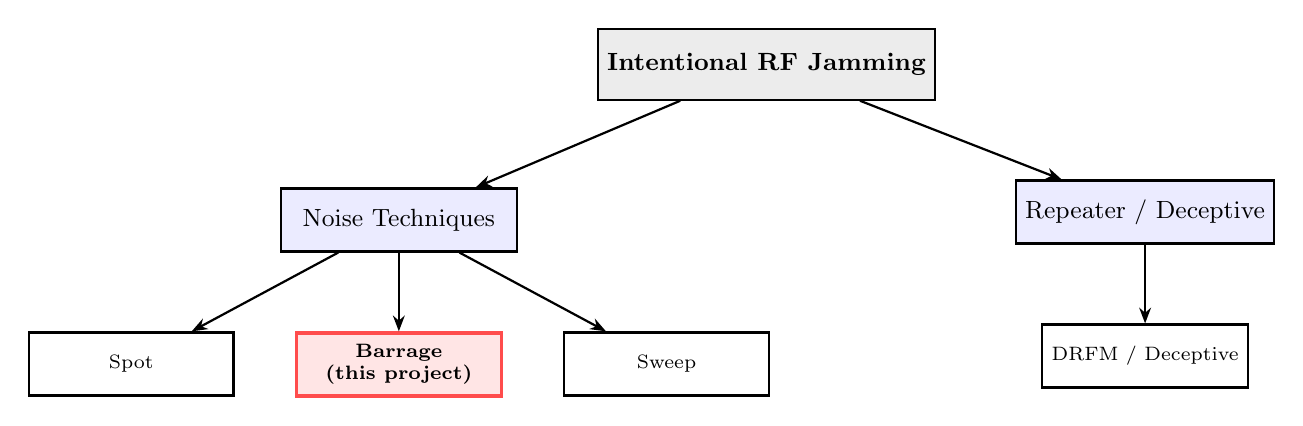
\begin{tikzpicture}[
			node distance=0.5cm and 0.5cm,
			root/.style={rectangle, draw, thick, fill=gray!15, minimum height=0.9cm, minimum width=3.2cm, align=center, font=\small\bfseries},
			branch/.style={rectangle, draw, thick, fill=blue!8, minimum height=0.8cm, minimum width=3cm, align=center, font=\small},
			leaf/.style={rectangle, draw, thick, minimum height=0.8cm, minimum width=2.6cm, align=center, font=\scriptsize},
			sel/.style={rectangle, draw=red!70, very thick, fill=red!10, minimum height=0.8cm, minimum width=2.6cm, align=center, font=\scriptsize\bfseries},
			arr/.style={-{Stealth[length=2mm]}, thick}
			]
			\node[root] (root) {Intentional RF Jamming};
			\node[branch, below left=1.1cm and 1cm of root] (noise) {Noise Techniques};
			\node[branch, below right=1cm and 1cm of root] (rep) {Repeater / Deceptive};
			\node[leaf, below=1cm of noise, xshift=-3.4cm] (spot) {Spot};
			\node[sel, below=1cm of noise] (barrage) {Barrage \\ (this project)};
			\node[leaf, below=1cm of noise, xshift=3.4cm] (sweep) {Sweep};
			\node[leaf, below=1cm of rep] (drfm) {DRFM / Deceptive};
			\draw[arr] (root) -- (noise);
			\draw[arr] (root) -- (rep);
			\draw[arr] (noise) -- (spot);
			\draw[arr] (noise) -- (barrage);
			\draw[arr] (noise) -- (sweep);
			\draw[arr] (rep) -- (drfm);
		\end{tikzpicture}
		\caption{Taxonomy of intentional RF jamming techniques, after~\cite{ref1,ref4,ref5}}
		\label{fig:jam-taxonomy}
	\end{figure}
	
	Every jamming technique reviewed above ultimately succeeds or fails according to a single figure of merit at the victim receiver: the jamming-to-signal ratio, or $J/S$, usually expressed in decibels as
	
	\[
	J/S \ (\text{dB}) = P_J + G_{J} - L_{J} - (P_S + G_S - L_S),
	\]
	where PJ and PS represent jamming and the transmitting signal’s radiated powers, respectively, GJ and GS refer to the antenna gains for both signals toward the victim receiver, and finally, LJ and LS represent the corresponding propagation losses between each of these transmitters and the victim receiver (largely dictated by the distances from each transmitter to the receiver via the free space path loss). This formula is more than just theoretical: it represents the “design formula” that this whole project was constructed on from day one, long before we ever put a name to it. The rationale behind all of the hardware choices discussed in the fourteen biweekly reports is to favor either the jammer or the transmitter through manipulating one of the four variables on the right-hand side of the above equation: selection of a power amplifier stage (Biweekly Reports 5, 8, and 13) boosts PJ, directional antenna design and impedance matching (Biweekly Report 3, and fabrication efforts in Biweekly Report 14) increases GJ toward the specific target while not wasting power elsewhere, and finally, placing the jammer closer to the intended target location reduces LJ relative to a victim receiver located farther from its legitimate transmitter.
	
	\vspace{0.5cm}
	
	where $P_J$ and $P_S$ are the radiated powers of the jammer and of the legitimate transmitter, respectively, $G_J$ and $G_S$ their antenna gains towards the victim receiver and $L_J$, $L_S$ the propagation losses (which, to a large degree, are determined by the distance between the transmitters and the receiver, along with the free space path loss, as defined by the Friis equation). Throughout the series of fourteen biweekly reports, one may see the attempt to improve one of those four factors on the right-hand side: is not just some theoretical insight -- it is, quite literally, the design equation that this whole project is based upon, even though we didn't have such a thing in mind back then. Each hardware choice recorded in the Reports~5, 8 and~13 increases the factor $P_J$; designing and matching impedance of the directional antenna in Report~3 and its manufacturing in Report~14 increase the factor $G_J$ only towards the victim receiver, but \emph{not} towards any other directions; and less explicitly, keeping the jammer physically close to the target area decreases the factor $L_J$ compared to a victim receiver which operates at a greater distance from its own legitimate transmitter.
	
	\vspace{0.5cm}
	
	where $P_J$ and $P_S$ are the radiated powers of the jammer and of the legitimate transmitter, respectively, $G_J$ and $G_S$ their antenna gains towards the victim receiver and $L_J$, $L_S$ the propagation losses (which, to a large degree, are determined by the distance between the transmitters and the receiver, along with the free space path loss, as defined by the Friis equation). Throughout the series of fourteen biweekly reports, one may see the attempt to improve one of those four factors on the right-hand side: is not just some theoretical insight -- it is, quite literally, the design equation that this whole project is based upon, even though we didn't have such a thing in mind back then. Each hardware choice recorded in the Reports~5, 8 and~13 increases the factor $P_J$; designing and matching impedance of the directional antenna in Report~3 and its manufacturing in Report~14 increase the factor $G_J$ only towards the victim receiver, but \emph{not} towards any other directions; and less explicitly, keeping the jammer physically close to the target area decreases the factor $L_J$ compared to a victim receiver which operates at a greater distance from its own legitimate transmitter.
	
	\vspace{0.5cm}
	
	The $J/S$ ratio also accounts for the recurring observation made while studying the commercially available anti-drone technology literature (Section~\ref{sec:related-tech}): vendors are always inclined towards using directional antennas with gain rather than boosting the transmitter's power directly because gain is beneficial to $G_J$ without an increase in DC power consumption, while every decibel worth of $P_J$ increase entails an increment of the amplifier's size, heat dissipation, and cost. It was exactly the choice this project made too: the RF2126 amplifier stage was chosen with an expected gain of about 20-25~dB (Report~8), but much more engineering effort was put into the antenna design and matching (Report~3) in order to make sure the gain was not lost in directions where there was no target.
	
	\vspace{0.5cm}
	
	In addition to an energy-based threshold, most real-world receivers will also suffer from what is sometimes known as \emph{desensitization} or \emph{front-end blocking}: even before the desired signal becomes completely dominated by the jamming noise in any strict $J/S$ sense, if the interfering signal is strong enough that it enters the receiver's passband, the noise figure of the receiver's low-noise amplifier or mixer will become degraded due to its going into compression, thus decreasing the sensitivity of the receiver below that predicted by $J/S$ considerations. This is part of the reason barrage and noise jammers can be effective despite being below the expected threshold based on a simple $J/S$ analysis which uses the sensitivity threshold of the receiver. The researchers of this project do not have access to calibration equipment to directly measure desensitization of the receiver, but this effect is mentioned as an example of possible cause behind the difference observed during the initial phase of over-the-air testing (Report~14) between the successful transmission of the RF signal at 2.4 GHz and its effect on the target consumer devices.
	\subsection{Noise as an Interferer}
	It’s worth briefly thinking about why noise jamming is effective; after all, this is the premise on which the entire signal chain in Chapter 3 relies. In order to demodulate the data, the receiving circuitry of the device has to compare the incoming radio signal against some assumed pattern-be that the expected constellation of QAM data, a known preamble used for symbol synchronization, or a spread code like the one described in Chapter 2. Noise has, almost by definition, none of this predictable pattern-its spectrum is flat (ideally), and its instant amplitude is unpredictable. 
	
	Once this noise signal is introduced into the receiver’s input, it lifts the minimum discernible noise floor that the automatic gain control and demodulator must operate against. 
	
	Once the noise level approaches and rises above that of the signal the receiver is trying to receive, the bit error rate increases rapidly; past a given J/S (jammer to signal ratio) ratio, the link fails irrespective of how robust the error correction scheme may be. What makes noise jamming particularly appealing is its protocol agnosticism-regardless of whether the target is using WiFi, a custom 2.4 GHz link for drone control, or a Bluetooth stream for telemetry data, to the jammer, all it needs to do is make the receiver ‘pull’ a desired signal out of a gradually rising sea of noise. For a project, we will likely be unable to reverse engineer the intricacies of each protocol, hence noise is the simplest effective solution.
	
	\subsection{Amplitude Modulation and the Role of the Sawtooth Carrier}
	Raw baseband noise itself is not yet usable as an RF interferer; it has to be placed on some carrier that gets it into the proper portion of the spectrum so that it may be radiated by reasonably sized antenna. The simplest method of achieving this is amplitude modulation (AM) where the noise signal causes the amplitude of the carrier wave to vary in accordance with the noise: The result is an output whose envelope varies like the noise. In the conventional communications domain, AM is an old fashioned technique, somewhat, because it is rather inefficient and distortable, but in a jammer, these weaknesses matter little; after all, there's no intention of cleanly demodulating the transmitted jamming signal at the other end, just sending some power out across the desired bandwidth. 
	
	\vspace{0.5cm}
	
	More importantly, however, AM is simple, involving few discrete analog components or integrated circuits, doesn't require a synchronous local oscillator at the transmitter, and if the carrier itself has a sawtooth shape rather than a pure sinusoidal shape, then this approach adds yet another layer of spectral content at harmonics of the sawtooth carrier a small bonus. 
	
	\vspace{0.5cm}
	
	This is how we arrived at the idea to use a sawtooth carrier as the baseline modulation for our device, detailed in Report's 4, 7 and 12.
	\subsection{Frequency Conversion: Mixers, Local Oscillators, and the Mixing Equation}
	
	The noise-modulated baseband or low-IF signal is still need to mix up to the target ISM band for it to interfere effectively with a 2.4GHz or 5.8GHz receiver. This is the duty of the mixer stage. A mixer is, fundamentally, an analog multiplier, it multiplies its two input signals, here it is a noise-modulated IF signal, and the LO tone, to produce sum and difference frequencies of the original signals, according to
	\[
	f_{RF} = f_{LO} \pm f_{IF}.
	\]
	
	Both the AD-830+ active mixer in Reports 7 \& 13, and the ADL5801 mixer bought in Report 5, are capable of this function (though different mixers; the former is an OP-AMP-derived video-difference amplifier often employed as a moderate frequency active mixer; the latter is a specific purpose built, high-linearity, double balanced RF mixer designed for cellular and ISM front ends). Either way, function requires driving the LO port hard enough - typically +7 dBm, or thereabouts, for mixers of this type - as the output LO drive is insufficient causes conversion gain loss and significant spur product increase, which the team experienced directly in Report 7 and described in its challenges. Mixer also produce undesirable other mixing product outputs inevitably, including the LO drive feeding directly to the output and higher intermodulation products as the result of its inherent nonlinearity, which are seen on the spectrum analyser during reports 7, 8, \& 13 and the attempt to minimise LO drive, impedance matching and eventually bandpass filters appear on the challenge sections in each of the Reports.
	
	\subsection{RF Power Amplification}
	
	The output from a passive or mildly active mixer stage will usually be far too low to provide a useful jamming impact once radiated, therefore it is necessary to use a RF power amplifier stage in order to boost the signal to a level capable of being useful at the antenna. This project used amplifier stages at various points in its lifecycle; first a broadband amplifier providing approx 20--25~dB gain (Report 8), and then the RF2126 power amplifier which has been integrated as part of the 2.4~GHz mixer chain (Reports 5 and 13). One of the main trade-offs with any amplifier stage in a jamming system is the compromise between gain and linearity: a high gain is desirable in order to reach a substantial radiated power level, but if the amplifier is run into compression or saturation then the normally-noise-like spectral shape of the signal will be severely altered, with the generation of harmonic content. 
	
		
	Related is the question of heat management: running a power amplifier consistently near its stated limit can inevitably result in significant amounts of heat that, unless effectively removed, can lead to instability in gain over time -- something that Report 8's 'problems' section raised.
	
	\subsection{Spread-Spectrum Techniques and Pseudo-Noise Sequences}
	
	Although the working prototype ultimately implemented narrowband noise jamming rather than a fully spread-spectrum signal, a substantial portion of the early project (Reports~1 through~4, and again in Report~9) was devoted to studying direct-sequence spread spectrum (DSSS) as a way of intentionally broadening a narrowband interferer into something closer to a wideband, noise-like signal covering a much larger fraction of the target ISM band. The mechanism is worth explaining because it recurs throughout the report. In DSSS, a data (or, in the jamming case, a noise) signal is multiplied by a much higher-rate pseudo-random binary sequence -- the PN code -- before transmission. Because the PN code's chip rate is many times higher than the underlying signal's own bandwidth, the multiplication spreads the transmitted energy over a correspondingly wider bandwidth~\cite{ref7,ref8,ref9}. In a conventional communications context this spreading is what gives DSSS its resistance to narrowband interference and jamming -- a point re-iterated across nearly every DSSS reference consulted for this survey~\cite{ref7,ref8,ref9,ref10} -- since a narrowband jammer only damages a small slice of the receiver's despread signal, while the receiver's correlator recovers the rest. For a jammer, though, the same spreading mechanism can be turned around and used offensively: instead of despreading a wanted narrowband signal at the receiver, the transmitter uses a PN code to deliberately spread a noise-like interference signal across the same wide band that a target DSSS system (such as WiFi's 802.11b physical layer, historically) occupies, denying the target's despreading gain advantage.
	Figure~\ref{fig:dsss-spread} sketches the basic spectral effect of this process: a narrowband signal, once multiplied by a much-higher-rate PN chip sequence, has its energy spread across a bandwidth roughly equal to the chip rate, lowering its power spectral density even though the total signal power is unchanged.
	
	\begin{figure}[h]
	\centering
	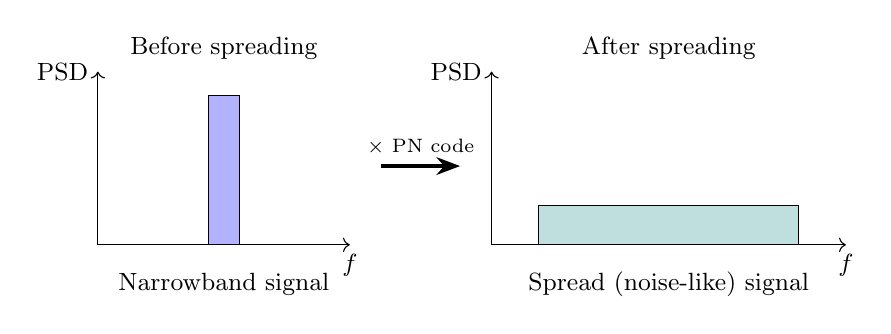
\begin{tikzpicture}[font=\small]
		% Narrowband spectrum (left)
		\draw[->] (0,0) -- (3.2,0) node[below]{$f$};
		\draw[->] (0,0) -- (0,2.2) node[left]{PSD};
		\draw[fill=blue!30] (1.4,0) rectangle (1.8,1.9);
		\node at (1.6,-0.5) {\small Narrowband signal};
		\node at (1.6,2.5) {\small Before spreading};
		
		% Arrow
		\draw[-{Stealth[length=3mm]}, very thick] (3.6,1) -- (4.6,1) node[midway, above, font=\scriptsize]{$\times$ PN code};
		
		% Wideband spectrum (right)
		\draw[->] (5,0) -- (9.5,0) node[below]{$f$};
		\draw[->] (5,0) -- (5,2.2) node[left]{PSD};
		\draw[fill=teal!25] (5.6,0) rectangle (8.9,0.5);
		\node at (7.25,-0.5) {\small Spread (noise-like) signal};
		\node at (7.25,2.5) {\small After spreading};
	\end{tikzpicture}
	\caption{Conceptual effect of DSSS spreading on signal bandwidth and power spectral density, after~\cite{ref7,ref8,ref9}}
	\label{fig:dsss-spread}
	\end{figure}
	PN codes like these are almost always generated with linear feedback shift registers (LFSRs), a string of flip-flops with taps that are combined by XOR gates based on a primitive polynomial so that the register cycles through the maximum possible $2^n-1$ states for an n-bit register before repeating\cite{ref7}. An LFSR generated PN code has favorable autocorrelation properties-that is, to a correlator not synced to it, the sequence appears to be mostly white noise-but is still fully reproducible, which enables a cooperating receiver to duplicate the sequence to descramble the signal\cite{ref7,ref8}. This was precisely the arc our own PN sequence work took as well: Report~2 examined LFSR theory and explored PN spreading in context of CDMA, TDMA, and FDMA multiple access, report~3 produced an LFSR-based PN generator with double-balanced mixer designed to spread 320 kHz of narrowband noise toward 2.4 GHz, and report~9, slightly out of order among other work involving RF hardware but interesting from a digital logic perspective on its own, implemented a 7-bit LFSR PN sequence generator in Verilog on a Nexys~2 FPGA and verified its pseudorandomness using an onboard LED. 
	
	The value called the processing gain of a DSSS system-typically in the range 10–60 dB for common designs\cite{ref10)- quantifies how much spreading value a system provides, defined as the spread band width divided by the original signal bandwidth in dB.} 
	
	Though report~10's proposed 41.75 MHz PN generator did not end up making it into the final working 2.4 GHz prototype of this project on schedule, it has been documented as a discrete extension path that can be explored in future work.
	\subsection{Antenna Fundamentals, Directionality, and Impedance Matching}
	The final stage in the signal chain, the antenna, performs two simultaneous tasks: transforming the guided signal on the transmission line into an outgoing, radiating electromagnetic wave and defining where that radiation is sent. This second task is what differentiates the directional jammer from the omnidirectional jammer and was explicitly part of its early design specifications. A truly omnidirectional antenna radiates energy equally in all azimuth directions, which is convenient when the target's direction is uncertain but results in inefficient and potentially disruptive use of spectrum when the target is located in a general direction. 
	
	A directional antenna, on the other hand, beams the same total power in a smaller segment of angles at the expense of reduced or null transmission in directions outside the sector. 
	
	When the same amount of transmit power is radiated by an omnidirectional versus a directional antenna, the latter is inherently more powerful in the intended direction -- a tradeoff the jammer will always accept. Commercial jammer literature even states that a relatively weak (5 W) directional 2.4 GHzjammer can effectively shut down many commercial drone models at range (approaching half a km, whereas an omnidirectional would require perhaps three or four times this power) \cite{ref11}.
	
	However, for maximum transfer of power from amplifier to antenna, the input impedance of the antenna must be matched to the impedance of the feedline and the output of the amplifier. Here, that value was 50~$\Omega$ for every device in the RF chain. If the antenna input impedance is not 50~$\Omega$, some fraction of the power incident on it will be reflected, rather than radiated. 
	
	This can be measured by VSWR or return loss $S_{11}$ in dB~\cite{ref16,ref17}. 
	
	VSWROf 1:1(or $S{11} \rightarrow -\infty$~dB) represents an ideal match. Values below 2:1(or about -10~dB for $S{11}$) are generally considered acceptable for most RF applications, while values less than 1.5:1(around -13.5~dB for $S{11}$) are considered excellent~\cite{ref17}. This project targeted $S{11} < -15$~dB or VSWR < 1.5 at 2.45~GHz, which was achieved using a simple single stub match described later in this article.
	
	\vspace{0.5cm}
	
	Single-stub matching is a time-honored technique in microwave engineering used to eliminate a mismatched impedance at one particular design frequency: An open- or short-circuited transmission-line stub of precisely the right length is connected in shunt to the main feed line at exactly the right distance from the load so that the reactive part of the stub compensates for the imaginary part of the mismatched load impedance and moves the real part of the impedance onto the characteristic-admittance circle of the matched line \cite{ref16}. The technique is relatively easy to build on a PCB, as it needs no inductors or capacitors but merely some extra transmission line; however, as a single-frequency solution it naturally has less bandwidth than a broadband matching circuit, and it will need to be retuned if the design frequency shifts significantly - this is considered an acceptable price to pay since matching at only the target 2.45 GHz frequency (at the center of the target ISM band) is sufficient. In our simulation the addition of this network improved the return loss, the result shown in Report~3 was, from an initially unacceptable value of around -6dB (the fabricated patch impedance measured about 70 Ohm in the 50 Ohm line), to over -15 dB with the subsequent mismatch loss down from ~0.8 dB to under 0.1 dB.
	
	\subsection{Measurement and Verification Methodology}
	
	One issue that keeps coming up again and again in RF literature but it's hard to truly realize the importance of it until it actually comes time to put it in the lab is that the characteristics of a jamming signal: center frequency, occupied bandwidth, output power, and spectral purity don't mean anything unless they've actually been \emph{measured} -- not just simulated or guessed from values in data sheets. At every step along the signal chain this project depended on the combination of two instruments, one for the time-domain-view of the waveforms (at all stages from baseband, to modulated to the mixer output) the other for the frequency-domain-view of the RF output, including out-of-band spectral impurities -- a digital storage scope and a spectrum analyzer respectively. The scope is the natural instrument for checking that a waveform has the correct \emph{shape} -- i.e., that the sawtooth carrier doesn't have some extra spurious content on top of it, that the envelope of an AM signal properly follows the waveform being AM'ed, or that a mixer's IF drive and LO drive levels are appropriately within bounds. 
	
	The spectrum analyzer is the natural instrument for checking that a signal falls in the desired \emph{frequency} range -- but it's just as important as the scope in revealing a signal defect that has been totally invisible on a time-domain display -- for instance, a certain level of LO bleed-through, a mirror image frequency (or image signal), out-of-band harmonics, etc. 
	
	At almost every point the results of these two instruments, used together, were of key importance, such as the case in Report~8 where we had a perfectly functioning mixer as evidenced by its time-domain output, but the spectrum analyzer showed the existence of unwanted spurious output needing more filtering.
	
	Secondly, a further similar point of methodology of concern in this document again, but particularly related to antenna matching (in report 3). The reported S11 and VSWR for the single stub matching was from circuit simulations. These were not achieved from direct VNA measurement because of lack of access to the equipment during that reporting period -- a stated challenge listed within that report, and a fair constraint for me to be transparent about; as while matched performance is an essential stage in design. This will not include fabricating tolerances, losses at connectors, enclosure size effects on the actual radiation conditions etc, that will move the actual measured S11 values away from those achieved by simulation -- should this report make reference to own values of S11 and VSWR it is well to remember these are intended design values, not those that would be measured on a bench, once a VNA can be used to take a measurement of it -- again referenced more directly in the limitation of chapter 5.
	
	\subsection{Summary of the Theoretical Foundation}
	
	Viewed together, the theory reviewed in this section bears an almost one-to-one relationship to the block diagram of the system introduced in Chapter 1 (Figure 1.2): the interfering waveform is constructed by noise generation and AM modulation; the mixer and local oscillator translate this to the band of interest; the power RF power amplifier provides the power to usable level, with close attention to linearity and heat; and finally the directional, impedance matched antenna provides efficient radiation of the power in the correct direction. The next several chapters take a look around, at the many ways other people -- commercial, military and academia -- have attacked roughly the same problem.
	\section{Related Technologies}
	\label{sec:related-tech}
	The closest related technology areas are these two categories: the world of commercial and defense counter-UAS (counter-unmanned-aerial-system) jammers (hardware whose function is to do the same thing this prototype project is trying to do at much bigger scale/budget) and the world of SDR (software-defined-radio) jamming systems (used primarily by security researchers and academia, and that attack the problem of generating radio waves from the software side). It was useful to look at these two technologies as they represent opposing implementation philosophies (hard analog/RF hardware vs flexible general-purpose radio software), and my own hardware implementation architecture wound up taking some design influences from both worlds.
	
	\subsection{Related Technology 1: Commercial and Military Counter-UAS Jamming Systems}
	The commercial anti-drone jamming market is frankly, huge and looking at a sample of publicly traded products immediately reveals that the 2.4~GHz and 5.8~GHz ISM bands targeted by this project is indeed where the industry focus is concentrated. This is not coincidental, as approximately 90~\% of commercial drone command and control links use these two bands, despite a considerably larger pool of frequencies allocated by the International Telecommunications Union for UAV command and control~\cite{ref13}. Systems surveyed in this paper varied from a handheld, rifle shaped “jammer gun” with a single digit watt of power and a built in directional antenna to backpack carried multi-band units that can deny GPS, 2.4 GHz and 5.8 GHz bands from a single case and up to base stations and vehicle mounted units that broadcast many watts of power across multiple simultaneously jammed bands~\cite{ref11,ref12,ref13}. As a typical mid-range example, one system includes ~15~dBi of directional antenna gain along with 300 W of power for roughly three times the range of an omnidirectional antenna at the same power levels, providing another real-world, concrete example of the principle of power-concentration that motivated this projects choice of directional antenna as outlined in Section~\ref{sec:background}.
	
	Operationally, these systems work in precisely the manner outlined previously: the jamming signal is set powerful enough that relative to the drone’s own command control transmitter, it can overwhelm the drone’s own receiver and it can no longer process the commands uplink, or the GNSS signals on downlink; at that point the fail-safe mechanism inherent in most consumer drones activates, telling the drone to land/hover/return to home (ref 13). Higher end systems in the military space do something even better and have built in detection on top of their jamming capability-examples are commercially marketed as CADENCE or Music ON, which will constantly monitor for the 2.4/5.2/5.8 GHz bands for presence of a drone, model, and approximate direction and only after detection and identification then enable their jam mode, at which point they can use directional beamforming rather than broadcast omni-directionally (ref 12). This is a natural extension of the approach implemented in this project (which continuously jams without any detection frontend), which we discuss as part of future work in Chapter 6. 
	
	It is also important to highlight what is not, generally, provided in the commercially marketed products listed here. 
	
	While not detailed to the level of internal circuit architectures (due to obvious commercial and export control issues), product documentation does not contain a discussion of how exactly a noise source, modulation, and mixing scheme could be laid out on circuitry, for the reason we have mentioned earlier. The contribution of this project, to some degree, lays a step below these, not in terms of sheer power or effective range, but at a circuit-level specification and explanation of a viable system that does the job for less money using standard, readily available components, exactly the level of detail that these commercial systems generally omit. Below is Table 1, which compares what I’ve deemed to be representative specifications obtained from the product brochures listed here along with those of this project’s working prototype for scaling reference purposes. As expected the range and raw power levels of commercial systems is many orders of magnitude greater; but it must be kept in mind that the commercial systems are the product of literally years of development effort with significantly larger development budgets, not on a per-hour cost compared to a 2-semester university project.
	
	\begin{table}[h]
	\centering
	\caption{Representative Commercial Counter-UAS Jammers vs.\ This Project's Prototype}
	\label{tab:commercial-comp}
	\begin{tabular}{@{}p{3.4cm}p{2.6cm}p{2.6cm}p{2.6cm}@{}}
		\toprule
		\textbf{System} & \textbf{Bands} & \textbf{Power} & \textbf{Antenna} \\
		\midrule
		Handheld jammer gun~\cite{ref29} & 2.4/5.8~GHz, GPS & 30--40~W/band & Directional, integrated \\
		Backpack multi-band unit~\cite{ref31} & 433~MHz--5.8~GHz & Up to 400~W total & High-gain directional + omni \\
		Mid-tier directional unit~\cite{ref11} & 2.4~GHz & 5~W & 15~dBi directional \\
		Detect-then-jam system (CADENCE/Music~ON)~\cite{ref12} & 2.4/5.2/5.8~GHz & Not disclosed & Omnidirectional array \\
		\textbf{This project (prototype)} & 2.4~GHz (5.8~GHz planned) & $\sim$20--25~dB amplifier gain over mixer output & Single-stub-matched directional patch \\
		\bottomrule
	\end{tabular}
	\end{table}
	
	\subsection{Related Technology 2: Software-Defined-Radio (SDR) Jamming Platforms}
	
	
	\chapter{PROJECT DESIGN AND IMPLEMENTATION}
	
	\section{Proposed Design Methodology}
	
	\subsection{Introduction}
	The rapid growth of wireless communication technologies has greatly increased the use of the unlicensed Industrial, Scientific and Medical (ISM) frequency bands. The most widely adopted of these are the 2.4 GHz and 5.8 GHz ISM bands due to their compatibility with a wide range of commercial wireless communication standards such as IEEE 802.11 Wi-Fi, Bluetooth, ZigBee, wireless surveillance systems, Internet of Things (IoT) devices, industrial telemetry systems, wireless sensors and many consumer electronic products. Due to the widespread use of these technologies, these frequency bands provide an ideal platform for studying radio-frequency (RF) signal generation, propagation, interference mechanisms and directional transmission in a controlled laboratory environment.
	\vspace{0.5cm}
	
	The aim of the project is to design and develop a dual-band directional RF interference generator, which is able to generate interference based on broadband noise at 2.4 GHz and 5.8 GHz ISM frequency bands. Unlike the software-defined radio (SDR) implementations that use digital signal processing (DSP), high-speed analog-to-digital converters (ADC), field-programmable gate arrays (FPGA) and embedded software, the proposed system is based on an analogue RF architecture. This approach facilitates troubleshooting, reduces hardware complexity and implementation cost, and provides a clear understanding of practical microwave engineering concepts.
	\vspace{0.5cm}
	The interference source in the proposed design is the avalanche noise that is naturally generated.  A Zener diode, rated at 6.8 V, in the avalanche breakdown regime produces broadband random electrical noise. The noise is filtered by a coupling capacitor and fed as modulating signal to an amplitude modulation (AM) stage with a carrier of 1 kHz. The output intermediate frequency (IF) signal is up converted to the desired microwave frequency using an ADE-30 double-balanced mixer driven by an MS-3000 Voltage Controlled Oscillator (VCO) used as the Local Oscillator (LO). The converted RF signal is then amplified by an RF2126 linear power amplifier and radiated by a high gain directional antenna.
	\vspace{0.5cm}
	
	The overall design philosophy is based on a modular RF transmit chain architecture. Each functional block performs a particular signal-processing operation, while maintaining impedance compatibility and preserving the spectral characteristics of the noise generated. This modularity implies that each subsystem can be tested, verified, optimised and replaced independently from the other stages. This also allows easy performance evaluation with laboratory equipment including oscilloscopes, spectrum analysers, vector network analysers (VNAs), RF power meters, and digital multimeters.
	\vspace{0.5cm}
	
	Compared to deterministic pseudo-random digital generators, the avalanche noise is due to microscopic collisions of carriers in the semiconductor junction. The randomness of this physical phenomenon generates broadband electrical fluctuations which are very suitable for wideband interference applications. The generated noise is continuous and non-periodic and therefore has spectral characteristics very close to those of white Gaussian noise over the frequency band of interest. This makes it an excellent broadband interference source. 
	To summarise, the proposed method is simple, reliable, cheap to implement, and educationally valuable, while demonstrating fundamental RF engineering concepts like noise generation, analogue modulation, microwave frequency conversion, impedance matching, power amplification, antenna radiation, and link-budget analysis.
	
	\subsection{Engineering Objectives}
	Before the hardware design was started, several engineering goals were established to ensure that the built prototype meets the required technical, educational and operational requirements.
	\vspace{0.5cm}
	
	First and foremost, we aimed to create a working hardware platform for injecting RF noise into the 2.4GHz and 5.8GHz ISM frequency bands by utilizing cost-effective and commercially available off-the-shelf RF components. Utilizing commercially available parts decreases hardware fabrication effort and allows for ease of sourcing and repair of the system.
	
	\vspace{0.5cm}
	
	Second, we desired to use real-world physical avalanche noise generation instead of using digitally synthesized pseudorandom sequences. Avalanche noise inherently produces broadband fluctuations that are naturally random without the use of computationally expensive digital circuits operating at high speed.
	\vspace{0.5cm}
	
	
	Third, we aimed to build the entire transmitter system around a purely linear analog RF architecture. An analog RF design preserves the continuous nature of a transmitted signal, which also means we will be able to see each processing stage of the signal in a linear fashion, facilitating troubleshooting.
	\vspace{0.5cm}
	
	
	Fourth, we aimed to match all impedances at the RF interfaces to 50 . When proper impedance matching is employed, reflection of power is minimized and the full power available from a source is transferred to the next stage or antenna. The components used in our design such as the ADE-30 mixer, RF2126 amplifier, coaxial cable,SMA connector,and the antenna, all are designed for 50 applications.
	\vspace{0.5cm}
	
	
	Fifth, we aimed to transmit the interference signal in a directional manner with a high-gain directional antenna, rather than in an omnidirectional fashion. Directional transmission concentrates the power in a certain beam, which results in an increase of the effective isotropic radiated power (EIRP) in the direction of interest.
	Finally, we sought to design this platform as an educational tool and to showcase some microwave engineering fundamentals such as:
	\vspace{0.5cm}
	\begin{itemize}
		\item[\textbullet] Avalanche noise generation
		\item[\textbullet] Analog amplitude modulation
		\item[\textbullet] Double-balanced frequency mixing
		\item[\textbullet] Voltage-controlled oscillation
		\item[\textbullet] RF power amplification
		\item[\textbullet] Impedance matching
		\item[\textbullet] Antenna theory
		\item[\textbullet] Electromagnetic wave propagation
		\item[\textbullet] Link budget analysis
		\item[\textbullet] Free-space propagation
		\item[\textbullet] RF measurement techniques
	\end{itemize}
	\vspace{0.5cm}
	Collectively, these objectives provide a comprehensive framework for understanding the design and implementation of analog RF transmission systems.
	\subsection{Design Philosophy}
	In this case, the dual-band directional interference generator was planned following the same structure as an ideal RF transmitter used by many microwave communications: Instead of creating directly RF power at the required microwave frequencies, the signal generation is realized through an ordered cascade of signal processes, each one carrying out one electrical functionality.
	\vspace{0.5cm}
			
		The Design Concept is grounded on the following principles:
		
		\begin{enumerate}
			\item \textbf{Broadband Random Noise is Generated.} The interference source is derived from Avalanche Breakdown across a 6.8 V reverse biased Zener diode. This provides a native broadband random noise source and obviates the need for digital signal generation.
			
			\item \textbf{Signal Conditioning.} A coupling capacitor will isolate the DC offset but preserve the broadband AC noise spectrum.
			
			\item \textbf{Low Frequency Modulation.} The broadband AC noise source will Amplitude Modulate a clean, stable 1 kHz sinusoidal signal and thus impart the random noise characteristics to the AM envelope.
			
			\item \textbf{Frequency Translation.} The low frequency AM signal is upconverted to the microwave frequencies by means of an ADE-30 double balanced mixer and a MS-3000 VCO. The ADE-30 outputs the sum and difference frequencies given by:
			\begingroup
			\setlength{\mathindent}{0pt}
			\begin{equation*}
				\hfill
				f_{RF}=f_{LO}\pm f_{IF}
				\hfill
			\end{equation*}
			\endgroup
				where:
			\begin{align*}
				f_{RF} &= \text{Radio Frequency output} \\
				f_{LO} &= \text{Local Oscillator frequency} \\
				f_{IF} &= \text{Intermediate Frequency (AM signal)}
			\end{align*}
					
			Since the intermediate frequency is only 1 kHz, the RF output is effectively centered at the selected LO frequency of 2.45 GHz or 5.80 GHz. The ADE-30 mixer requires approximately +7 dBm LO drive and exhibits a typical conversion loss of 4.5--6 dB, characteristics that influence the subsequent amplifier design. Given an intermediate frequency of just 1 kHz, the RF is in reality just 2.45 GHz or 5.80 GHz centered at the desired LO. This mixer (the ADE-30) requires about +7 dBm of LO drive and the typical conversion loss is in the range of 4.5 to 6 dB which helps drive the design of the subsequent amplifier.
			
			\item \textbf{Power Amplification.} The transmitted RF will require amplification after being mixed, because passive mixers have some conversion loss. This function is achieved using the RF2126 linear power amplifier.
			
			\item \textbf{Directional Radiation.} At this point, the amplified RF is fed to a directional antenna tuned to the desired frequency.
		\end{enumerate}
		
	
	\subsection{Overall System Architecture}
	The proposed dual-band directional interference generator utilizes a linear analog RF transmitter architecture which reflects the standard signal flow in typical microwave communication system architecture where every subsystem does some particular electrical task, then passes its processed signal down to the next block, until reaching the final output signal. This is in contrast with the common approaches which use very fast digital signal processors, FPGAs or software-defined radios in digital communications. Instead, this design takes advantage of the discrete analog RF devices in terms of their high reliability, less implementation cost, and convenient experimental verification. 
	\vspace{0.5cm}
	
	The whole transmitter consists of seven main blocks ( subsystems ), where these were chosen based on the suitable electrical characteristics, frequency response, input and output impedance, required power handling, and easiness of integration. 
	\vspace{0.5cm}
	
	Each block was designed separately and simulated individually before integration of the complete system. The overall block diagram of the RF transmission chain is shown below:
	\begin{figure}[htbp]
			\centering
			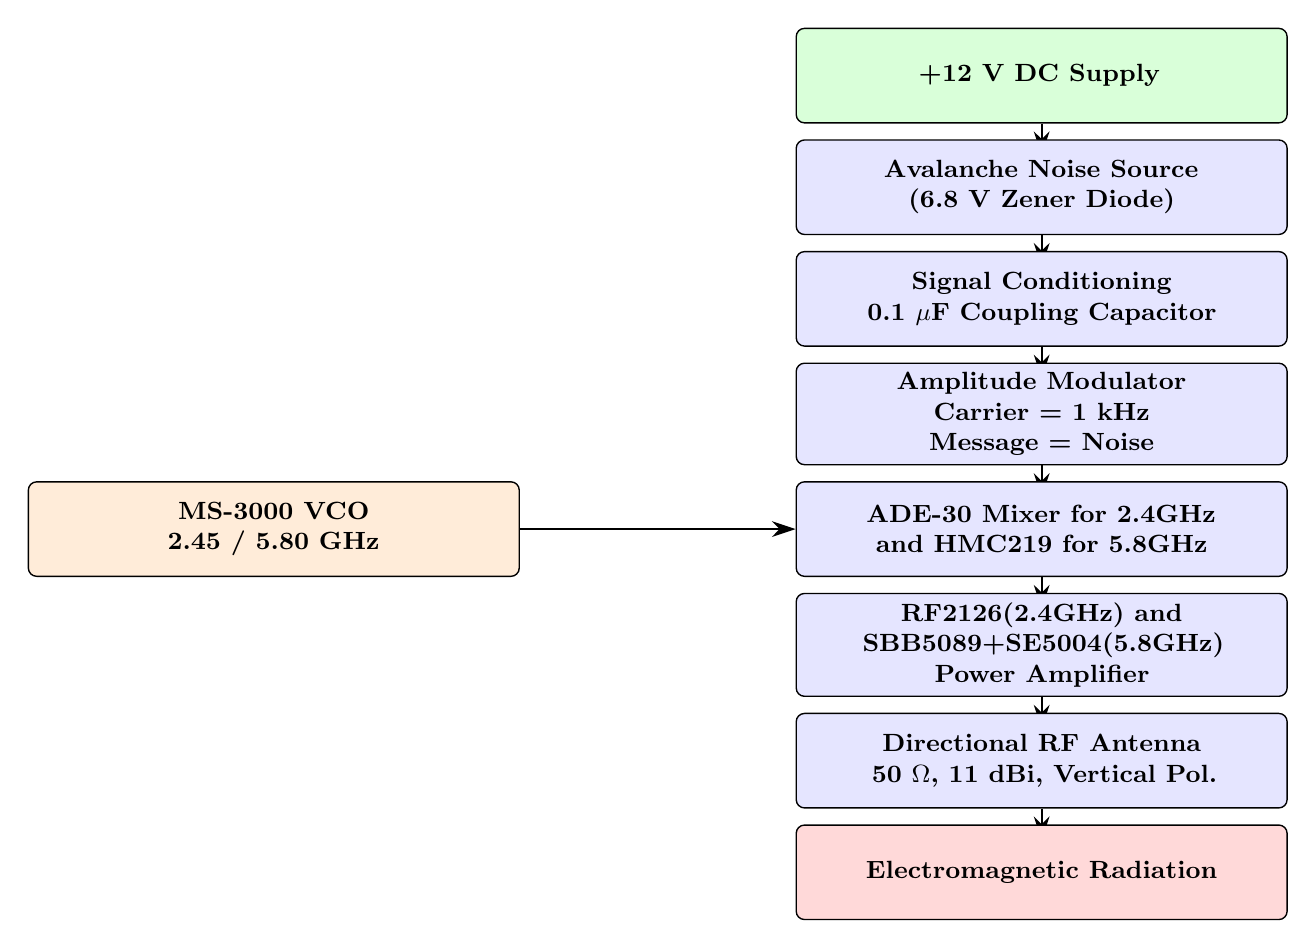
\begin{tikzpicture}[
				node distance=0.5cm,
				block/.style={
					rectangle,
					draw,
					fill=blue!10,
					text width=6cm,
					text centered,
					minimum height=1.2cm,
					rounded corners=3pt,
					font=\small\bfseries,
					line width=0.5pt
				},
				arrow/.style={
					-{Stealth[length=3mm, width=2mm]},
					thick,
					line width=0.7pt
				}
				]
				
				% Block 1: Power Supply
				\node[block, fill=green!15] (supply) {+12 V DC Supply};
				
				\draw[arrow] (supply.south) -- ++(0,-0.4);
				
				% Block 2: Avalanche Noise Source
				\node[block, below=0.2cm of supply] (noise) {Avalanche Noise Source \\ (6.8 V Zener Diode)};
				
				\draw[arrow] (noise.south) -- ++(0,-0.4);
				
				% Block 3: Signal Conditioning
				\node[block, below=0.2cm of noise] (conditioning) {Signal Conditioning \\ 0.1 $\mu$F Coupling Capacitor};
				
				\draw[arrow] (conditioning.south) -- ++(0,-0.4);
				
				% Block 4: Amplitude Modulator
				\node[block, below=0.2cm of conditioning] (modulator) {Amplitude Modulator \\ Carrier = 1 kHz \\ Message = Noise};
				
				\draw[arrow] (modulator.south) -- ++(0,-0.4);
				
				% Block 5: ADE-30 Mixer
				\node[block, below=0.2cm of modulator] (mixer) {ADE-30 Mixer for 2.4GHz and HMC219 for 5.8GHz};
				
				\draw[arrow] (mixer.south) -- ++(0,-0.4);
				
				% Block 6: MS-3000 VCO (placed to the left of mixer)
				\node[block, fill=orange!15, left=3.5cm of mixer] (vco) {MS-3000 VCO \\ 2.45 / 5.80 GHz};
				
				% Arrow from VCO to Mixer
				\draw[arrow] (vco.east) -- (mixer.west);
				
				% Block 7: RF2126 Power Amplifier
				\node[block, below=0.2cm of mixer] (amplifier) {RF2126(2.4GHz) and SBB5089+SE5004(5.8GHz) Power Amplifier};
				
				\draw[arrow] (amplifier.south) -- ++(0,-0.4);
				
				% Block 8: Directional Antenna
				\node[block, below=0.2cm of amplifier] (antenna) {Directional RF Antenna \\ 50 $\Omega$, 11 dBi, Vertical Pol.};
				
				\draw[arrow] (antenna.south) -- ++(0,-0.4);
				
				% Block 9: Electromagnetic Radiation
				\node[block, fill=red!15, below=0.2cm of antenna] (radiation) {Electromagnetic Radiation};
				
			\end{tikzpicture}
			\caption{Complete RF Transmission Chain}
			\label{fig:rf_chain}
		\end{figure}
		
	The overall system has been designed using a modular philosophy in which each of the sub-systems can be tested, calibrated and fine-tuned before final assembly. The benefit is ease of fault finding and the future upgrades will need minimal change to existing hardware.
	
	\subsection{Overall Signal Flow}
	The system is operated by creating broadband electrical noise. A 6.8V Zener diode is placed in reverse bias above the avalanche voltage, driven by a regulated 12V DC power supply. The process of avalanche breakdown involves hot electrons that impact upon the crystal lattice structure, creating a chaotic series of random charge carrier multiplications which manifest as broadband electrical noise. 
	\vspace{0.5cm}
	
	Broadband electrical noise will be formed by a mixture of AC and DC components. 
	As the desired interference signal resides within the AC components of the noise the DC component of the signal must be eliminated before modulation. This is achieved by placing a 0.1F coupling capacitor in series with the signal a this can be seen as a passive high pass network passing the broadband AC spectrum whileattenuating DC components of the signal.
	\vspace{0.5cm}
	
	Next, the conditioned avalanche noise is sent to the modulation stage as the message signal, and the stable 1 kHz sinusoidal wave used as the carrier signal has its amplitude fluctuate in step with the instant amplitude of the avalanche noise. An amplitude-modulated intermediate frequency (IF) signal is thereby generated. Next, this IF signal is fed to the IF port of the ADE-30 double-balanced mixer, while at the same time the MS-3000 Voltage Controlled Oscillator (VCO) provides the LO port with the Local Oscillator (LO) signal. This nonlinear multiplication causes the new frequencies to emerge according to the basic mixing relationship of:

	\begingroup
	\setlength{\mathindent}{0pt}
	\begin{equation*}
		\hfill
		f_{RF}=f_{LO}\pm f_{IF}
		\hfill
	\end{equation*}
	\endgroup
	where:
	\begin{align*}
		f_{RF} &= \text{Radio Frequency output} \\
		f_{LO} &= \text{Local Oscillator frequency} \\
		f_{IF} &= \text{Intermediate Frequency (AM signal)}
	\end{align*}
	\vspace{0.5cm}
	
	Given that the IF frequency is a meager 1 kHz but the LO is a high power signal in the gigahertz region, the up-translated RF spectrum will be either 2.45 GHz or 5.80 GHz depending upon the chosen operating mode.
	\vspace{0.5cm}
	
	Because the ADE-30 is a passive double-balanced mixer, a conversion loss is incurred, resulting in the attenuation of the transmitted RF power. It requires a LO drive of approximately +7 dBm for typical operation and has a conversion loss ranging between 4.5-6 dB. These two features combined require a power amplification stage to be included post mixer.
	The translated microwave frequency is therefore passed through an RF2126 linear RF power amplifier to reestablish signal power, in order to increase the Effective Isotropic Radiated Power (EIRP) prior to being transmitted.
	\vspace{0.5cm}
	
	The last stage of the amplifier amplifies the RF signal to supply to the 50o directional antenna. The 50 o directional antenna guides the RF signal from the connector into an electromagnetic wave that is radiated in the desired direction. As the antenna has a gain of about 11 dBi it narrows the coverage of the RF signal in a beam that enhances interference and reduces energy wasted on the desired location (Fig 1b).
	
	
	\subsection{Functional Description of Individual Hardware Blocks}
	The hardware development for this transmitter has been eased by partitioning the complete device into several individual functional modules. Each module is designed to carry out only a single electrical function within the process of producing the ultimately wanted RF interference signal.
	
	\subsection*{Noise Generation Stage}
	
	The first subsystem of the transmitter takes care of producing a broad-spectrum random electrical noise signal. Avalanche noise is produced in a reverse-biased 6.8 V Zener diode. Whereas a pseudorandom sequence generator has a deterministic output sequence, avalanche noise sources exploit microscopic collisions of carriers that spontaneously occur in the semiconductor junction.
	
	The functions of the noise generation stage are:
	\begin{itemize}
		\item Broad-spectrum noise creation
		\item Physical entropy source
		\item Cost-effective solution
		\item Continuous random signal generation
		\item Minimum of additional components
	\end{itemize}
	
	This stage of the transmitter forms the basis spectrum for interference that spreads through the remaining stages of the RF chain.
	\subsubsection{Signal Conditioning Stage}
	
	The raw avalanche output contains a significant DC bias voltage in addition to the desired broadband AC fluctuations. A 0.1 $\mu$F coupling capacitor performs two essential functions:
	\begin{itemize}
		\item Removal of DC bias
		\item Preservation of broadband AC noise
	\end{itemize}
	Consequently, only the useful random electrical fluctuations are delivered to the modulation stage.
	
	\subsubsection{Amplitude Modulation Stage}
	
	The amplitude modulation stage transfers the statistical characteristics of the avalanche noise onto a stable sinusoidal carrier.
	
	\noindent Inputs:
	\begin{itemize}
		\item Carrier = 1 kHz
		\item Message = Avalanche Noise
	\end{itemize}
	
	\noindent Output:
	\begin{itemize}
		\item AM waveform
	\end{itemize}
	
	Mathematically,
	\begin{equation}
		s(t) = A_c \left[1 + k_a n(t)\right] \cos(2\pi f_c t)
	\end{equation}
	where
	\begin{align*}
		A_c &= \text{carrier amplitude} \\
		k_a &= \text{modulation sensitivity} \\
		n(t) &= \text{avalanche noise}
	\end{align*}
	
	The resulting waveform possesses a continuously varying envelope whose instantaneous amplitude follows the random behavior of the avalanche noise.
	
	\subsubsection{Frequency Up-Conversion Stage}
	
	The purpose of the up-conversion stage is to translate the low-frequency modulated signal into the microwave ISM band. This stage employs:
	\begin{itemize}
		\item ADE-30 Double Balanced Mixer
		\item MS-3000 Voltage Controlled Oscillator
	\end{itemize}
	
	The mixer performs analog multiplication between the IF and LO signals, thereby generating both the sum and difference frequencies. The balanced diode-ring topology of the ADE-30 provides:
	\begin{itemize}
		\item High port isolation
		\item Good linearity
		\item Low conversion loss
		\item Suppression of many unwanted mixing products
		\item Simple implementation in 50 $\Omega$ RF systems.
	\end{itemize}
	
	\subsubsection{RF Power Amplification Stage}
	
	After frequency conversion, the RF signal exhibits insufficient power for practical transmission because passive mixers inherently introduce conversion loss. The RF2126 amplifier therefore performs the following functions:
	\begin{itemize}
		\item RF gain
		\item Restoration of mixer conversion loss
		\item Improved EIRP
		\item Increased transmission distance
		\item Proper impedance driving capability
	\end{itemize}
	
	The amplifier is positioned immediately after the mixer to maximize the signal-to-noise ratio while minimizing cable losses.
	
	\subsubsection{Antenna Radiation Stage}
	
	The antenna constitutes the final subsystem of the proposed RF transmitter. Its principal functions include:
	\begin{itemize}
		\item Conversion of electrical energy into electromagnetic waves
		\item Directional radiation
		\item Maximum power transfer
		\item Polarization control
		\item Efficient impedance matching
	\end{itemize}
	
	The selected antenna possesses the following characteristics:
	
	\begin{table}[htbp]
		\centering
		\begin{tabular}{p{4cm} p{5cm}}
			\toprule
			\textbf{Parameter} & \textbf{Value} \\
			\midrule
			Frequency & 2.4 / 5.8 GHz \\
			Impedance & 50 $\Omega$ \\
			Gain & 11 $\pm$1 dBi \\
			VSWR & 1.92 : 1 \\
			Polarization & Linear Vertical \\
			\bottomrule
		\end{tabular}
		\caption{Antenna Specifications}
		\label{tab:antenna}
	\end{table}
	
	Proper impedance matching between the RF amplifier and antenna minimizes reflected power and maximizes radiation efficiency.
		
	
	\subsection{Proposed Design Methodology}
	The adopted methodology follows the classical RF transmitter design procedure shown below.
		\begin{figure}[htbp]
		\centering
		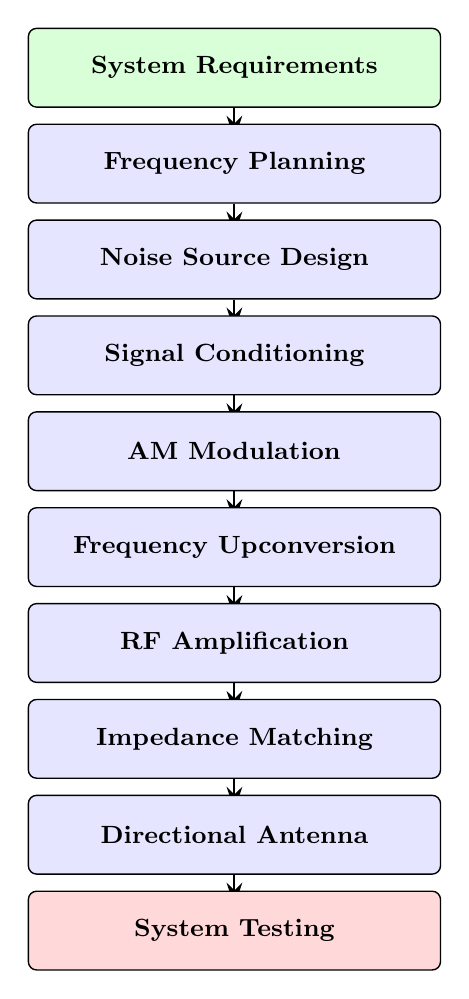
\begin{tikzpicture}[
			node distance=0.6cm,
			block/.style={
				rectangle,
				draw,
				fill=blue!10,
				text width=5cm,
				text centered,
				minimum height=1cm,
				rounded corners=3pt,
				font=\small\bfseries,
				line width=0.5pt
			},
			arrow/.style={
				-{Stealth[length=3mm, width=2mm]},
				thick,
				line width=0.7pt
			}
			]
			
			% Block 1: System Requirements
			\node[block, fill=green!15] (req) {System Requirements};
			
			\draw[arrow] (req.south) -- ++(0,-0.4);
			
			% Block 2: Frequency Planning
			\node[block, below=0.2cm of req] (freq) {Frequency Planning};
			
			\draw[arrow] (freq.south) -- ++(0,-0.4);
			
			% Block 3: Noise Source Design
			\node[block, below=0.2cm of freq] (noise) {Noise Source Design};
			
			\draw[arrow] (noise.south) -- ++(0,-0.4);
			
			% Block 4: Signal Conditioning
			\node[block, below=0.2cm of noise] (cond) {Signal Conditioning};
			
			\draw[arrow] (cond.south) -- ++(0,-0.4);
			
			% Block 5: AM Modulation
			\node[block, below=0.2cm of cond] (am) {AM Modulation};
			
			\draw[arrow] (am.south) -- ++(0,-0.4);
			
			% Block 6: Frequency Upconversion
			\node[block, below=0.2cm of am] (upconv) {Frequency Upconversion};
			
			\draw[arrow] (upconv.south) -- ++(0,-0.4);
			
			% Block 7: RF Amplification
			\node[block, below=0.2cm of upconv] (amp) {RF Amplification};
			
			\draw[arrow] (amp.south) -- ++(0,-0.4);
			
			% Block 8: Impedance Matching
			\node[block, below=0.2cm of amp] (match) {Impedance Matching};
			
			\draw[arrow] (match.south) -- ++(0,-0.4);
			
			% Block 9: Directional Antenna
			\node[block, below=0.2cm of match] (ant) {Directional Antenna};
			
			\draw[arrow] (ant.south) -- ++(0,-0.4);
			
			% Block 10: System Testing
			\node[block, fill=red!15, below=0.2cm of ant] (test) {System Testing};
			
		\end{tikzpicture}
		\caption{System Design Flowchart}
		\label{fig:system_flow}
	\end{figure}
	
	\subsection{Design Requirements}
	The overall system specifications were established before the hardware design commenced. 
	\begin{table}[htbp]
		\centering
		\caption{System Design Parameters}
		\label{tab:design_parameters}
		\begin{tabular}{p{5cm} p{5cm}}
			\toprule
			\textbf{Parameter} & \textbf{Design Value} \\
			\midrule
			Operating Band & 2.4 GHz ISM \\
			Second Operating Band & 5.8 GHz ISM \\
			Supply Voltage & 12 V DC \\
			Noise Source & 6.8 V Zener Diode \\
			Carrier Frequency & 1 kHz \\
			Mixer & ADE-30 Double Balanced Mixer \\
			Local Oscillator & MS-3000 VCO \\
			RF Amplifier & RF2126 \\
			Antenna Gain & 11 $\pm$1 dBi \\
			Impedance & 50 $\Omega$ \\
			Polarization & Linear Vertical \\
			VSWR & 1.92 : 1 \\
			\bottomrule
		\end{tabular}
	\end{table}
	
	The operating frequency bands were selected because they are widely used for Wi-Fi, Bluetooth, industrial wireless communication, and other ISM-band applications, making them suitable for laboratory research and RF system analysis.
	
	
	\subsection{Design Assumptions}
	
	To simplify the engineering analysis and mathematical modeling, several assumptions were adopted during the design process.
	
	\subsubsection*{Constant Supply Voltage}
	
	The DC power supply is assumed to remain constant at
	\begingroup
	\setlength{\mathindent}{0pt}
	\begin{equation}
		V_{CC} = 12\ \text{V}
	\end{equation}
	\endgroup
	without ripple or transient fluctuations.
	
	\subsubsection*{Constant Characteristic Impedance}
	
	Every RF component in the transmitter chain is assumed to operate with a characteristic impedance of
	\begin{equation}
		Z_0 = 50\ \Omega
	\end{equation}
	This assumption ensures maximum power transfer and minimizes signal reflections throughout the RF chain.
	
	\subsubsection*{Stable Local Oscillator}
	
	The MS-3000 Voltage Controlled Oscillator is assumed to generate a stable sinusoidal output with negligible frequency drift during system operation. The Local Oscillator signal is represented as
	\begin{equation}
		V_{LO} = A_{LO} \cos(2\pi f_{LO} t)
	\end{equation}
	where
	\begin{align*}
		A_{LO} &= \text{LO amplitude} \\
		f_{LO} &= \text{LO frequency}
	\end{align*}
	
	\subsubsection*{Random Noise Source}
	
	The avalanche noise generated by the Zener diode is assumed to possess a zero mean
	\begin{equation}
		E[n(t)] = 0
	\end{equation}
	and a Gaussian amplitude distribution over the useful bandwidth.
	
	\subsubsection*{Linear Operation}
	
	The RF amplifier is assumed to operate within its linear region. Therefore,
	\begin{equation}
		P_{out} = G \times P_{in}
	\end{equation}
	where $G$ denotes amplifier gain. Nonlinear distortion and harmonic generation are neglected during first-order analysis.
	
		
	\subsection{Frequency Planning}
	One of the most critical stages of RF system design is frequency planning. Proper frequency planning ensures that the desired RF signal appears at the required output while minimizing image frequencies and unwanted mixer products.
	
	The ADE-30 is a passive double-balanced mixer that generates both sum and difference frequencies according to
	\begin{equation}
		f_{RF} = f_{LO} \pm f_{IF}
	\end{equation}
	
	The mixer exhibits a typical conversion loss of approximately 4.5--6 dB and is designed for an optimum +7 dBm LO drive, making it suitable for ISM-band frequency conversion.
	
	For operation in the 2.4 GHz band:
	\begin{align*}
		f_{LO} &= 2.450\ \text{GHz} \\
		f_{IF} &= 1\ \text{kHz}
	\end{align*}
	
	Therefore,
	\begin{equation}
		f_{RF} = 2.450\ \text{GHz} \pm 1\ \text{kHz}
	\end{equation}
	
	Since
	\begin{equation}
		1\ \text{kHz} \ll 2.45\ \text{GHz}
	\end{equation}
	the translated RF signal remains effectively centered at 2.45 GHz.
	
	Similarly, for the 5.8 GHz mode,
	\begin{equation}
		f_{LO} = 5.800\ \text{GHz}
	\end{equation}
	
	Hence,
	\begin{equation}
		f_{RF} = 5.800\ \text{GHz} \pm 1\ \text{kHz}
	\end{equation}
	which remains centered at 5.8 GHz.
	
	This frequency planning enables simple switching between both ISM bands while maintaining identical IF circuitry.
	
	
	\subsection{Impedance Planning}
	Impedance mismatch is one of the major causes of RF power loss. Therefore, every subsystem was designed around the industry-standard $50\ \Omega$ RF environment. The following components all employ $50\ \Omega$ interfaces:
	\begin{itemize}
		\item ADE-30 Mixer
		\item RF2126 Amplifier
		\item SMA Connectors
		\item RF Coaxial Cable
		\item Directional Antenna
	\end{itemize}
	Maintaining identical impedance throughout the RF chain minimizes reflections and standing waves.
	
	The reflection coefficient is
	\begin{equation}
		\Gamma = \frac{Z_L - Z_0}{Z_L + Z_0}
	\end{equation}
	where
	\begin{align*}
		Z_L &= \text{Load impedance} \\
		Z_0 &= \text{Characteristic impedance}
	\end{align*}
	
	When
	\begin{equation}
		Z_L = 50\ \Omega
	\end{equation}
	and
	\begin{equation}
		Z_0 = 50\ \Omega
	\end{equation}
	then
	\begin{equation}
		\Gamma = 0
	\end{equation}
	which indicates perfect impedance matching and zero reflected power.
	
	\subsection{Power Budget Planning}
	A preliminary power budget was established to estimate the RF signal level throughout the transmitter chain.
	
	Assume:
	\begin{align*}
		P_{Mixer} &= 0\ \text{dBm} && \text{(Mixer Output)} \\
		L_c &= 6\ \text{dB} && \text{(ADE-30 Conversion Loss)}
	\end{align*}
	
	Therefore,
	\begin{equation}
		P_{AfterMixer} = 0 - 6 = -6\ \text{dBm}
	\end{equation}
	
	If the RF2126 amplifier provides
	\begin{equation}
		G = 20\ \text{dB}
	\end{equation}
	then
	\begin{equation}
		P_{Output} = -6 + 20 = 14\ \text{dBm}
	\end{equation}
	
	This power budget demonstrates the necessity of the RF amplifier to compensate for the passive mixer's conversion loss and increase the transmitted RF power.
	\subsection{Design Verification Strategy}
	
	The verification sequence included the following:
	
	\subsubsection{Noise Source Verification}
	\begin{itemize}
		\item Verify breakdown voltage.
		\item Watch random noise with oscilloscope.
	\end{itemize}
	
	\subsubsection{Signal Conditioning Verification}
	\begin{itemize}
		\item Verify DC block.
		\item Measure AC coupling.
	\end{itemize}
	
	\subsubsection{AM Modulator Verification}
	\begin{itemize}
		\item Verify presence of upper and lower sidebands.
		\item Assess modulation depth.
	\end{itemize}
	
	\subsubsection{Mixer Verification}
	\begin{itemize}
		\item Apply required LO drive.
		\item Measure frequency of RF output.
		\item Measure conversion loss and port isolation.
	\end{itemize}
	
	\subsubsection{RF Amplifier Verification}
	\begin{itemize}
		\item Measure gain.
		\item Assess output power.
		\item Verify amplifier stability.
	\end{itemize}
	
	\subsubsection{Antenna Verification}
	\begin{itemize}
		\item Measure VSWR.
		\item Verify impedance matching.
		\item Observe radiation characteristics.
	\end{itemize}
	\subsection{Component Selection Methodology}
	RF system hardware design and components: One of the biggest steps in designing an RF system design is selecting all the right hardware parts, as the performance of a transmitter depends directly on the properties of its components. In this paper, the dual band RF interference system was constructed by using a set of commercially available RF components, which fulfills the frequency, physical and electrical specifications for the project. Criteria such as the following were considered in the selection process of components:
	
	\begin{itemize}
		\item frequency matching,
		\item impedance matching,
		\item power rating,
		\item noise figures,
		\item gain,
		\item physical dimensions,
		\item availability,
		\item cost,
		\item reliability,
		\item ease of PCB implementation,
	\end{itemize}
	
	Each component was picked by studying their datasheets and compatibility with the other RF system components.
		
	\subsubsection{Selection of the Zener Diode}
	
	The interference signal originates from a 6.8 V Zener diode operated in reverse avalanche breakdown. A 6.8 V Zener diode was selected because it provides:
	\begin{itemize}
		\item Stable avalanche operation
		\item Significant broadband noise generation
		\item Good thermal stability
		\item Low cost
		\item Easy availability
		\item Simple biasing
	\end{itemize}
	The reverse-biased junction generates random charge-carrier multiplication, producing broadband electrical noise suitable for analog RF interference applications.
	
	The Zener voltage satisfies
	\begingroup
	\setlength{\mathindent}{0pt}
	\begin{equation*}
		\hfill
		V_Z = 6.8\ \text{V}
		\hfill
	\end{equation*}
	\endgroup
	while the applied supply voltage is
	\begingroup
	\setlength{\mathindent}{0pt}
	\begin{equation*}
		\hfill
		V_{CC} = 12\ \text{V}
		\hfill
	\end{equation*}
	\endgroup
	Therefore the diode always remains in avalanche mode.
	
	\subsubsection{Selection of the Bias Resistor}
	
	The resistor determines the avalanche current flowing through the Zener diode. Using Ohm's Law,
	\begingroup
	\setlength{\mathindent}{0pt}
	\begin{equation*}
		\hfill
		R = \frac{V_{CC} - V_Z}{I_Z}
		\hfill
	\end{equation*}
	\endgroup
	
	Assuming
	\begingroup
	\setlength{\mathindent}{0pt}
	\begin{equation*}
		\hfill
		V_{CC} = 12\ \text{V}
		\hfill
	\end{equation*}
	\endgroup
	\begingroup
	\setlength{\mathindent}{0pt}
	\begin{equation*}
		\hfill
		V_Z = 6.8\ \text{V}
		\hfill
	\end{equation*}
	\endgroup
	
	Desired current
	\begingroup
	\setlength{\mathindent}{0pt}
	\begin{equation*}
		\hfill
		I_Z = 10\ \text{mA}
		\hfill
	\end{equation*}
	\endgroup
	
	Therefore
	\begingroup
	\setlength{\mathindent}{0pt}
	\begin{equation*}
		\hfill
		R = \frac{12 - 6.8}{0.01} = 520\ \Omega
		\hfill
	\end{equation*}
	\endgroup
	
	The nearest standard value is
	\begingroup
	\setlength{\mathindent}{0pt}
	\begin{equation*}
		\hfill
		560\ \Omega
		\hfill
	\end{equation*}
	\endgroup
	
	The resistor also limits current and protects the diode from excessive power dissipation.
	
	\subsubsection{Selection of the Coupling Capacitor}
	
	The output of the avalanche diode contains both
	\begin{itemize}
		\item DC component
		\item AC noise
	\end{itemize}
	Only the AC component should propagate toward the modulator. Therefore, a
	\begingroup
	\setlength{\mathindent}{0pt}
	\begin{equation*}
		\hfill
		0.1\ \mu\text{F}
		\hfill
	\end{equation*}
	\endgroup
	capacitor was selected.
	
	Its reactance is
	\begingroup
	\setlength{\mathindent}{0pt}
	\begin{equation*}
		\hfill
		X_C = \frac{1}{2\pi fC}
		\hfill
	\end{equation*}
	\endgroup
	
	For
	\begingroup
	\setlength{\mathindent}{0pt}
	\begin{equation*}
		\hfill
		f = 1\ \text{kHz}
		\hfill
	\end{equation*}
	\endgroup
	and
	\begingroup
	\setlength{\mathindent}{0pt}
	\begin{equation*}
		\hfill
		C = 0.1\ \mu\text{F}
		\hfill
	\end{equation*}
	\endgroup
	
	\begingroup
	\setlength{\mathindent}{0pt}
	\begin{equation*}
		\hfill
		X_C = \frac{1}{2\pi(1000)(0.1 \times 10^{-6})} = 1591\ \Omega
		\hfill
	\end{equation*}
	\endgroup
	
	At higher noise frequencies the reactance decreases further, allowing broadband noise to pass while blocking DC.
	
	\subsubsection{Selection of ADE-30 Mixer}
	
	The frequency conversion stage requires a mixer with:
	\begin{itemize}
		\item Wide RF bandwidth
		\item Low conversion loss
		\item High port isolation
		\item Standard 50 $\Omega$ impedance
		\item Low insertion loss
		\item Simple PCB implementation
	\end{itemize}
	The ADE-30 passive double-balanced mixer satisfies these requirements.
	
	Typical characteristics include:
	
	\begin{table}[htbp]
		\centering
		\begin{tabular}{p{5cm} p{5cm}}
			\toprule
			\textbf{Parameter} & \textbf{Typical Value} \\
			\midrule
			Frequency Range & 200 MHz--3 GHz \\
			LO Drive & +7 dBm \\
			Conversion Loss & 4.5--6 dB \\
			LO-RF Isolation & $\approx$35 dB \\
			Impedance & 50 $\Omega$ \\
			\bottomrule
		\end{tabular}
		\caption{ADE-30 Typical Characteristics}
		\label{tab:ade30}
	\end{table}
	
	These characteristics make the device well suited for ISM-band frequency translation and laboratory RF systems.
	
	\subsubsection{Selection of MS-3000 VCO}
	
	The Local Oscillator determines the RF output frequency. The VCO was selected because it provides:
	\begin{itemize}
		\item Continuous frequency tuning
		\item Good frequency stability
		\item Microwave-frequency operation
		\item Compact construction
		\item Stable sinusoidal output
	\end{itemize}
	The oscillator supplies the required LO signal to the ADE-30 mixer. The LO waveform is
	\begingroup
	\setlength{\mathindent}{0pt}
	\begin{equation*}
		\hfill
		V_{LO} = A_{LO} \cos(2\pi f_{LO} t)
		\hfill
	\end{equation*}
	\endgroup
	where
	\begingroup
	\setlength{\mathindent}{0pt}
	\begin{equation*}
		\hfill
		f_{LO} = 2.45\ \text{GHz}
		\hfill
	\end{equation*}
	\endgroup
	or
	\begingroup
	\setlength{\mathindent}{0pt}
	\begin{equation*}
		\hfill
		5.80\ \text{GHz}
		\hfill
	\end{equation*}
	\endgroup
	depending on the operating mode.
	
	\subsubsection{Selection of RF2126 Power Amplifier}
	
	Passive mixers inherently introduce conversion loss. Consequently, an RF amplifier is required to restore the RF power before antenna transmission. The RF2126 amplifier was selected because it offers:
	\begin{itemize}
		\item High RF gain
		\item Stable microwave operation
		\item Good linearity
		\item Low power consumption
		\item Compatibility with 50 $\Omega$ systems
		\item Compact PCB footprint
	\end{itemize}
	The amplifier compensates for the conversion loss introduced by the mixer and increases the transmitted RF power.
	
	If
	\begingroup
	\setlength{\mathindent}{0pt}
	\begin{equation*}
		\hfill
		P_{IN} = -6\ \text{dBm} \quad \text{(Mixer Output)}
		\hfill
	\end{equation*}
	\endgroup
	
	Amplifier Gain
	\begingroup
	\setlength{\mathindent}{0pt}
	\begin{equation*}
		\hfill
		G = 20\ \text{dB}
		\hfill
	\end{equation*}
	\endgroup
	
	Then
	\begingroup
	\setlength{\mathindent}{0pt}
	\begin{equation*}
		\hfill
		P_{OUT} = -6 + 20 = 14\ \text{dBm}
		\hfill
	\end{equation*}
	\endgroup
	
	This amplification significantly increases the transmitted field strength.
	
	\subsubsection{Selection of Directional Antenna}
	
	The antenna represents the final RF subsystem. The selected antenna possesses
	
	\begin{table}[htbp]
		\centering
		\begin{tabular}{p{5cm} p{5cm}}
			\toprule
			\textbf{Parameter} & \textbf{Value} \\
			\midrule
			Gain & 11 $\pm$1 dBi \\
			VSWR & 1.92:1 \\
			Polarization & Linear Vertical \\
			Impedance & 50 $\Omega$ \\
			\bottomrule
		\end{tabular}
		\caption{Antenna Specifications}
		\label{tab:antenna_specs}
	\end{table}
	
	The directional radiation pattern concentrates transmitted power into a narrow beam.
	
	The wavelength for 2.45 GHz is
	\begingroup
	\setlength{\mathindent}{0pt}
	\begin{equation*}
		\hfill
		\lambda = \frac{3 \times 10^8}{2.45 \times 10^9} = 0.122\ \text{m} = 12.2\ \text{cm}
		\hfill
	\end{equation*}
	\endgroup
	
	Similarly, for 5.8 GHz
	\begingroup
	\setlength{\mathindent}{0pt}
	\begin{equation*}
		\hfill
		\lambda = \frac{3 \times 10^8}{5.8 \times 10^9} = 0.0517\ \text{m} = 5.17\ \text{cm}
		\hfill
	\end{equation*}
	\endgroup
	
	These wavelengths directly influence antenna dimensions and spacing.
	
		
	\subsection{Engineering Design Constraints}
	
	During the design process several engineering constraints were identified and addressed.
	
	\subsubsection{Power Limitation}
	
	The entire transmitter operates from a single 12 V DC supply. Therefore every subsystem must satisfy
	\begingroup
	\setlength{\mathindent}{0pt}
	\begin{equation*}
		\hfill
		P = VI
		\hfill
	\end{equation*}
	\endgroup
	without exceeding the available power budget.
	
	\subsubsection{Impedance Matching}
	
	Every RF subsystem was designed for 50 $\Omega$ operation. Impedance mismatch causes
	\begin{itemize}
		\item reflected power
		\item standing waves
		\item reduced amplifier efficiency
	\end{itemize}
	
	The return loss is
	\begingroup
	\setlength{\mathindent}{0pt}
	\begin{equation*}
		\hfill
		RL = -20\log|\Gamma|
		\hfill
	\end{equation*}
	\endgroup
	where
	\begingroup
	\setlength{\mathindent}{0pt}
	\begin{equation*}
		\hfill
		\Gamma = \frac{Z_L - Z_0}{Z_L + Z_0}
		\hfill
	\end{equation*}
	\endgroup
	
	Perfect matching gives
	\begingroup
	\setlength{\mathindent}{0pt}
	\begin{equation*}
		\hfill
		RL \rightarrow \infty
		\hfill
	\end{equation*}
	\endgroup
	while practical RF systems generally consider return losses better than about 10 dB acceptable, with higher values indicating improved matching.
	
	\subsubsection{PCB Layout}
	
	At microwave frequencies, PCB traces behave as transmission lines. Consequently,
	\begin{itemize}
		\item trace length
		\item trace width
		\item dielectric constant
		\item ground plane continuity
	\end{itemize}
	all influence RF performance. Transmission-line effects become increasingly important at gigahertz frequencies, requiring controlled-impedance routing and careful layout practices.
	
	\subsubsection{Thermal Management}
	
	The RF amplifier dissipates power during operation. Therefore, adequate copper area, proper grounding, and sufficient heat sinking must be provided to prevent thermal instability.
	
	\subsection{Summary}
	In this chapter, the design methodology of a dual band directional RF interference system was introduced. The system is divided into following module using a modular analog RF structure, which is Avalanche noise source, Signal conditioning network, Amplitude modulation section, Frequency up conversion by means of ADE-30 mixer and MS-3000 VCO, RF power amplification by means of RF2126 amplifier, and Directional transmission with 50-high gain antenna. These components were chosen and justified with consideration of electrical characteristics, impedance matching, frequency range, system integration requirement and their application in the project. 
	
	Moreover, impedance matching, PCB layout, power budget and thermal management are also designed constraints that we took into account to make sure system reliable. 
	
	In following chapter (3.2 Design of the Project Hardware/Software), we will go deeper into the detail of each module and discuss their detailed circuit design, mathematical equation, engineering calculation, size selection of components, and hardware implement process of the system.
	
	\section{Design of the Project Hardware/Software }
	
	\subsection{Introduction}
	The overall system methodology described in Section 3.1 has been used to create the detailed engineering design of each subsystem used for the dual-band directional RF interference generator. Unlike Section 3.1 which describes the overall system architecture and methodology, this section presents the electrical design, component selection, mathematical calculation and hardware implementation of each functional block. The proposed system has been designed using a modular RF transmitter architecture, where each stage in the system has a specific signal processing task to perform.
	
	The signal starts at the avalanche noise source (broadband) and then proceeds through signal conditioning, amplitude modulation, microwave frequency up-conversion, RF power amplifier and finally radiated through a high-gain directional antenna.
	
	The entire RF chain consists of the following hardware modules:
	\begin{enumerate}
		\item Avalanche Noise Generator
		\item Signal Conditioning Circuit
		\item Amplitude Modulator
		\item ADE-30 Double-Balanced Mixer
		\item MS-3000 Voltage Controlled Oscillator (VCO)
		\item RF2126 High-Power RF Amplifier
		\item High-Gain Directional Antenna
	\end{enumerate}
	
	All these modules were designed individually and integrated to obtain the final transmitter. This approach has the following benefits:
	\begin{itemize}
		\item Allows testing of all subsystems individually
		\item Easy fault diagnosis
		\item Simple maintenance
		\item Flexible design
		\item Simple implementation
		\item High reliability
	\end{itemize}
	
	The details of each subsystem will be described in the subsequent sections.
	
	\subsection{Design of Avalanche Noise Generator}
	
	\subsubsection{Introduction}
	The avalanche noise generator is the main signal source in the proposed RF interference system. The Avalanche Noise Generator produces a random electrical noise of broadband characteristics which will serve as the message signal when amplitude modulated. Unlike ordinary oscillations from deterministic oscillators, this avalanche noise is generated from the micro collision of the carriers in the interior of a reverse-biased semiconductor junction.
	
	The carriers are energized and obtain enough kinetic energy to generate new carriers when the reverse bias voltage surpasses the avalanche breakdown voltage by the impact ionization phenomenon.
	
	Due to the nature of statistically random fluctuations and its broadband spectrum, Avalanche Noise has been a common source of noise for various RF test systems, communication testing, and laboratory test signals. A 6.8V Zener Diode is used in the design because this reverse voltage value ensures that the Zener diode operates in the avalanche region, and this has the simplest form in the operating circuit of avalanche noise generator.
	
	\subsubsection{Principle of Avalanche Breakdown}
	A reverse biased junction develops a depletion layer and increases until a critical value of electric field across it is reached, at which the charge carriers accelerated through it collide with atoms and create new carriers through the impact ionization mechanism. The process of multiplication occurs in a random way leading to broadband electrical noise.
	
	The avalanche multiplication factor $M$ is described by the formula:
	\begingroup
	\setlength{\mathindent}{0pt}
	\begin{equation*}
		\hfill
		M = \frac{1}{1 - \left(\frac{V_R}{V_{BR}}\right)^n}
		\hfill
	\end{equation*}
	\endgroup
	where
	\begin{align*}
		M &= \text{Avalanche multiplication factor} \\
		V_R &= \text{Applied reverse voltage} \\
		V_{BR} &= \text{Breakdown voltage} \\
		n &= \text{Empirical constant which depends on the junction}
	\end{align*}
	
	\subsubsection{Circuit Design}
	The components needed for the avalanche noise generator are:
	\begin{enumerate}
		\item 12V stabilized DC supply
		\item 560-ohm series resistor
		\item 6.8V Zener diode
		\item 0.1 $\mu$F coupling capacitor
	\end{enumerate}
	\begin{figure}[htbp]
		\centering
		\begin{circuitikz}[american]
			\draw
			% Power supply
			(0,0) node[above] {$+12V$} to[short, o-] (0,0)
			% Resistor
			to[R, l=$560\Omega$, o-] (0,-2)
			% Node
			(0,-2) to[short, -*] (2.5,-2)
			% Output
			(2.5,-2) to[short, -o] (3.5,-2) node[right] {Output}
			% Zener diode
			(0,-2) to[full diode, l=$6.8V$ Zener, invert] (0,-4.5)
			% Ground
			(0,-4.5) node[ground] {}
			;
		\end{circuitikz}
		\caption{Simplified Zener Noise Generator Circuit}
		\label{fig:zener_circuit}
	\end{figure}
	
	The resistor placed in series with the Zener diode allows the same to function at avalanche level, preventing over-voltage.
	
	\subsubsection{Design of the Biasing Resistor}
	The value of the resistor is calculated based on the desired avalanche current. According to Ohm's law:
	\begingroup
	\setlength{\mathindent}{0pt}
	\begin{equation*}
		\hfill
		R = \frac{V_{CC} - V_Z}{I_Z}
		\hfill
	\end{equation*}
	\endgroup
	where
	\begin{align*}
		V_{CC} &= 12\ \text{V} \\
		V_Z &= 6.8\ \text{V} \\
		I_Z &= 10\ \text{mA} \quad (\text{Desired current})
	\end{align*}
	
	Substitute the values:
	\begingroup
	\setlength{\mathindent}{0pt}
	\begin{equation*}
		\hfill
		R = \frac{12 - 6.8}{0.01} = \frac{5.2}{0.01} = 520\ \Omega
		\hfill
	\end{equation*}
	\endgroup
	
	Since 520 $\Omega$ is not a preferred resistor value, we choose the nearest standard value, which is $560\ \Omega$.
	
	With $R = 560\ \Omega$, the actual Zener current becomes:
	\begingroup
	\setlength{\mathindent}{0pt}
	\begin{equation*}
		\hfill
		I_Z = \frac{12 - 6.8}{560} = \frac{5.2}{560} = 9.29\ \text{mA}
		\hfill
	\end{equation*}
	\endgroup
	
	This operating current is close to our target value and ensures that the diode operates in the avalanche region safely.
	
	\subsubsection{Power Dissipation Analysis}
	Power dissipated by the resistor is:
	\begingroup
	\setlength{\mathindent}{0pt}
	\begin{equation*}
		\hfill
		P_R = I^2R = (9.29 \times 10^{-3})^2 \times 560 = 0.048\ \text{W}
		\hfill
	\end{equation*}
	\endgroup
	
	A 0.25 W resistor will suffice with a comfortable margin.
	
	Power dissipated by the Zener diode is:
	\begingroup
	\setlength{\mathindent}{0pt}
	\begin{equation*}
		\hfill
		P_Z = V_Z I_Z = 6.8 \times 9.29 \times 10^{-3} = 0.063\ \text{W}
		\hfill
	\end{equation*}
	\endgroup
	
	The diode dissipates only 63 mW, which is well below the rating of a typical 6.8 V Zener diode (often around 500 mW).
	\subsubsection{Small-Signal Noise Considerations}
	The avalanche noise produced by the reverse-biased Zener diode can be represented as a broadband random voltage source added to the DC bias. The instantaneous output voltage is:
	\begingroup
	\setlength{\mathindent}{0pt}
	\begin{equation*}
		\hfill
		v(t) = V_Z + n(t)
		\hfill
	\end{equation*}
	\endgroup
	where
	\begin{align*}
		V_Z &= \text{DC Zener voltage} \\
		n(t) &= \text{Random noise voltage}
	\end{align*}
	
	After coupling to the AC stage, the DC component is blocked and we are left with the noise signal:
	\begingroup
	\setlength{\mathindent}{0pt}
	\begin{equation*}
		\hfill
		v_{out}(t) = n(t)
		\hfill
	\end{equation*}
	\endgroup
	
	This signal serves as the input to the amplitude modulation stage. The noise power is related to the RMS noise voltage by:
	\begingroup
	\setlength{\mathindent}{0pt}
	\begin{equation*}
		\hfill
		P_n = \frac{V_{n,RMS}^2}{R}
		\hfill
	\end{equation*}
	\endgroup
	where $R$ is the load impedance. For a matched RF system, $R = 50\ \Omega$. The available noise power can be calculated if $V_{n,RMS}$ is measured.
	
	\subsubsection{Design Considerations}
	Several aspects were considered to ensure a stable and repeatable noise source:
	\begin{enumerate}
		\item \textbf{Stable Supply:} A regulated 12V DC supply is used to ensure constant current flow through the Zener diode, leading to stable avalanche current and noise levels.
		\item \textbf{Current Limiting:} The $560\ \Omega$ resistor limits the Zener current to a safe operating level while keeping it within the avalanche region.
		\item \textbf{Thermal Stability:} The low power dissipation (63 mW) by the Zener diode minimizes the impact of temperature variations on its performance.
		\item \textbf{Isolation:} The output is AC-coupled to avoid introducing DC bias into the following AM modulator.
		\item \textbf{Physical Layout:} The Zener diode and biasing resistor should be placed close together, with short traces and a good ground plane, to minimize stray inductance and susceptibility to external interference in RF circuits.
	\end{enumerate}
	\subsection{Design of the Signal Conditioning Circuit}
	
	\subsubsection{Introduction}
	A reverse-biased Zener diode operating in avalanche mode generates both a DC voltage equal to the Zener voltage and a broadband AC noise component. In the context of an RF interference system utilizing avalanche noise for AM, the AC noise component is the only useful signal. Thus, a signal-conditioning circuit is required immediately after the noise generator to extract and pass only this AC noise to the subsequent amplitude modulator.
	
	The primary functions of this signal conditioning circuit are to:
	\begin{itemize}
		\item Block the DC bias of the Zener diode.
		\item Pass the broadband avalanche noise with minimal attenuation and spectral distortion.
		\item Prevent any DC offset from reaching the amplitude modulator.
		\item Ensure the overall signal integrity for effective modulation.
	\end{itemize}
	
	The chosen signal conditioning circuit is a simple series coupling capacitor. A $0.1\ \mu$F ceramic coupling capacitor (marked as 104) is used, connecting the avalanche noise source to the AM modulator.
	\subsubsection{Operating Principle of the Coupling Capacitor}
	A capacitor behaves as a frequency-dependent impedance, known as capacitive reactance ($X_C$). For DC signals (frequency = 0), the reactance is infinite, blocking current flow. As the signal frequency increases, the reactance decreases, allowing more AC current to pass. The relationship is given by:
	\begingroup
	\setlength{\mathindent}{0pt}
	\begin{equation*}
		\hfill
		X_C = \frac{1}{2\pi fC}
		\hfill
	\end{equation*}
	\endgroup
	where
	\begin{align*}
		X_C &= \text{Capacitive reactance } (\Omega) \\
		f &= \text{Signal frequency (Hz)} \\
		C &= \text{Capacitance (F)}
	\end{align*}
	
	This inversely proportional relationship with frequency makes the coupling capacitor effective in passing AC signals while blocking DC. In RF applications, it's important that the capacitor has low reactance at the desired signal frequencies and is placed close to the stages it connects to minimize stray inductance and parasitic effects.
	
	\subsubsection{Capacitor Selection}
	The coupling capacitor selected for this design is:
	\begingroup
	\setlength{\mathindent}{0pt}
	\begin{equation*}
		\hfill
		C = 0.1\ \mu\text{F} = 100\ \text{nF} = 1 \times 10^{-7}\ \text{F}
		\hfill
	\end{equation*}
	\endgroup
	
	A $0.1\ \mu$F ceramic capacitor is a suitable choice for this application due to its:
	\begin{itemize}
		\item Excellent high-frequency performance (low impedance).
		\item Low equivalent series resistance (ESR) and equivalent series inductance (ESL).
		\item Good temperature stability and reliability.
		\item Compact size and low cost.
		\item Wide availability and general suitability for RF coupling.
	\end{itemize}
	
	Ceramic capacitors are a preferred choice in RF circuits due to their favorable impedance characteristics across a wide range of frequencies and minimal parasitic effects.
	\subsubsection{Capacitive Reactance Analysis}
	To evaluate the capacitor behavior at different frequencies, the reactance is calculated using
	\begingroup
	\setlength{\mathindent}{0pt}
	\begin{equation*}
		\hfill
		X_C = \frac{1}{2\pi fC}
		\hfill
	\end{equation*}
	\endgroup
	
	\subsubsection*{At 1 kHz}
	\begingroup
	\setlength{\mathindent}{0pt}
	\begin{equation*}
		\hfill
		X_C = \frac{1}{2\pi(1000)(0.1 \times 10^{-6})}
		\hfill
	\end{equation*}
	\endgroup
	\begingroup
	\setlength{\mathindent}{0pt}
	\begin{equation*}
		\hfill
		X_C = 1591.5\ \Omega
		\hfill
	\end{equation*}
	\endgroup
	
	\subsubsection*{At 10 kHz}
	\begingroup
	\setlength{\mathindent}{0pt}
	\begin{equation*}
		\hfill
		X_C = \frac{1}{2\pi(10000)(0.1 \times 10^{-6})}
		\hfill
	\end{equation*}
	\endgroup
	\begingroup
	\setlength{\mathindent}{0pt}
	\begin{equation*}
		\hfill
		X_C = 159.15\ \Omega
		\hfill
	\end{equation*}
	\endgroup
	
	\subsubsection*{At 100 kHz}
	\begingroup
	\setlength{\mathindent}{0pt}
	\begin{equation*}
		\hfill
		X_C = 15.9\ \Omega
		\hfill
	\end{equation*}
	\endgroup
	
	\subsubsection*{At 1 MHz}
	\begingroup
	\setlength{\mathindent}{0pt}
	\begin{equation*}
		\hfill
		X_C = 1.59\ \Omega
		\hfill
	\end{equation*}
	\endgroup
	
	\subsubsection*{At 10 MHz}
	\begingroup
	\setlength{\mathindent}{0pt}
	\begin{equation*}
		\hfill
		X_C = 0.159\ \Omega
		\hfill
	\end{equation*}
	\endgroup
	
	\subsubsection*{At 100 MHz}
	\begingroup
	\setlength{\mathindent}{0pt}
	\begin{equation*}
		\hfill
		X_C = 0.0159\ \Omega
		\hfill
	\end{equation*}
	\endgroup
	
	\subsubsection*{Summary Table}
	
	\begin{table}[htbp]
		\centering
		\caption{Capacitive Reactance at Different Frequencies}
		\label{tab:reactance}
		\begin{tabular}{p{5cm} p{5cm}}
			\toprule
			\textbf{Frequency} & \textbf{Capacitive Reactance} \\
			\midrule
			1 kHz & 1591.5 $\Omega$ \\
			10 kHz & 159.15 $\Omega$ \\
			100 kHz & 15.9 $\Omega$ \\
			1 MHz & 1.59 $\Omega$ \\
			10 MHz & 0.159 $\Omega$ \\
			100 MHz & 0.0159 $\Omega$ \\
			\bottomrule
		\end{tabular}
	\end{table}
	
	These results clearly show that the impedance decreases rapidly with increasing frequency. Therefore, the broadband high-frequency components of the avalanche noise are transferred to the next stage with negligible attenuation, while the DC component remains blocked.
	
	
	\subsubsection{High-Pass Filter Analysis}
	The coupling capacitor and the input resistance of the following stage form a first-order RC high-pass filter. The cut-off frequency is
	\begingroup
	\setlength{\mathindent}{0pt}
	\begin{equation*}
		\hfill
		f_c = \frac{1}{2\pi RC}
		\hfill
	\end{equation*}
	\endgroup
	where
	\begin{align*}
		R &= \text{Input resistance of the next stage} \\
		C &= \text{Coupling capacitance}
	\end{align*}
	
	Assuming the AM modulator presents an input resistance of
	\begingroup
	\setlength{\mathindent}{0pt}
	\begin{equation*}
		\hfill
		R = 10\ \text{k}\Omega
		\hfill
	\end{equation*}
	\endgroup
	then
	\begingroup
	\setlength{\mathindent}{0pt}
	\begin{equation*}
		\hfill
		f_c = \frac{1}{2\pi(10000)(0.1 \times 10^{-6})}
		\hfill
	\end{equation*}
	\endgroup
	\begingroup
	\setlength{\mathindent}{0pt}
	\begin{equation*}
		\hfill
		f_c = 159.15\ \text{Hz}
		\hfill
	\end{equation*}
	\endgroup
	
	This cut-off frequency is well below the frequencies of interest, ensuring that the useful signal passes while the DC component is rejected. The same relationship is widely used for AC-coupling networks in analog circuits.
	
	\subsubsection{Time Constant Analysis}
	The RC time constant determines how quickly the capacitor charges and discharges. It is given by
	\begingroup
	\setlength{\mathindent}{0pt}
	\begin{equation*}
		\hfill
		\tau = RC
		\hfill
	\end{equation*}
	\endgroup
	
	Substituting
	\begingroup
	\setlength{\mathindent}{0pt}
	\begin{equation*}
		\hfill
		R = 10\ \text{k}\Omega
		\hfill
	\end{equation*}
	\endgroup
	\begingroup
	\setlength{\mathindent}{0pt}
	\begin{equation*}
		\hfill
		C = 0.1\ \mu\text{F}
		\hfill
	\end{equation*}
	\endgroup
	gives
	\begingroup
	\setlength{\mathindent}{0pt}
	\begin{equation*}
		\hfill
		\tau = 10000 \times 0.1 \times 10^{-6}
		\hfill
	\end{equation*}
	\endgroup
	\begingroup
	\setlength{\mathindent}{0pt}
	\begin{equation*}
		\hfill
		\tau = 1\ \text{ms}
		\hfill
	\end{equation*}
	\endgroup
	
	A time constant of 1 ms provides fast settling while maintaining effective AC coupling.
	
	\subsection{Noise Signal Integrity}
	
	One of the major objectives in designing the signal-conditioning circuit is to maintain the random character of the avalanche noise. The coupling capacitor must not:
	\begin{itemize}
		\item add distortion,
		\item attenuate signal significantly,
		\item change the distribution of random amplitudes, or
		\item shift the spectrum of the frequencies within the signal bandwidth.
	\end{itemize}
	In the case of RF operation, the impedance of the coupling capacitor is chosen to be much less than that of the connected stages for the signal frequencies of interest. Also, the self-resonant frequency (SRF) of the capacitor must be higher than the highest frequency contained within the signal. This is done to limit insertion loss and the impact of parasitic elements.
	
	\subsection{Practical PCB Design Considerations}
	
	To achieve a predictable result, the coupling capacitor should be physically placed near the input of the modulation stage. Long PCB traces induce stray inductance and capacitance, both of which affect the transmission of high frequencies. The following PCB layout procedures were applied to enhance signal integrity:
	\begin{itemize}
		\item Short PCB traces connecting the Zener diode and the capacitor.
		\item Short trace connecting the capacitor and the AM modulator.
		\item Ground plane under the signal trace.
		\item Low-inductance ceramic capacitor package.
		\item Separate from noisy power traces.
	\end{itemize}
	
	\subsection{Signal Conditioning Stage Advantages}
	
	The developed signal-conditioning circuit has several important advantages:
	\begin{itemize}
		\item High degree of DC blocking.
		\item Broadband noise characteristics are maintained.
		\item Low insertion loss across the frequency range of interest.
		\item Simple and easily implemented with a single component.
		\item Low cost.
		\item Highly reliable.
		\item Suitable to connect subsequent analog or RF stages.
		\item Provides protection of the amplitude modulator against DC offset.
	\end{itemize}
	
	\subsection{Conclusion}
	
	The signal conditioning stage interfaces the avalanche noise generator and the AM modulator circuitry. A 0.1 $\mu$F ceramic capacitor has been chosen as the coupling element since it provides significant DC isolation while simultaneously exhibiting a low impedance for the meaningful AC component of the avalanche noise. The analytical expressions for the capacitive reactance, the cutoff frequency, and the time constant of an RC circuit demonstrate that the selected component can preserve the broadband nature of the generated noise signal and also allow for efficient coupling into the following stages. Adherence to the listed PCB layout precautions would lead to minimal signal degradation due to unwanted coupling.
	
	\subsection{Design of the Amplitude Modulation (AM) Circuit}
	
	\subsubsection{Introduction}
	After having the broadband avalanche noise, the subsequent process in the proposed system consists of an amplitude modulation (AM) circuit which aims at imprinting the avalanche noise's random characteristics to a sinusoidal carrier signal. The resulting modulated waveform is the IF input for the microwave frequency conversion stage.
	
	The design assumes the avalanche noise as the message (modulating) signal, and a 1 kHz sinusoidal waveform as the carrier signal. The AM stage outputs a low frequency signal whose envelope faithfully represents the instantaneous avalanche noise amplitude, which is then shifted to microwave frequencies by the ADE-30 mixer.
	
	Amplitude Modulation (AM) is widely utilized due to the following practical advantages:
	\begin{itemize}
		\item Relatively simple analog implementation
		\item Simple circuit complexity
		\item Preserves the envelope of the original noise signal
		\item Compatible with passive mixers
		\item Easy to observe with a standard oscilloscope
		\item Low cost implementation
	\end{itemize}
	
	Since the actual information that we want to transfer to RF resides in the signal envelope, amplitude modulation is ideal to translate statistical characteristics of noise in RF bands. Conventional AM is a modulation scheme whereby the amplitude of the transmission carrier varies in proportion to the modulating signal. AM has a bandwidth of $2f_m$ where $f_m$ is the highest frequency in the modulating signal.
	\subsubsection{Principle of Amplitude Modulation}
	Amplitude Modulation (AM) is a process by which the instantaneous amplitude of a carrier frequency is varied in proportion to the instantaneous value of the message signal (modulating signal) while the carrier frequency and phase remain constant.
	
	Let,
	\begin{align*}
		m(t) &= \text{Message signal} \\
		c(t) &= A_c \cos(2\pi f_c t) \quad \text{(Carrier signal)}
	\end{align*}
	where
	\begin{align*}
		A_c &= \text{Carrier amplitude} \\
		k_a &= \text{Amplitude sensitivity} \\
		f_c &= \text{Carrier frequency}
	\end{align*}
	
	The resulting AM signal is described by the equation:
	\begingroup
	\setlength{\mathindent}{0pt}
	\begin{equation*}
		\hfill
		s(t) = A_c [1 + k_a m(t)] \cos(2\pi f_c t)
		\hfill
	\end{equation*}
	\endgroup
	
	In the proposed system, the message signal is the avalanche noise, $m(t) = n(t)$, where $E[n(t)] = 0$ and the RF range of the avalanche noise is assumed from DC up to 2.5 MHz, and the carrier is of low frequency, $f_c = 1$ kHz. Thus, the resultant AM signal becomes:
	\begingroup
	\setlength{\mathindent}{0pt}
	\begin{equation*}
		\hfill
		s(t) = A_c [1 + k_a n(t)] \cos(2\pi f_c t)
		\hfill
	\end{equation*}
	\endgroup
	
	This equation shows that the carrier's amplitude will vary with respect to the avalanche noise amplitude, in linear proportion to $(1 + k_a n(t))$.
	
	\subsubsection{Carrier Signal Design}
	The carrier frequency for the proposed AM modulator circuit has been set as follows:
	\begingroup
	\setlength{\mathindent}{0pt}
	\begin{equation*}
		\hfill
		f_c = 1\ \text{kHz}
		\hfill
	\end{equation*}
	\endgroup
	
	$f_c$ was chosen because:
	\begin{itemize}
		\item Easy to generate using simple oscillator circuit
		\item Easy to monitor the signal on the oscilloscope
		\item Convenient to test and debug
		\item Adequate for IF to microwave up-conversion
		\item Minimize circuit complexity
	\end{itemize}
	
	Thus the carrier signal waveform will be:
	\begingroup
	\setlength{\mathindent}{0pt}
	\begin{equation*}
		\hfill
		c(t) = A_c \cos(2\pi \times 1000 \times t)
		\hfill
	\end{equation*}
	\endgroup
	
	Let's set the amplitude as $A_c = 2$ V, so,
	\begingroup
	\setlength{\mathindent}{0pt}
	\begin{equation*}
		\hfill
		c(t) = 2 \cos(2\pi \times 1000 \times t)
		\hfill
	\end{equation*}
	\endgroup
	\subsubsection{Message Signal Design}
	The message signal is the avalanche noise generated by the avalanche transistor. The characteristics of the noise are presented in Section 3.2.2. Unlike standard AM systems with deterministic sinusoidal message signals, this project uses a broadband, random signal. Thus, we have:
	\begingroup
	\setlength{\mathindent}{0pt}
	\begin{equation*}
		\hfill
		m(t) = n(t) \quad \text{where } E[n(t)] = 0
		\hfill
	\end{equation*}
	\endgroup
	
	The RMS value of the avalanche noise is given by:
	\begingroup
	\setlength{\mathindent}{0pt}
	\begin{equation*}
		\hfill
		V_{n,RMS} = \sqrt{\frac{1}{T} \int_0^T n^2(t) \, dt}
		\hfill
	\end{equation*}
	\endgroup
	
	The use of such random signal will translate broadband noise into the RF spectrum after frequency conversion.
	\subsubsection{Circuit Design of the AM Modulator}
	The AM modulator will include the following components:
	\begin{itemize}
		\item 1 kHz signal generator
		\item Avalanche noise input
		\item Analog multiplier (or equivalent AM modulation circuit)
		\item Biasing network
		\item Coupling capacitor
		\item Output stage
	\end{itemize}
	
	Conceptual operation of the AM modulator.
	\begin{figure}[htbp]
		\centering
		\begin{tikzpicture}[
			node distance=0.8cm,
			block/.style={
				rectangle,
				draw,
				fill=cyan!10,
				text width=4cm,
				text centered,
				minimum height=1.5cm,
				rounded corners=3pt,
				font=\small\bfseries,
				line width=0.5pt
			},
			arrow/.style={
				-{Stealth[length=3mm, width=2mm]},
				thick,
				line width=0.7pt
			},
			label/.style={
				font=\small,
				text centered
			}
			]
			
			% Avalanche Noise Input
			\node[label, above=0.2cm of modulator.north] (noise_label) {Avalanche Noise};
			\draw[arrow] (noise_label.south) -- (modulator.north);
			
			% AM Modulator Block
			\node[block] (modulator) {AM Modulator};
			
			% 1 kHz Carrier Input (from left)
			\node[label, left=1cm of modulator.west] (carrier_label) {1 kHz Carrier};
			\draw[arrow] (carrier_label.east) -- (modulator.west);
			
			% AM Output
			\draw[arrow] (modulator.south) -- ++(0,-0.5);
			\node[label, below=0.2cm of modulator.south, yshift=-0.5cm] (output_label) {AM Output (IF)};
			
		\end{tikzpicture}
		\caption{AM Modulator Block Diagram}
		\label{fig:am_modulator}
	\end{figure}
	\subsubsection{Modulation Index Calculation}
	Modulation Index is the ratio which shows the degree of modulation of amplitude. It is expressed as:
	\begingroup
	\setlength{\mathindent}{0pt}
	\begin{equation*}
		\hfill
		m = \frac{A_m}{A_c}
		\hfill
	\end{equation*}
	\endgroup
	where
	\begin{align*}
		A_m &= \text{Peak amplitude of the message signal (Avalanche Noise)} \\
		A_c &= \text{Carrier amplitude (1 kHz Sinusoidal)}
	\end{align*}
	
	For example, let us assume that:
	\begin{align*}
		A_c &= 2\ \text{V} \\
		A_m &= 0.8\ \text{V}
	\end{align*}
	
	\begingroup
	\setlength{\mathindent}{0pt}
	\begin{equation*}
		\hfill
		m = \frac{0.8}{2} = 0.4
		\hfill
	\end{equation*}
	\endgroup
	\begingroup
	\setlength{\mathindent}{0pt}
	\begin{equation*}
		\hfill
		m = 40\%
		\hfill
	\end{equation*}
	\endgroup
	
	The resulting signal is under-modulated since $m < 1$, so the transmitted signal will not have any envelope distortion. Conventional AM may go for over modulation ($m > 1$) which has the tendency of producing distortion, while $m < 1$ doesn't have envelope distortion.
	
	\subsubsection{Envelope Analysis}
	The shape of the envelope of the transmitted AM signal can be expressed as:
	\begingroup
	\setlength{\mathindent}{0pt}
	\begin{equation*}
		\hfill
		E(t) = A_c (1 + m \cos(2\pi f_m t))
		\hfill
	\end{equation*}
	\endgroup
	
	For random noise message, the expression of the envelope is:
	\begingroup
	\setlength{\mathindent}{0pt}
	\begin{equation*}
		\hfill
		E(t) = A_c (1 + k_a n(t))
		\hfill
	\end{equation*}
	\endgroup
	
	The varying envelope shown above contains the information.
	
	\subsubsection{Frequency Spectrum}
	An AM signal comprises of the following components:
	\begin{itemize}
		\item \textbf{Carrier:} Amplitude $A_c$; Frequency $f_c$
		\item \textbf{Upper Sideband (USB):} Amplitude $A_c/2$; Frequency $f_c + f_m$
		\item \textbf{Lower Sideband (LSB):} Amplitude $A_c/2$; Frequency $f_c - f_m$
	\end{itemize}
	
	Let us assume $f_c = 1$ kHz and $f_m = 200$ Hz. Then:
	\begin{align*}
		\text{Carrier} &: 1000\ \text{Hz} \\
		\text{USB} &: 1200\ \text{Hz} \\
		\text{LSB} &: 800\ \text{Hz}
	\end{align*}
	
	If a broadband noise is the modulating signal, then all the components of sideband would occupy the spectrum in the neighbourhood of the carrier.
	
	\subsubsection{Bandwidth Calculation}
	An AM signal transmitted has a bandwidth of twice that of modulating signal:
	\begingroup
	\setlength{\mathindent}{0pt}
	\begin{equation*}
		\hfill
		BW = 2f_m
		\hfill
	\end{equation*}
	\endgroup
	where $f_m$ is the message frequency.
	
	For example: Let $f_m = 10$ kHz
	\begingroup
	\setlength{\mathindent}{0pt}
	\begin{equation*}
		\hfill
		BW = 2 \times 10\ \text{kHz} = 20\ \text{kHz}
		\hfill
	\end{equation*}
	\endgroup
	
	It is clear that bandwidth requirements of an AM system are double that of original modulating signal, which implies ineffectiveness in utilizing the channel. For broadband noise, an approximation of effective bandwidth is twice the maximum frequency of modulating signal.
	
	\subsubsection{Power Analysis}
	Power of the AM transmitted signal can be given by:
	\begingroup
	\setlength{\mathindent}{0pt}
	\begin{equation*}
		\hfill
		P_T = P_C \left(1 + \frac{m^2}{2}\right)
		\hfill
	\end{equation*}
	\endgroup
	where
	\begin{align*}
		P_T &= \text{Total transmitted power} \\
		P_C &= \text{Carrier power} \\
		m &= \text{Modulation index}
	\end{align*}
	
	Let us assume $P_C = 100$ mW and $m = 0.4$:
	\begingroup
	\setlength{\mathindent}{0pt}
	\begin{equation*}
		\hfill
		P_T = 100 \left(1 + \frac{0.4^2}{2}\right)
		\hfill
	\end{equation*}
	\endgroup
	\begingroup
	\setlength{\mathindent}{0pt}
	\begin{equation*}
		\hfill
		P_T = 100 \left(1 + \frac{0.16}{2}\right) = 100(1 + 0.08) = 108\ \text{mW}
		\hfill
	\end{equation*}
	\endgroup
	
	The sideband power:
	\begingroup
	\setlength{\mathindent}{0pt}
	\begin{equation*}
		\hfill
		P_{SB} = (P_T - P_C) = 8\ \text{mW}
		\hfill
	\end{equation*}
	\endgroup
	
	It means the maximum power is carried by the carrier and only a small fraction is carried by sidebands.
	\subsubsection{Practical Implementation of the AM Modulator}
	Now it is time to design the physical circuit that performs the function of an AM modulator. The aim here is to combine the conditioned avalanche noise with a stable 1 kHz carrier to generate a signal in the Intermediate Frequency (IF) range, that would later be shifted to desired RF frequencies. Here conditioned avalanche noise is acting as the modulating signal, while the 1 kHz sinusoidal signal generated from the signal generator acts as the carrier. The output of AM Modulator is applied to the input port (IF input) of the ADE-30 double-balanced mixer.
	
	The steps are:
	\begin{enumerate}
		\item The avalanche noise from the reverse-biased Zener diode is AC coupled through a $0.1\ \mu$F capacitor.
		\item A stable 1 kHz carrier from the signal generator is produced.
		\item Both signals are input into an AM modulator circuit.
		\item The carrier amplitude will vary in relation to the avalanche noise's instantaneous amplitude.
		\item The AM waveform is produced and supplied to the ADE-30 mixer for translation to the RF frequencies.
	\end{enumerate}
	\subsubsection{Mathematical Model of the AM Signal}
	The carrier signal can be mathematically represented as:
	\begingroup
	\setlength{\mathindent}{0pt}
	\begin{equation*}
		\hfill
		c(t) = A_c \cos(2\pi f_c t)
		\hfill
	\end{equation*}
	\endgroup
	
	The avalanche noise signal can be modelled as:
	\begingroup
	\setlength{\mathindent}{0pt}
	\begin{equation*}
		\hfill
		m(t) = n(t)
		\hfill
	\end{equation*}
	\endgroup
	where $n(t)$ is broadband random noise, $A_c$ is the carrier amplitude, and $f_c = 1$ kHz is the carrier frequency.
	
	Then, the modulated signal $s(t)$ can be described as:
	\begingroup
	\setlength{\mathindent}{0pt}
	\begin{equation*}
		\hfill
		s(t) = A_c [1 + k_a n(t)] \cos(2\pi f_c t)
		\hfill
	\end{equation*}
	\endgroup
	where $k_a$ is the amplitude sensitivity of the modulator.
	
	Thus, the frequency of the carrier is not affected and the amplitude varies proportionally to the instantaneous amplitude of the noise signal. Therefore, the message information (avalanche noise) is contained in the envelope of the transmitted AM signal.
	
	\subsubsection{Envelope Characteristics}
	The envelope of the modulated AM waveform is given by:
	\begingroup
	\setlength{\mathindent}{0pt}
	\begin{equation*}
		\hfill
		E(t) = A_c [1 + k_a n(t)]
		\hfill
	\end{equation*}
	\endgroup
	
	In this proposed system, the modulating signal is a random variable (stochastic message), so the envelope $E(t)$ is also a random process. In conventional AM systems with deterministic modulating signal like a sinusoid, the envelope will follow the variation of message signal in the form of a pure sine wave. In this case, the avalanche noise has many components and the random variations are continuously occurring which forms the random envelope shape. However, these random envelope characteristics remain same during translation and power amplification, which is ideal for generation of the desired broadband interference signal.
	\subsubsection{Modulation Index Design}
	Modulation Index ($m$) determines the range of the amplitude variation of the AM signal with respect to the carrier amplitude. Modulation Index is defined as:
	\begingroup
	\setlength{\mathindent}{0pt}
	\begin{equation*}
		\hfill
		m = \frac{V_m}{V_c}
		\hfill
	\end{equation*}
	\endgroup
	where
	\begin{align*}
		V_m &= \text{Peak message (avalanche noise) amplitude} \\
		V_c &= \text{Peak carrier amplitude}
	\end{align*}
	
	For our design, we assume:
	\begin{align*}
		V_c &= 2.0\ \text{V} \\
		V_m &= 0.8\ \text{V}
	\end{align*}
	
	Therefore,
	\begingroup
	\setlength{\mathindent}{0pt}
	\begin{equation*}
		\hfill
		m = \frac{0.8}{2.0} = 0.4
		\hfill
	\end{equation*}
	\endgroup
	\begingroup
	\setlength{\mathindent}{0pt}
	\begin{equation*}
		\hfill
		m = 40\%
		\hfill
	\end{equation*}
	\endgroup
	
	This shows that the system operates within the under-modulation range ($m < 1$). Over-modulation ($m > 1$) would result in envelope distortion whereas under-modulation would ensure the perfect tracking of the message signal (avalanche noise) by the envelope without distortion.
	
	\subsubsection{AM Power Analysis}
	Total transmitted power for an AM signal can be expressed as:
	\begingroup
	\setlength{\mathindent}{0pt}
	\begin{equation*}
		\hfill
		P_T = P_C \left(1 + \frac{m^2}{2}\right)
		\hfill
	\end{equation*}
	\endgroup
	where
	\begin{align*}
		P_T &= \text{Total transmit power} \\
		P_C &= \text{Carrier power} \\
		m &= \text{Modulation index}
	\end{align*}
	
	We assume $P_C = 100$ mW and $m = 0.4$:
	\begingroup
	\setlength{\mathindent}{0pt}
	\begin{equation*}
		\hfill
		P_T = 100 \left(1 + \frac{0.4^2}{2}\right)
		\hfill
	\end{equation*}
	\endgroup
	\begingroup
	\setlength{\mathindent}{0pt}
	\begin{equation*}
		\hfill
		P_T = 100 \left(1 + \frac{0.16}{2}\right) = 100(1 + 0.08) = 108\ \text{mW}
		\hfill
	\end{equation*}
	\endgroup
	
	Total sideband power:
	\begingroup
	\setlength{\mathindent}{0pt}
	\begin{equation*}
		\hfill
		P_{SB} = P_T - P_C = 108 - 100 = 8\ \text{mW}
		\hfill
	\end{equation*}
	\endgroup
	
	This implies that the sideband power, carrying the actual information, is only a small fraction of the total transmitted power.
	\subsubsection{Frequency Spectrum Analysis}
	The transmitted AM spectrum comprises of the following components:
	\begin{enumerate}
		\item \textbf{Carrier:} at $f_c$
		\item \textbf{Upper Sideband (USB):} at $f_c + f_m$
		\item \textbf{Lower Sideband (LSB):} at $f_c - f_m$
	\end{enumerate}
	where $f_c$ is the carrier frequency and $f_m$ is the highest frequency in the message signal (avalanche noise).
	
	For this project: $f_c = 1$ kHz and $f_m = 200$ Hz. Thus:
	\begin{align*}
		\text{USB} &: f_c + f_m = 1\ \text{kHz} + 200\ \text{Hz} = 1200\ \text{Hz} \\
		\text{LSB} &: f_c - f_m = 1\ \text{kHz} - 200\ \text{Hz} = 800\ \text{Hz}
	\end{align*}
	
	In reality, since the message is broadband avalanche noise, the sidebands will not be just a single frequency component but rather will spread over a wide band. The bandwidth required for the AM signal is approximately $2 \times f_m$, where $f_m$ is the maximum frequency in the message signal.
	\subsubsection{Oscilloscope Verification}
	To confirm that the AM stage is operating correctly, an oscilloscope should be used to display the AM signal. When this is connected to the output of the AM modulator, the following characteristics should be observed:
	\begin{itemize}
		\item A stable 1 kHz carrier signal
		\item A smoothly varying envelope
		\item The envelope should follow the shape of the avalanche noise waveform
		\item There should be no evidence of clipping (over-modulation)
	\end{itemize}
	
	\subsubsection{PCB Design Considerations}
	For proper analog performance of the circuit:
	\begin{itemize}
		\item Minimize trace length between the modulator and the mixer.
		\item Maintain a solid ground plane.
		\item Place bypass capacitors near the ICs.
		\item Isolate analog and RF sections.
		\item Use impedance matching for traces connected to the RF sections.
	\end{itemize}
	\subsubsection{Summary}
	The AM modulator forms the heart of the IF section of the proposed dual band RF interference generator. By modulating a stable 1 kHz carrier with the broadband avalanche noise, the AM stage generates a signal whose envelope contains the broadband interference information. The selected modulation index and other parameters have been chosen to ensure the modulation is under-modulated and the envelope faithfully represents the original noise signal, preventing envelope distortion during subsequent RF up-conversion. This IF signal is ready to be mixed up to 2.4 GHz and 5.8 GHz bands using the ADE-30 double-balanced mixer.
	\subsection{Design of the Frequency Up-Conversion Stage (ADE-30 and HMC219 Mixers)}
	
	\subsubsection{Introduction}
	The frequency up-conversion stage is one of the most important subsystems in the dual-band directional RF interference generator proposed. The main objective of this stage is to translate the low frequency amplitude-modulated signal (IF) to the desired microwave frequencies while preserving the amplitude modulation introduced by the avalanche noise source. Since the dual-band device operates at two independent ISM frequencies, a single mixer may not adequately cover the required range.
	
	Therefore, two different double-balanced mixers are utilized, selected based on their operating frequency characteristics.
	
	To cater for the 2.4 GHz ISM band, the Mini-Circuits ADE-30 passive double-balanced mixer is used, as its operating range of RF and LO is between 200 MHz and 3 GHz, and it is optimized to +7 dBm LO drive. For the 5.8 GHz ISM band, the HMC219 GaAs MMIC Double-Balanced Mixer is used, as it is optimized for the microwave frequency range of 4.5 GHz to 9 GHz, and has an optimal conversion performance with nominal +13 dBm LO drive. Use of two dedicated mixers, as opposed to a single broadband mixer, allows for higher conversion efficiency and lower conversion loss for each operating band, and ensures every path is operating within the manufacturer's specifications.
	
	\subsubsection{Operating Principle of Frequency Mixing}
	A frequency mixer is a nonlinear device that multiplies two inputs together:
	\begin{itemize}
		\item Intermediate Frequency (IF)
		\item Local Oscillator (LO)
	\end{itemize}
	
	As multiplication involves nonlinear operations, the resulting output is a combination of the original signals.
	
	In the case where:
	\begingroup
	\setlength{\mathindent}{0pt}
	\begin{equation*}
		\hfill
		V_{LO} = A_{LO} \cos(2\pi f_{LO} t)
		\hfill
	\end{equation*}
	\endgroup
	\begingroup
	\setlength{\mathindent}{0pt}
	\begin{equation*}
		\hfill
		V_{IF} = A_{IF} \cos(2\pi f_{IF} t)
		\hfill
	\end{equation*}
	\endgroup
	\begingroup
	\setlength{\mathindent}{0pt}
	\begin{equation*}
		\hfill
		V_{OUT} = V_{LO} V_{IF}
		\hfill
	\end{equation*}
	\endgroup
	
	By using the identity $\cos A \cos B = \frac{1}{2}[\cos(A + B) + \cos(A - B)]$:
	\begingroup
	\setlength{\mathindent}{0pt}
	\begin{equation*}
		\hfill
		V_{OUT} = \frac{A_{LO} A_{IF}}{2}[\cos 2\pi(f_{LO} + f_{IF})t + \cos 2\pi(f_{LO} - f_{IF})t]
		\hfill
	\end{equation*}
	\endgroup
	
	Whereby,
	\begingroup
	\setlength{\mathindent}{0pt}
	\begin{equation*}
		\hfill
		f_{RF} = f_{LO} \pm f_{IF}
		\hfill
	\end{equation*}
	\endgroup
	
	This relationship establishes the basic mathematics of the proposed RF up-conversion stage.
	\subsubsection{Dual-Band Mixer Architecture}
	The proposed system contains two independent RF transmission paths.
	\begin{figure}[H]
		\centering
		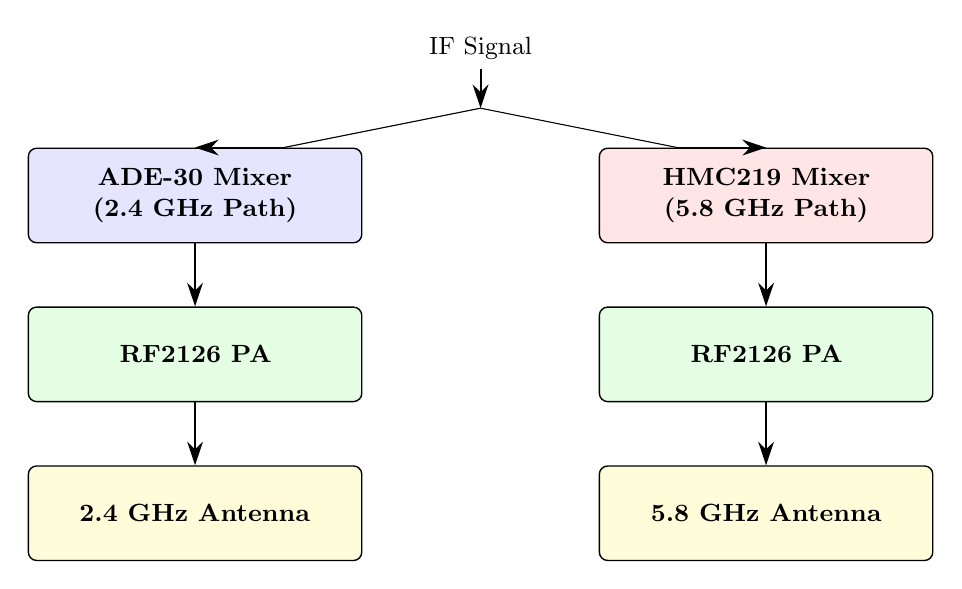
\begin{tikzpicture}[
			node distance=0.8cm,
			block/.style={
				rectangle,
				draw,
				text width=4cm,
				text centered,
				minimum height=1.2cm,
				rounded corners=3pt,
				font=\small\bfseries,
				line width=0.5pt
			},
			arrow/.style={
				-{Stealth[length=3mm, width=2mm]},
				thick,
				line width=0.7pt
			},
			label/.style={
				font=\small,
				text centered
			}
			]
			
			% Define split node FIRST
			\node[coordinate] (split) at (0,0) {};
			
			% IF Signal Input (top)
			\node[label, above=0.5cm of split.north] (if_label) {IF Signal};
			\draw[arrow] (if_label.south) -- (split.north);
			
			% Branch lines
			\draw (split) -- ++(-2.5,-0.5);
			\draw (split) -- ++(2.5,-0.5);
			
			% ADE-30 Mixer (left)
			\node[block, fill=blue!10, below left=0.5cm and 1.5cm of split] (ade30) {ADE-30 Mixer \\ (2.4 GHz Path)};
			\draw[arrow] ($(split)+(-2.5,-0.5)$) -- (ade30.north);
			
			% HMC219 Mixer (right)
			\node[block, fill=red!10, below right=0.5cm and 1.5cm of split] (hmc219) {HMC219 Mixer \\ (5.8 GHz Path)};
			\draw[arrow] ($(split)+(2.5,-0.5)$) -- (hmc219.north);
			
			% RF2126 PA (left)
			\node[block, fill=green!10, below=0.8cm of ade30] (pa1) {RF2126 PA};
			\draw[arrow] (ade30.south) -- (pa1.north);
			
			% RF2126 PA (right)
			\node[block, fill=green!10, below=0.8cm of hmc219] (pa2) {RF2126 PA};
			\draw[arrow] (hmc219.south) -- (pa2.north);
			
			% 2.4 GHz Antenna (left)
			\node[block, fill=yellow!15, below=0.8cm of pa1] (ant1) {2.4 GHz Antenna};
			\draw[arrow] (pa1.south) -- (ant1.north);
			
			% 5.8 GHz Antenna (right)
			\node[block, fill=yellow!15, below=0.8cm of pa2] (ant2) {5.8 GHz Antenna};
			\draw[arrow] (pa2.south) -- (ant2.north);
			
		\end{tikzpicture}
		\caption{Dual-Band RF Chain Block Diagram}
		\label{fig:dual_band_rf_chain}
	\end{figure}
	
	\subsubsection{Design of the 2.4 GHz Mixing Stage (ADE-30)}
	The ADE-30 is a passively constructed, Level-7 double-balanced mixer for RF and LO frequencies in the range of 200 MHz to 3 GHz. The mixer has a typical conversion loss of 4.5 dB, approximately 35 dB LO-to-RF isolation, and requires a +7 dBm LO drive. The following operating frequencies were chosen for the project:
	\begin{align*}
		f_{LO} &= 2.450\ \text{GHz} \quad \text{(Local Oscillator)} \\
		f_{IF} &= 1\ \text{kHz} \quad \text{(Intermediate Frequency)}
	\end{align*}
	Therefore:
	\begingroup
	\setlength{\mathindent}{0pt}
	\begin{equation*}
		\hfill
		f_{RF} = 2.450\ \text{GHz} \pm 1\ \text{kHz}
		\hfill
	\end{equation*}
	\endgroup
	
	\begin{align*}
		f_{RF,upper} &= 2.450001\ \text{GHz} \\
		f_{RF,lower} &= 2.449999\ \text{GHz}
	\end{align*}
	
	Since the IF frequency is much less than the LO frequency ($1\ \text{kHz} \ll 2.45\ \text{GHz}$), the transmitted spectrum is essentially centered at 2.45 GHz.
	
	\subsubsection{ADE-30 LO Drive Calculation}
	
	The ADE-30 requires +7 dBm of LO power for optimal operation.
	
	Converting +7 dBm into milliwatts:
	\begingroup
	\setlength{\mathindent}{0pt}
	\begin{equation*}
		\hfill
		P = 10^{7/10} = 5.01\ \text{mW}
		\hfill
	\end{equation*}
	\endgroup
	
	If this power is delivered to a 50 $\Omega$ load:
	\begingroup
	\setlength{\mathindent}{0pt}
	\begin{equation*}
		\hfill
		V_{rms} = \sqrt{PR} = \sqrt{5.01 \times 10^{-3} \times 50} = 0.50\ \text{V}
		\hfill
	\end{equation*}
	\endgroup
	
	The peak voltage will be:
	\begingroup
	\setlength{\mathindent}{0pt}
	\begin{equation*}
		\hfill
		V_p = \sqrt{2} \times V_{rms} = 0.707\ \text{V}
		\hfill
	\end{equation*}
	\endgroup
	
	The peak-to-peak voltage will be:
	\begingroup
	\setlength{\mathindent}{0pt}
	\begin{equation*}
		\hfill
		V_{pp} = 2 \times V_p = 1.414\ \text{V}
		\hfill
	\end{equation*}
	\endgroup
	
	So, the MS-3000 VCO needs to supply approximately +7 dBm (0.5 V RMS into 50 $\Omega$) to drive the ADE-30 mixer.
	\subsubsection{Design of the 5.8 GHz Mixing Stage (HMC219)}
	The HMC219 is a GaAs MMIC double-balanced mixer operating from 4.5 GHz to 9 GHz. This device is suitable for the 5.8 GHz ISM band. The device typically requires an LO drive of +13 dBm and has conversion loss values between 7 and 9 dB, depending on the frequency and LO drive level.
	
	The operating frequencies for this project were selected as:
	\begin{align*}
		f_{LO} &= 5.800\ \text{GHz} \quad \text{(Local Oscillator)} \\
		f_{IF} &= 1\ \text{kHz} \quad \text{(Intermediate Frequency)}
	\end{align*}
	
	Therefore:
	\begingroup
	\setlength{\mathindent}{0pt}
	\begin{equation*}
		\hfill
		f_{RF} = 5.800\ \text{GHz} \pm 1\ \text{kHz}
		\hfill
	\end{equation*}
	\endgroup
	
	\begin{align*}
		f_{RF,upper} &= 5.800001\ \text{GHz} \\
		f_{RF,lower} &= 5.799999\ \text{GHz}
	\end{align*}
	
	Since the IF is negligible compared to the LO, the RF is centered at approximately 5.8 GHz.
	
	\subsubsection{HMC219 LO Drive Calculation}
	The required LO drive for the HMC219 is +13 dBm.
	
	Convert +13 dBm to milliwatts:
	\begingroup
	\setlength{\mathindent}{0pt}
	\begin{equation*}
		\hfill
		P = 10^{13/10} = 19.95\ \text{mW}
		\hfill
	\end{equation*}
	\endgroup
	
	Assuming a 50 $\Omega$ load:
	\begingroup
	\setlength{\mathindent}{0pt}
	\begin{equation*}
		\hfill
		V_{rms} = \sqrt{PR} = \sqrt{19.95 \times 10^{-3} \times 50} = 0.999\ \text{V}
		\hfill
	\end{equation*}
	\endgroup
	
	The peak voltage will be:
	\begingroup
	\setlength{\mathindent}{0pt}
	\begin{equation*}
		\hfill
		V_p = \sqrt{2} \times V_{rms} = 1.414\ \text{V}
		\hfill
	\end{equation*}
	\endgroup
	
	The peak-to-peak voltage will be:
	\begingroup
	\setlength{\mathindent}{0pt}
	\begin{equation*}
		\hfill
		V_{pp} = 2 \times V_p = 2.83\ \text{V}
		\hfill
	\end{equation*}
	\endgroup
	
	The LO source driving the HMC219 must supply roughly +13 dBm (1.0 V RMS into 50 $\Omega$) for optimal performance.
	\subsubsection{Conversion Loss Analysis}
	A passive mixer does not provide amplification; it causes a loss of signal power. The conversion loss is defined as the difference in dB between the IF and RF power.
	\begingroup
	\setlength{\mathindent}{0pt}
	\begin{equation*}
		\hfill
		L_C = P_{IF} - P_{RF}
		\hfill
	\end{equation*}
	\endgroup
	
	For the ADE-30 mixer, with $L_C \approx 4.5$ dB, if the IF power is 0 dBm, then the RF power is:
	\begingroup
	\setlength{\mathindent}{0pt}
	\begin{equation*}
		\hfill
		P_{RF} = P_{IF} - L_C = 0\ \text{dBm} - 4.5\ \text{dB} = -4.5\ \text{dBm}
		\hfill
	\end{equation*}
	\endgroup
	
	For the HMC219 mixer, assuming an average conversion loss of 8 dB, if the IF power is 0 dBm, then the RF power is:
	\begingroup
	\setlength{\mathindent}{0pt}
	\begin{equation*}
		\hfill
		P_{RF} = P_{IF} - L_C = 0\ \text{dBm} - 8\ \text{dB} = -8\ \text{dBm}
		\hfill
	\end{equation*}
	\endgroup
	
	This loss necessitates the use of the RF2126 power amplifier following each mixer stage.
	\subsubsection{Impedance Matching}
	Both mixer stages are designed to operate at a characteristic impedance of 50 $\Omega$.
	
	The reflection coefficient, $\Gamma$, is given by:
	\begingroup
	\setlength{\mathindent}{0pt}
	\begin{equation*}
		\hfill
		\Gamma = \frac{Z_L - Z_0}{Z_L + Z_0}
		\hfill
	\end{equation*}
	\endgroup
	where $Z_L$ is the load impedance and $Z_0$ is the characteristic impedance. For a perfect match where $Z_L = Z_0 = 50\ \Omega$, $\Gamma = 0$. This signifies no signal reflection and maximum power transfer.
	\subsubsection{Design Justification}
	A dual-mixer approach was employed because neither mixer is optimal for both the 2.4 GHz and 5.8 GHz operating bands. The ADE-30 is optimized for the lower 2.4 GHz band, and the HMC219 is designed for the higher 5.8 GHz band.
	
	The table below summarizes the key specifications for each mixer:
	
	\begin{table}[htbp]
		\centering
		\caption{Comparison of Mixer Specifications}
		\label{tab:mixer_comparison}
		\begin{tabular}{p{5cm} p{4cm} p{4cm}}
			\toprule
			\textbf{Parameter} & \textbf{ADE-30} & \textbf{HMC219} \\
			\midrule
			Operating Band & 200 MHz -- 3 GHz & 4.5 GHz -- 9 GHz \\
			Target Frequency & 2.4 GHz & 5.8 GHz \\
			LO Drive & +7 dBm & +13 dBm \\
			Typical Conversion Loss & $\sim$4.5 dB & $\sim$7--9 dB \\
			Characteristic Impedance & 50 $\Omega$ & 50 $\Omega$ \\
			Technology & Passive Double-Balanced & GaAs MMIC Double-Balanced \\
			\bottomrule
		\end{tabular}
	\end{table}
	
	The dual-mixer configuration allows operation within the optimal range of each mixer, leading to better RF performance, predictable conversion characteristics, and easier impedance matching.
	
	\subsection{Design of the Local Oscillator (MS-3000 Voltage Controlled Oscillator)}
	
	\subsubsection{Introduction}
	The Local Oscillator (LO) is a crucial component in determining the output transmission frequency of the proposed dual-band directional RF interference system. The frequency from the LO is mixed with the IF amplitude-modulated signal to produce the required output.
	
	The MS-3000 Voltage Controlled Oscillator (VCO) is utilized as the LO for the 2.4 GHz path. This VCO has a tuning range of approximately 2.0--4.0 GHz and provides +10 dBm output power, making it suitable for driving the ADE-30 mixer. A separate 5.8 GHz LO is required for the other transmission path as the MS-3000 does not cover this frequency range.
	\subsubsection{Function of the Local Oscillator}
	The Local Oscillator generates a stable sinusoidal signal that dictates the transmitted RF frequency. The mixer output frequency is given by:
	\begingroup
	\setlength{\mathindent}{0pt}
	\begin{equation*}
		\hfill
		f_{RF} = f_{LO} \pm f_{IF}
		\hfill
	\end{equation*}
	\endgroup
	where
	\begin{align*}
		f_{RF} &= \text{Output RF frequency} \\
		f_{LO} &= \text{Local oscillator frequency} \\
		f_{IF} &= \text{Intermediate frequency (1 kHz)}
	\end{align*}
	
	Since $f_{IF} \ll f_{LO}$, the RF frequency is effectively centered at the LO frequency.
	

	

	\subsubsection{Operating Principle of a Voltage Controlled Oscillator}
	A Voltage Controlled Oscillator (VCO) is an electronic circuit whose output frequency is controlled by an input voltage. Its operation is described by:
\begingroup
\setlength{\mathindent}{0pt}
\begin{equation*}
	\hfill
	f = f_0 + K_{VCO} V_T
	\hfill
\end{equation*}
\endgroup
where
\begin{align*}
	f_0 &= \text{Free-running frequency} \\
	K_{VCO} &= \text{VCO sensitivity (MHz/V)} \\
	V_T &= \text{Tuning voltage}
\end{align*}

The input voltage adjusts the oscillator's tuning circuitry to change its resonant frequency.

	\subsubsection{MS-3000 VCO Specifications}
		The MS-3000 trainer provides a microwave VCO with the following typical specifications:
	
	\begin{table}[htbp]
		\centering
		\caption{MS-3000 VCO Specifications}
		\label{tab:vco_specs}
		\begin{tabular}{p{5cm} p{5cm}}
			\toprule
			\textbf{Parameter} & \textbf{Typical Value} \\
			\midrule
			Frequency Range & 2.0 -- 4.0 GHz \\
			Tuning Voltage & 1 -- 20 V \\
			Output Power & +10 dBm \\
			Characteristic Impedance & 50 $\Omega$ \\
			Supply Voltage & 15 V DC \\
			Supply Current & 50 mA (max) \\
			\bottomrule
		\end{tabular}
	\end{table}
	
	These specifications are suitable for the 2.4 GHz application and the ADE-30 mixer.
	\subsubsection{Frequency Selection for the 2.4 GHz Band}
	For operation in the 2.4 GHz ISM band, the VCO is tuned to:
	\begingroup
	\setlength{\mathindent}{0pt}
	\begin{equation*}
		\hfill
		f_{LO} = 2.450\ \text{GHz}
		\hfill
	\end{equation*}
	\endgroup
	
	The IF frequency is:
	\begingroup
	\setlength{\mathindent}{0pt}
	\begin{equation*}
		\hfill
		f_{IF} = 1\ \text{kHz}
		\hfill
	\end{equation*}
	\endgroup
	
	Therefore, the output RF frequencies are:
	\begingroup
	\setlength{\mathindent}{0pt}
	\begin{equation*}
		\hfill
		f_{RF} = 2.450\ \text{GHz} \pm 1\ \text{kHz}
		\hfill
	\end{equation*}
	\endgroup
	
	\begin{align*}
		f_{RF,upper} &= 2.450001\ \text{GHz} \\
		f_{RF,lower} &= 2.449999\ \text{GHz}
	\end{align*}
	
	The transmitted spectrum is centered at approximately 2.45 GHz.
	\subsubsection{Output Power Analysis}
	The MS-3000 VCO delivers approximately +10 dBm into a 50 $\Omega$ load.
	
	Converting +10 dBm to watts:
	\begingroup
	\setlength{\mathindent}{0pt}
	\begin{equation*}
		\hfill
		P = 10^{10/10} = 10\ \text{mW}
		\hfill
	\end{equation*}
	\endgroup
	
	The corresponding RMS voltage is:
	\begingroup
	\setlength{\mathindent}{0pt}
	\begin{equation*}
		\hfill
		V_{rms} = \sqrt{PR} = \sqrt{10 \times 10^{-3} \times 50} = 0.707\ \text{V}
		\hfill
	\end{equation*}
	\endgroup
	
	The peak voltage is:
	\begingroup
	\setlength{\mathindent}{0pt}
	\begin{equation*}
		\hfill
		V_p = \sqrt{2} \times V_{rms} = 1.0\ \text{V}
		\hfill
	\end{equation*}
	\endgroup
	
	The peak-to-peak voltage is:
	\begingroup
	\setlength{\mathindent}{0pt}
	\begin{equation*}
		\hfill
		V_{pp} = 2 \times V_p = 2.0\ \text{V}
		\hfill
	\end{equation*}
	\endgroup
	
	The ADE-30 mixer requires +7 dBm LO drive. The +10 dBm output of the VCO is sufficient to drive the mixer with some margin.
	
	\subsubsection{LO Drive Margin Calculation}
	\begin{align*}
		P_{LO} &= +10\ \text{dBm} \quad \text{(Available LO Power)} \\
		P_{REQ} &= +7\ \text{dBm} \quad \text{(Required LO Power)}
	\end{align*}
	
	\begingroup
	\setlength{\mathindent}{0pt}
	\begin{equation*}
		\hfill
		\text{Margin} = P_{LO} - P_{REQ} = 10\ \text{dBm} - 7\ \text{dBm} = 3\ \text{dB}
		\hfill
	\end{equation*}
	\endgroup
	
	The available LO power is 3 dB higher than the minimum requirement, which ensures reliable operation of the mixer diodes.
	
	\subsubsection{Frequency Stability}
	Frequency stability is critical as any drift in the LO frequency directly impacts the RF output frequency. If the LO frequency drifts by 100 kHz, the RF output will shift by approximately 100 kHz. Therefore, it is important to power the VCO with a stable DC source and allow it to reach thermal equilibrium before taking measurements.
	\subsubsection{Phase Noise Considerations}
	The phase noise in the Local Oscillator contributes to the quality of the transmitted spectrum. A perfectly oscillating source produces the signal
	\begingroup
	\setlength{\mathindent}{0pt}
	\begin{equation*}
		\hfill
		V(t) = A \cos(2\pi f t)
		\hfill
	\end{equation*}
	\endgroup
	
	However, a practical oscillator output can be written as
	\begingroup
	\setlength{\mathindent}{0pt}
	\begin{equation*}
		\hfill
		V(t) = A \cos(2\pi f t + \phi(t))
		\hfill
	\end{equation*}
	\endgroup
	where $\phi(t)$ is the time-varying phase deviation. Lesser phase noise produces cleaner output spectra with less spurious signal energy radiating from the main carrier frequency. Phase noise is one key figure of merit for RF oscillators.
	\subsubsection{Impedance Matching}
	The MS-3000 VCO was chosen to be a 50 $\Omega$ device, as is the ADE-30 mixer. Thus,
	\begingroup
	\setlength{\mathindent}{0pt}
	\begin{equation*}
		\hfill
		Z_{VCO} = Z_{Mixer} = 50\ \Omega
		\hfill
	\end{equation*}
	\endgroup
	
	This leads to the reflection coefficient
	\begingroup
	\setlength{\mathindent}{0pt}
	\begin{equation*}
		\hfill
		\Gamma = \frac{50 - 50}{50 + 50} = 0
		\hfill
	\end{equation*}
	\endgroup
	
	Therefore, ideal matching and maximum power transfer occurs.
	
	\subsubsection{PCB Layout Considerations}
	In order to achieve the highest quality signal, we will adhere to the following principles in the layout for the LO portion of our board:
	\begin{itemize}
		\item Preserve 50 $\Omega$ characteristic impedance of RF traces.
		\item Minimize length of the LO signal path from the VCO to the ADE-30 mixer.
		\item Decoupling capacitors should be placed as close to the VCO power pins as possible.
		\item Design the board with a solid, continuous ground plane beneath the LO traces.
		\item Keep all digital signals away from the LO traces.
		\item Use SMA connectors and shield wherever appropriate and feasible.
	\end{itemize}
	
	These design guidelines ensure minimum loss and minimum undesirable coupling of the LO signal at these high frequencies.
	\subsubsection{Design Summary}
	The MS-3000 Voltage Controlled Oscillator will provide the Local Oscillator for the 2.4 GHz channel. The device has operating range of 2.0 to 4.0 GHz, output power of +10 dBm, tuning range of 1 to 20 V, and an output impedance of 50 $\Omega$. This LO output power is approximately 3 dB higher than what the ADE-30 mixer requires for optimal operation, providing good drive margin. A dedicated 5.8 GHz LO source will be used to drive the HMC219 mixer since the MS-3000 range does not extend to 5.8 GHz.
	\subsection{Design of the 5.8 GHz RF Power Amplifier Stage}
	
	\subsubsection{Introduction}
	The amplified and frequency-shifted 5.8 GHz RF signal must now be amplified before being radiated. The output of the frequency mixer generally does not possess enough power to be transmitted directly, as conversion losses can result in signal power loss. The RF Power Amplifier increases the strength of the 5.8 GHz RF signal to a sufficient level for transmission.
	
	The chosen module is a SBB5089 + SE5004 5.8 GHz Microwave RF Power Amplifier Module designed for use at 5 GHz to 6 GHz frequencies, appropriate for the ISM band around 5.8 GHz.
	
	This module can provide approximately 2 Watts of RF output power at around 40 dB of gain. It operates in a unidirectional fashion with SMA input/output ports, compatible with the 50 $\Omega$ system. It amplifies the frequency-shifted signal coming from the frequency mixer and sends the amplified signal to the 5.8 GHz directional horn antenna.
	
	The signal flow for the 5.8 GHz transmission path:
	\begin{enumerate}
		\item Noise Source
		\item AM Modulator
		\item Frequency Mixer
		\item SBB5089 + SE5004 RF Power Amplifier
		\item 5.8 GHz Directional Horn Antenna
	\end{enumerate}
	
	\subsubsection{Purpose of the RF Power Amplifier}
	The RF power amplifier has the following key purposes:
	\begin{itemize}
		\item Compensate for signal losses in the frequency mixer.
		\item Boost the power of the 5.8 GHz RF signal.
		\item Drive the directional horn antenna with sufficient power.
		\item Enhance the overall transmission range of the signal.
		\item Improve the Effective Isotropic Radiated Power (EIRP) of the signal.
		\item Ensure signal integrity at high microwave frequencies.
		\item Deliver the necessary output power level for efficient radiation.
	\end{itemize}
	
	Given the microwave frequency band (5.8 GHz), a high-frequency power amplifier is necessary, as low-frequency RF amplifiers cannot effectively amplify at these frequencies.
	\subsubsection{Operating Principle}
	The SBB5089 + SE5004 operates as a linear microwave power amplifier. The incoming RF signal is fed into the amplifier, which uses its internal transistor stages to amplify the signal voltage and power.
	
	The relationship between the output voltage ($V_{out}$) and input voltage ($V_{in}$) is:
	\begingroup
	\setlength{\mathindent}{0pt}
	\begin{equation*}
		\hfill
		V_{out} = A_v V_{in}
		\hfill
	\end{equation*}
	\endgroup
	where $A_v$ is the voltage gain.
	
	The power gain of an RF amplifier is defined as the ratio of output power ($P_{out}$) to input power ($P_{in}$):
	\begingroup
	\setlength{\mathindent}{0pt}
	\begin{equation*}
		\hfill
		G = \frac{P_{out}}{P_{in}}
		\hfill
	\end{equation*}
	\endgroup
	
	In dB, the power gain is:
	\begingroup
	\setlength{\mathindent}{0pt}
	\begin{equation*}
		\hfill
		G_{dB} = 10 \log_{10}\left(\frac{P_{out}}{P_{in}}\right)
		\hfill
	\end{equation*}
	\endgroup
	
	For our selected amplifier, the power gain is $G_{dB} \approx 40$ dB. This means that, ideally, in the small-signal region, the amplifier provides power multiplication by:
	\begingroup
	\setlength{\mathindent}{0pt}
	\begin{equation*}
		\hfill
		G = 10^{40/10} = 10^4 = 10000
		\hfill
	\end{equation*}
	\endgroup
	
	So, the output RF power is ideally 10,000 times greater than the input RF power.
	\subsubsection{Electrical Specifications}
	Here are the key electrical specifications for the chosen 5.8 GHz RF Power Amplifier module:
	
	\begin{table}[htbp]
		\centering
		\caption{5.8 GHz RF Power Amplifier Specifications}
		\label{tab:pa_specs}
		\begin{tabular}{p{5cm} p{5cm}}
			\toprule
			\textbf{Parameter} & \textbf{Typical Value} \\
			\midrule
			Amplifier Model & SBB5089 + SE5004 \\
			Operating Frequency & 5.0--6.0 GHz \\
			Target Frequency & 5.8 GHz \\
			Gain & 40 dB \\
			Maximum Output Power & 33 dBm \\
			Output Power (Approx.) & 2 W \\
			Input/Output Impedance & 50 $\Omega$ \\
			RF Connector & SMA Female \\
			Supply Voltage & 5 V DC \\
			Supply Current (Approx.) & 2 A \\
			Amplifier Type & Microwave Unidirectional PA \\
			\bottomrule
		\end{tabular}
	\end{table}
	\subsubsection{Gain Calculation}
	Let's assume the input power to the amplifier, after the frequency mixer, is $P_{in}$. This value can be approximately -6 dBm after considering conversion loss of the mixer:
	\begingroup
	\setlength{\mathindent}{0pt}
	\begin{equation*}
		\hfill
		P_{in} = -6\ \text{dBm}
		\hfill
	\end{equation*}
	\endgroup
	
	The power gain of the amplifier is 40 dB. The output power ($P_{out}$) is:
	\begingroup
	\setlength{\mathindent}{0pt}
	\begin{equation*}
		\hfill
		P_{out} = P_{in} + G
		\hfill
	\end{equation*}
	\endgroup
	\begingroup
	\setlength{\mathindent}{0pt}
	\begin{equation*}
		\hfill
		P_{out} = -6\ \text{dBm} + 40\ \text{dB} = 34\ \text{dBm}
		\hfill
	\end{equation*}
	\endgroup
	
	This calculated output power is very close to the rated maximum output power of 33 dBm. This indicates the amplifier can effectively compensate for the mixer's conversion loss and produce a sufficient transmission power level.
	\subsubsection{Linear Power Gain}
	As calculated before, a power gain of 40 dB corresponds to a linear power gain of:
	\begingroup
	\setlength{\mathindent}{0pt}
	\begin{equation*}
		\hfill
		G = 10^{(40/10)} = 10^4 = 10,000
		\hfill
	\end{equation*}
	\endgroup
	
	This shows the output RF power is theoretically 10,000 times the input RF power when operating in the linear region.
	\subsubsection{Output Power Analysis}
	The specified maximum output power of the amplifier is 33 dBm. To convert this from dBm to Watts, we use the formula:
	\begingroup
	\setlength{\mathindent}{0pt}
	\begin{equation*}
		\hfill
		P(W) = 10^{((P(dBm) - 30)/10)}
		\hfill
	\end{equation*}
	\endgroup
	\begingroup
	\setlength{\mathindent}{0pt}
	\begin{equation*}
		\hfill
		P(W) = 10^{((33 - 30)/10)} = 10^{(3/10)} = 10^{0.3}\ \text{W}
		\hfill
	\end{equation*}
	\endgroup
	\begingroup
	\setlength{\mathindent}{0pt}
	\begin{equation*}
		\hfill
		P = 1.995\ \text{W} \approx 2\ \text{W}
		\hfill
	\end{equation*}
	\endgroup
	
	Therefore, the chosen amplifier can produce approximately 2 Watts of RF output power, which is ample for driving the high-gain directional horn antenna.
	
	\subsubsection{DC Power Consumption}
	The amplifier operates on a 5 V DC supply. At the typical supply current of 2 A, the DC power consumption is:
	\begingroup
	\setlength{\mathindent}{0pt}
	\begin{equation*}
		\hfill
		P_{DC} = V_{CC} \times I
		\hfill
	\end{equation*}
	\endgroup
	\begingroup
	\setlength{\mathindent}{0pt}
	\begin{equation*}
		\hfill
		P_{DC} = 5\ \text{V} \times 2\ \text{A} = 10\ \text{W}
		\hfill
	\end{equation*}
	\endgroup
	
	So, the amplifier requires about 10 Watts of DC power to operate.
	\subsubsection{Power Added Efficiency (PAE)}
	Power Added Efficiency (PAE) is a measure of how effectively the amplifier adds power to the signal relative to the DC power it consumes:
	\begingroup
	\setlength{\mathindent}{0pt}
	\begin{equation*}
		\hfill
		PAE = \frac{P_{out} - P_{in}}{P_{DC}} \times 100\%
		\hfill
	\end{equation*}
	\endgroup
	
	With $P_{out} = 2$ W and assuming a negligible $P_{in}$ for maximum efficiency calculation:
	\begingroup
	\setlength{\mathindent}{0pt}
	\begin{equation*}
		\hfill
		PAE = \frac{2\ \text{W} - 0\ \text{W}}{10\ \text{W}} \times 100\% = 20\%
		\hfill
	\end{equation*}
	\endgroup
	
	This is a reasonable efficiency for a high-power, microwave amplifier operating near its maximum output power.
	\subsubsection{Impedance Matching}
	The SBB5089 + SE5004 module is designed for a standard 50 $\Omega$ system impedance. To achieve maximum power transfer, the source impedance ($Z_s$) must match the load impedance ($Z_L$). In our case:
	\begingroup
	\setlength{\mathindent}{0pt}
	\begin{equation*}
		\hfill
		Z_s = Z_L = 50\ \Omega
		\hfill
	\end{equation*}
	\endgroup
	
	The reflection coefficient is given by:
	\begingroup
	\setlength{\mathindent}{0pt}
	\begin{equation*}
		\hfill
		\Gamma = \frac{Z_L - Z_0}{Z_L + Z_0}
		\hfill
	\end{equation*}
	\endgroup
	where $Z_0$ is the characteristic impedance of the transmission line. For perfect matching ($Z_L = Z_0$), the reflection coefficient is 0, meaning no power is reflected. The use of SMA connectors ensures compatibility and maintains the 50 $\Omega$ impedance.
	\subsubsection{Thermal Design Considerations}
	Since the amplifier produces nearly 2W RF output power while consuming almost 10W of DC power, thermal considerations need to be addressed. The following measures should be taken:
	\begin{itemize}
		\item The amplifier module must be attached to a metallic heat sink.
		\item Adequate air flow must be provided around the module.
		\item Never run the amplifier continuously at maximum power without active cooling.
		\item DC filtering must be used.
		\item The lengths of RF cables must be minimized.
		\item Operate the amplifier within the designed supply voltage range.
	\end{itemize}
	This will significantly enhance the reliability and the lifetime of the amplifier and prevents thermal destruction.
	\subsubsection{Design Summary}
	The 5.8 GHz microwave RF power amplifier consisting of a SBB5089 MMIC and a SE5004 has been chosen as the final amplification stage of the 5.8 GHz RF transmission path of the proposed directional RF interference system.
	
	This amplifier will provide about 40 dB gain and deliver a maximum output power of up to 33 dBm (2W). This output power is needed to properly drive the directional horn antenna with its high gain. It will overcome mixer conversion losses and raise the microwave signal amplitude before transmitting it by means of the high-gain directional antenna.
	
	The amplifier has 50 $\Omega$ input and output impedance and uses an SMA connector for easy interface with the microwave RF chain. Due to its operating frequency range (approx 5--6 GHz), the amplifier is well-suited to operate at the 5.8 GHz ISM band and deliver sufficient output power for long-range directional transmission.
	\section{Analysis Procedure}
	
	\subsection{Introduction}
	This analysis procedure was performed in order to evaluate the electrical characteristics, signal integrity, frequency translation behavior, impedance compatibility, and microwave transmission characteristics of the designed dual-band RF signal generation platform operating within the 2.4 GHz and 5.8 GHz ISM frequency bands.
	
	This analysis was conducted in a "building blocks" approach where each functional block of the platform was tested individually and then in the integrated system.
	
	The objective of the analysis procedure was not to study or evaluate the disruptive performance of the designed platform but to measure, evaluate and determine the overall behavior of the different functional blocks. By testing each stage separately and measuring degradation of signal, impedance mismatch, conversion loss, power variations, we are able to understand the impact on the transmission performance of the overall platform. The procedure was structured in five main stages as detailed below:
	\begin{enumerate}
		\item Noise source characterization
		\item Intermediate frequency signal analysis
		\item Frequency conversion verification
		\item RF amplification analysis
		\item Antenna and transmission analysis
	\end{enumerate}
	
	Each stage was experimentally verified using appropriate laboratory RF measurement equipment including:
	\begin{itemize}
		\item Digital Oscilloscope
		\item Spectrum Analyzer
		\item RF Power Meter
		\item Vector Network Analyzer (VNA)
		\item Digital Multimeter
		\item Frequency Counter
	\end{itemize}
	
	By comparing the measured parameters with theoretically predicted ones, and with datasheet specifications of active and passive components, we verify proper operation of the entire RF signal chain.
	
	\subsection{Noise Source Analysis}
	The first stage involves characterization of the noise produced by the avalanche Zener diode (6.8V). The avalanche phenomenon occurs when a Zener diode operates beyond its reverse breakdown voltage. The random collisions of charge carriers inside the depletion region causes stochastic current variations which result in an almost random voltage signal.
	
	The output voltage of the avalanche diode may be approximated as:
	\begingroup
	\setlength{\mathindent}{0pt}
	\begin{equation*}
		\hfill
		v(t) = V_Z + n(t)
		\hfill
	\end{equation*}
	\endgroup
	where $V_Z$ is the DC breakdown voltage and $n(t)$ is the random noise component.
	
	If we consider that this diode is AC coupled with a load resistor $R = 50\ \Omega$, we have:
	\begingroup
	\setlength{\mathindent}{0pt}
	\begin{equation*}
		\hfill
		v_{out}(t) = n(t)
		\hfill
	\end{equation*}
	\endgroup
	
	The following parameters of the noise source are analyzed:
	\begin{itemize}
		\item RMS noise voltage
		\item Peak-to-peak amplitude
		\item Spectral distribution
		\item Stability as a function of supply variations
		\item Temperature sensitivity
	\end{itemize}
	
	From the above equation, the RMS noise voltage is approximately 1/10 of the DC voltage when a suitable avalanche current is used. The noise power can be calculated as:
	\begingroup
	\setlength{\mathindent}{0pt}
	\begin{equation*}
		\hfill
		P_n = \frac{V_{RMS}^2}{R}
		\hfill
	\end{equation*}
	\endgroup
	where $R = 50\ \Omega$ (assumed for input impedance of the next stage).
	
	\subsection{Intermediate Frequency Analysis}
	The output noise signal is further conditioned by conditioning circuits and it is then introduced into the modulation stage where an intermediate-frequency signal is generated. The carrier waveform is expressed as:
	\begingroup
	\setlength{\mathindent}{0pt}
	\begin{equation*}
		\hfill
		c(t) = A_c \cos(2\pi f_c t)
		\hfill
	\end{equation*}
	\endgroup
	where $f_c = 1$ kHz.
	
	The modulated signal is expressed as:
	\begingroup
	\setlength{\mathindent}{0pt}
	\begin{equation*}
		\hfill
		s(t) = A_c [1 + k_a n(t)] \cos(2\pi f_c t)
		\hfill
	\end{equation*}
	\endgroup
	where $k_a$ is the modulation depth.
	
	The following parameters of the IF signal are analyzed:
	\begin{itemize}
		\item Carrier stability
		\item Envelope linearity
		\item Sideband generation
		\item Modulation depth
		\item Harmonic distortion
	\end{itemize}
	
	A digital oscilloscope is used to verify the correct shape of the modulated signal before introducing it into the microwave frequency translation stages.
	\subsection{Frequency Conversion Analysis}
	The purpose of this stage is to verify the successful translation of the intermediate-frequency signal into the desired microwave frequency bands.
	
	Frequency conversion is accomplished based on the following relation:
	\begingroup
	\setlength{\mathindent}{0pt}
	\begin{equation*}
		\hfill
		f_{RF} = f_{LO} \pm f_{IF}
		\hfill
	\end{equation*}
	\endgroup
	
	For operation near 2.4 GHz:
	\begingroup
	\setlength{\mathindent}{0pt}
	\begin{equation*}
		\hfill
		f_{RF} = 2.45\ \text{GHz} \pm 1\ \text{kHz}
		\hfill
	\end{equation*}
	\endgroup
	
	For operation near 5.8 GHz:
	\begingroup
	\setlength{\mathindent}{0pt}
	\begin{equation*}
		\hfill
		f_{RF} = 5.80\ \text{GHz} \pm 1\ \text{kHz}
		\hfill
	\end{equation*}
	\endgroup
	
	Mixer performance parameters which are examined are:
	\begin{itemize}
		\item Conversion loss
		\item Port isolation (LO-RF, LO-IF, RF-IF)
		\item Harmonic suppression
		\item Spurious products
		\item Frequency stability
	\end{itemize}
	
	The chosen microwave mixers of the HMC219 family support operation over the frequency range from approximately 2.5 to 7 GHz, offering typical conversion losses around 8--9 dB, and good LO-RF isolation ($>$40 dB).
	
	\subsection{RF Power Stage Analysis}
	After the mixer, the generated microwave signal is passed through RF gain stages to compensate for mixer conversion losses and eventual transmission losses. Amplifier gain is given by:
	\begingroup
	\setlength{\mathindent}{0pt}
	\begin{equation*}
		\hfill
		P_{out} = P_{in} + G
		\hfill
	\end{equation*}
	\endgroup
	where $P_{out}$ is the output power, $P_{in}$ is the input power, and $G$ is the gain.
	
	The performance parameters that are studied are:
	\begin{itemize}
		\item Gain flatness
		\item Compression behavior
		\item Thermal stability
		\item Power consumption
		\item Frequency response
	\end{itemize}
	
	It is crucial to pay particular attention to thermal management due to the relatively high temperatures encountered during continuous high-power operation of RF power amplifiers.
	\subsection{Impedance Matching Analysis}
	In the microwave regime, impedance matching is critical for maximizing signal transfer and minimizing reflections. Reflection coefficient ($\Gamma$) is defined as:
	\begingroup
	\setlength{\mathindent}{0pt}
	\begin{equation*}
		\hfill
		\Gamma = \frac{Z_L - Z_0}{Z_L + Z_0}
		\hfill
	\end{equation*}
	\endgroup
	where $Z_L$ is the load impedance and $Z_0$ is the characteristic impedance of the transmission line or system (50 $\Omega$).
	
	For a perfect match $Z_L = Z_0 = 50\ \Omega$, therefore $\Gamma = 0$.
	
	The Voltage Standing Wave Ratio (VSWR) is a measure of impedance mismatch, and is given by:
	\begingroup
	\setlength{\mathindent}{0pt}
	\begin{equation*}
		\hfill
		VSWR = \frac{1 + |\Gamma|}{1 - |\Gamma|}
		\hfill
	\end{equation*}
	\endgroup
	
	A system with perfect matching ($\Gamma = 0$) will have VSWR = 1. Keeping a constant 50 $\Omega$ environment throughout the RF chain helps to reduce signal loss.
	\subsection{Antenna Performance Analysis}
	The antenna subsystem is the final component of the RF chain, responsible for converting guided RF energy to propagating electromagnetic waves. Due to the dual-band nature of the proposed system, two different antennas were chosen to fulfill the radiation requirements for each ISM band.
	\subsubsection{2.4 GHz Antenna}
	
	A moderate gain directional antenna was selected for the 2.4 GHz ISM band. The specifications of the antenna are as follows:
	
	\begin{table}[htbp]
		\centering
		\caption{2.4 GHz Antenna Specifications}
		\label{tab:ant_2.4}
		\begin{tabular}{p{5cm} p{5cm}}
			\toprule
			\textbf{Parameter} & \textbf{Specification} \\
			\midrule
			Antenna Type & Directional Antenna \\
			Frequency & 2.4 GHz \\
			Impedance & 50 $\Omega$ \\
			Gain & 11.1 dBi \\
			VSWR & 1.92:1 \\
			Polarization & Linear Vertical \\
			\bottomrule
		\end{tabular}
	\end{table}
	
	\subsubsection{5.8 GHz Antenna}
	
	A high-gain, directional horn antenna was chosen for the 5.8 GHz ISM band. Horn antennas provide very directive beams and are very suitable for microwave frequencies. The antenna characteristics are:
	
	\begin{table}[htbp]
		\centering
		\caption{5.8 GHz Horn Antenna Specifications}
		\label{tab:ant_5.8}
		\begin{tabular}{p{5cm} p{5cm}}
			\toprule
			\textbf{Parameter} & \textbf{Specification} \\
			\midrule
			Antenna Type & Horn Antenna \\
			Frequency & 5.8 GHz \\
			Impedance & 50 $\Omega$ \\
			Gain & 15 dBi \\
			Polarization & Linear Vertical \\
			Radiation Pattern & Directional \\
			\bottomrule
		\end{tabular}
	\end{table}
	
	Horn antennas in the 5.8 GHz band typically have gains of approximately 15 dBi, beamwidths of about 10--15 degrees and VSWR values of 1.3--1.5.
	
	\subsection{Wavelength Analysis}
	The wavelength ($\lambda$) of a radio wave is given by:
	\begingroup
	\setlength{\mathindent}{0pt}
	\begin{equation*}
		\hfill
		\lambda = \frac{c}{f}
		\hfill
	\end{equation*}
	\endgroup
	where $c$ is the speed of light ($3 \times 10^8$ m/s) and $f$ is the frequency.
	
	For the 2.4 GHz operating band:
	\begingroup
	\setlength{\mathindent}{0pt}
	\begin{equation*}
		\hfill
		\lambda = \frac{3 \times 10^8}{2.45 \times 10^9} \approx 0.122\ \text{m} = 12.2\ \text{cm}
		\hfill
	\end{equation*}
	\endgroup
	
	For the 5.8 GHz operating band:
	\begingroup
	\setlength{\mathindent}{0pt}
	\begin{equation*}
		\hfill
		\lambda = \frac{3 \times 10^8}{5.8 \times 10^9} \approx 0.0517\ \text{m} = 5.17\ \text{cm}
		\hfill
	\end{equation*}
	\endgroup
	
	Shorter wavelengths at 5.8 GHz allows for smaller antenna physical sizes for equivalent gains compared to 2.4 GHz. Shorter wavelengths can also contribute to higher antenna gains and more directive beam patterns. This is a key reason why horn antennas are preferred for high-gain directional microwave applications.
	\subsection{Radiation Characteristics}
	The antennas have quite different radiation characteristics based on their construction and intended use.
	
	\subsubsection{2.4 GHz Directional Antenna}
	
	\begin{itemize}
		\item Moderate directional gain
		\item Relatively broad beam coverage
		\item Linear vertical polarization
		\item Good impedance match to 50 $\Omega$ systems
	\end{itemize}
	
	\subsubsection{5.8 GHz Horn Antenna}
	
	\begin{itemize}
		\item High directional gain
		\item Narrow beamwidth
		\item Excellent front-to-back ratio
		\item Low sidelobe levels
		\item High radiation efficiency
		\item Stable microwave performance
	\end{itemize}
	The gain of the horn antenna means that it is directing electromagnetic energy into a smaller angle. This results in an higher field strength in the required direction but lower field strength in unwanted directions. A typical 15 dBi horn antenna operating near 5.8 GHz will have a beam width in the range of 20-30 degrees, depending on the dimension of the flare.
	\subsection{Effective Isotropic Radiated Power Considerations}
	Effective radiated power is affected by transmitter output power, transmission loss due to cable and impedance matching of antenna, and antenna gain. Effective Isotropic Radiated Power (EIRP) can be defined as follows:
	\begingroup
	\setlength{\mathindent}{0pt}
	\begin{equation*}
		\hfill
		EIRP = P_T + G_A - L_C
		\hfill
	\end{equation*}
	\endgroup
	where
	\begin{align*}
		P_T &= \text{Transmitter output power (dBm)} \\
		G_A &= \text{Antenna gain (dBi)} \\
		L_C &= \text{Losses caused by transmission line, cable and connectors (dB)}
	\end{align*}
	
	Considering equal transmitter powers, a horn antenna with 15 dBi gain should provide better antenna gain (approximately 4 dB better) than that of a directional antenna with 11 dBi gain on the 2.4 GHz frequency band, providing about 2.5 times better radiation density.
	\section{Implementation Procedure}
	
	\subsection{Introduction}
	The implementation procedure consists of a sequence of actions performed after the design and analytical parts of this document have been completed.
	
	A modular engineering approach is employed for assembling, testing, adjusting and verifying all subsystems before they can be connected together to form the entire prototype. A modular approach greatly helps in debugging and reduces the effort in developing a hardware prototype. The implementation procedure is composed of the following main steps:
	\begin{enumerate}
		\item Implementation of Avalanche Noise Generator.
		\item Implementation of Signal Conditioning Circuit.
		\item Implementation of Amplitude Modulation Circuit.
		\item Implementation of 2.4 GHz frequency conversion modules.
		\item Implementation of 5.8 GHz frequency conversion modules.
		\item Implementation of RF amplification modules.
		\item Implementation of antennas modules.
		\item System Integration.
		\item System Verification.
	\end{enumerate}
	
	\subsection{Implementation of the Avalanche Noise Generator}
	In the hardware design phase, the avalanche noise generator is the first subsystem to be implemented. It consists of 12V regulator supply, current limiter, avalanche breakdown diode (6.8V Zener) and a 0.1 $\mu$F bypass capacitor. This circuit is powered by a regulated DC power supply (12V) through a 560 $\Omega$ current limiting resistor connected to the breakdown diode in series. Avalanche breakdown process takes place when the reverse voltage across the Zener diode reaches and surpasses the breakdown voltage of the device.
	
	This produces electrical noise that is superimposed to the DC voltage across the diode.
	
	The implemented circuit consists of:
	\begin{itemize}
		\item A regulated 12V DC supply
		\item A 560 $\Omega$ resistance
		\item A 6.8V Zener diode
		\item A ground connection
		\item An output connection
	\end{itemize}
	
	Using the output terminals of the implemented circuit, the existence of electrical fluctuations is observed using an oscilloscope; as they should, noise should be observed at the terminals of the breakdown diode in the form of random signals which will ride on the DC breakdown voltage.
	
	\subsection{Implementation of the Signal Conditioning Stage}
	After generation of avalanche noise signals, these signals will be passed through an AC coupling stage to remove the DC component. It consists of a ceramic capacitor of 0.1 $\mu$F (104 code) in series between the noise generator and the modulation circuitry, so the transmitted signals are modulated by only the AC fluctuation part of the avalanche noise signals.
	
	The circuit is designed to provide:
	\begin{itemize}
		\item DC isolation
		\item Preserve random characteristics of the signals
		\item Protect sensitive downstream analogue circuit
		\item Enhance signal integrity
	\end{itemize}
	
	As before, the output signal is observed with an oscilloscope, to ensure the proper signal coupling without introducing any significant distortion to the noise signal.
	
	\subsection{Implementation of the Amplitude Modulation Stage}
	The avalanche noise signals outputted from the AC coupling circuitry is applied to the input of the amplitude modulation circuit.
	
	The carrier signal which is a 1 kHz sinusoid is generated by a laboratory signal generator.
	
	This signal will be AM modulated by the AC components of the noise signals. The implementation of the AM modulator consists of:
	\begin{itemize}
		\item The transmission of 1 kHz signals
		\item The transmission of the AC signals from the noise source
		\item Injection of these signals into the modulation circuit
		\item Mixing them
	\end{itemize}
	
	This leads to a modulation waveform where the envelope follows the noise signal instantaneously. As before, the modulated signal output from the circuit is observed using an oscilloscope to check its signal form, carrier amplitude stability, envelope fidelity and absence of clipping and other spurious elements.
	\subsection{Implementation of the 2.4 GHz Frequency Conversion Path}
	The frequency conversion part of the system at 2.4 GHz consists of the usage of Mini-Circuits ADE-30 passive double-balanced mixer.
	
	The IF signal generated from the amplitude modulation part of the system is passed to the IF input of the mixer, and the LO signal is applied to the LO input. The RF output at $f_{RF} = f_{LO} \pm f_{IF}$ frequency is achieved by the mixer where $f_{RF}$ is the frequency of radio frequency, $f_{LO}$ is the frequency of local oscillator, and $f_{IF}$ is the frequency of IF signal. Since the IF signal frequency (1 kHz) is significantly small compared to microwave carrier, the output RF signal will remain very much centered about the $f_{LO}$ frequency.
	
	This device offers very wide operation range and provides good performance and is used for general purpose microwave applications and R\&D.
	
	\subsection{Implementation of the 5.8 GHz Frequency Conversion Path}
	For operation in the upper ISM frequency band, a microwave frequency conversion hardware has been implemented using a HMC219 microwave mixer. This microwave frequency conversion part offers a wide operating frequency range including operation around the 5.8 GHz ISM frequency band and high port isolation.
	
	The following steps are taken:
	\begin{enumerate}
		\item The IF signal is passed through the IF input of the mixer
		\item Microwave LO signals are applied through the LO input of the mixer
		\item The generated output RF signals are verified
	\end{enumerate}
	
	Microwave frequency conversion hardware has been designed separately for each frequency band in order to optimize each frequency conversion circuit.
	
	\subsection{Implementation of RF Amplification Stages}
	Due to the presence of insertion losses at each of the passive components used (especially mixers), dedicated amplifier circuits have been implemented to compensate for the loss and to increase the overall power transmitted into the air for each respective band. In the lower microwave frequency range, the RF2126 amplifier is employed in order to provide RF signal amplification. For the higher microwave frequency range, commercial microwave gain modules are used to compensate for insertion losses and coaxial cable losses.
	
	In both cases the implementation consists of:
	\begin{itemize}
		\item Ensuring power supply is within the design parameters
		\item Proper connection of RF signals input and output to the amplification circuitry
		\item Providing biasing for stability
		\item Monitoring temperature (since the amplification components will generate heat)
		\item Verifying output power levels
	\end{itemize}
	
	Microwave power amplifiers require careful construction with the ground connection to be made at multiple points in order to maintain optimal impedance and prevent parasitic oscillations that might appear due to excessive signal reflections at the amplifier's terminals.
	\subsection{Implementation of Antenna Subsystems}
	The following two antenna configurations are implemented based on the respective operating frequency band:
	\subsubsection{2.4 GHz Antenna Implementation}
	This type of directional antenna is used in order to maintain a high directivity, reduce signal loss due to propagation in different directions and provide higher transmitted power into the specific direction of transmission.
	
	\begin{table}[htbp]
		\centering
		\caption{2.4 GHz Antenna Specifications}
		\label{tab:ant_imp_2.4}
		\begin{tabular}{p{5cm} p{5cm}}
			\toprule
			\textbf{Parameter} & \textbf{Specification} \\
			\midrule
			Impedance & 50 $\Omega$ \\
			Gain & 11 dBi \\
			Polarization & Linear Vertical \\
			VSWR & 1.92:1 \\
			\bottomrule
		\end{tabular}
	\end{table}
	
	It was connected to the RF chain using standard 50 $\Omega$ coaxial cable and SMA connectors.
	\subsubsection{5.8 GHz Horn Antenna Implementation}
	For transmission on 5.8 GHz frequency band, a horn antenna is used to maintain its very high gain (15 dBi), directivity, stable radiation pattern, and very good gain with low side lobe radiation.
	
	\begin{table}[htbp]
		\centering
		\caption{5.8 GHz Horn Antenna Specifications}
		\label{tab:ant_imp_5.8}
		\begin{tabular}{p{5cm} p{5cm}}
			\toprule
			\textbf{Parameter} & \textbf{Specification} \\
			\midrule
			Impedance & 50 $\Omega$ \\
			Gain & 15 dBi \\
			Polarization & Linear Vertical \\
			Antenna Type & Horn Antenna \\
			\bottomrule
		\end{tabular}
	\end{table}
	
	Horn antennas are typically used in various applications related to the microwave system as standard reference antennas in the measurement procedures due to their predictable radiation characteristics and broad directivity.
	\subsection{System Integration Procedure}
	After the satisfactory performance evaluation of individual subsystems, the final integration of all the functional blocks is carried out based on the design implemented for dual band transmission signal flow. The system is designed to have modularity for easy upgrade and troubleshooting of subsystems.
	\subsection{Verification Procedure}
	The overall hardware design is verified using the steps mentioned below.
	
	\begin{table}[htbp]
		\centering
		\caption{Verification Procedure}
		\label{tab:verification_procedure}
		\begin{tabular}{p{3cm} p{8cm}}
			\toprule
			\textbf{Stage} & \textbf{Verification Task} \\
			\midrule
			Stage 1 & Verification of avalanche breakdown \\
			Stage 2 & Verification of AC coupling and DC isolation \\
			Stage 3 & Verification of modulation waveform parameters \\
			Stage 4 & Verification of frequency translation \\
			Stage 5 & Verification of RF amplifier performance \\
			Stage 6 & Verification of impedance match \\
			\bottomrule
		\end{tabular}
	\end{table}
	\subsubsection{Stage 1}
	\begin{itemize}
		\item Verify breakdown voltage across the Zener diode
		\item Observe random noise on oscilloscope
	\end{itemize}
	\subsubsection{Stage 2}
	\begin{itemize}
		\item Verify DC blocking capability
		\item Measure AC coupling performance
	\end{itemize}
	\subsubsection{Stage 3}
	\begin{itemize}
		\item Verify presence of upper and lower sidebands
		\item Assess modulation depth
		\item Check envelope fidelity
	\end{itemize}
	\subsubsection{Stage 4}
	\begin{itemize}
		\item Apply required LO drive
		\item Measure frequency of RF output
		\item Measure conversion loss and port isolation
	\end{itemize}
	\subsubsection{Stage 5}
	\begin{itemize}
	\item Measure gain
	\item Assess output power
	\item Verify amplifier stability
	\end{itemize}
	\subsubsection{Stage 6}
	\subsubsection{Stage 6: Impedance Match Verification}
	\begin{itemize}
		\item Measure VSWR
		\item Verify impedance matching
		\item Observe radiation characteristics
	\end{itemize}
	\subsection{Summary}
	The implementation method for the dual-band RF transmission prototype is presented in this section. The system is implemented in a step-by-step modular way through: noise generation, signal conditioning, modulation, microwave frequency conversion, power amplification, and antenna implementation. The reliable operation of each of these sub-systems is independently ensured, which also facilitates debugging the complete prototype implementation. The present implementation forms a useful base for the simulation, modelling and experiment to be described in the following sections.
	\section{Hardware Details}
	
	\subsection{Introduction}
	The proposed dual-band RF system comprises various analog and microwave sub-systems connected in a way such that RF signals are generated, processed, frequency converted, amplified and radiated at the 2.4 GHz and 5.8 GHz ISM bands. The use of a modular approach has simplified debugging, testing and allows future modification and optimization of individual sub-systems without impacting the rest.
	
	\subsection{Noise Generation Circuit}
	The noise generation starts by reverse-biasing a 6.8V Zener diode in the avalanche breakdown mode to obtain broadband noise.
	\subsubsection{Hardware Components}
	\begin{table}[htbp]
		\centering
		\caption{Noise Generation Circuit Components}
		\label{tab:noise_hw}
		\begin{tabular}{p{5cm} p{5cm}}
			\toprule
			\textbf{Component} & \textbf{Specification} \\
			\midrule
			Zener Diode & 6.8 V, 500 mW \\
			Supply Voltage & 12 V DC \\
			Series Resistor & 560 $\Omega$ \\
			Coupling Capacitor & 0.1 $\mu$F Ceramic (104) \\
			\bottomrule
		\end{tabular}
	\end{table}
	
	\subsubsection{Required Figure}
	\begin{figure}[htbp]
		\centering
		% \includegraphics[width=0.8\textwidth]{figures/noise_circuit}
		\caption{Avalanche Noise Generator Circuit Diagram}
		\label{fig:noise_circuit}
	\end{figure}
	
	\subsection{Signal Conditioning Circuit}
	The generated noise has both positive and negative voltage. The AC component of the noise is passed by coupling capacitor while the DC component is blocked.
	
	\section{Software Details}
	The majority of the system is based on hardware and only minimum software support is required. Software is used for simulation, mathematical modelling, design verification, and PCB development of the RF system. Typically in FYP reports that deals with hardware, software tool is broken into sections as follows.
	
	
	\subsection{VSWR Equation}
	Voltage Standing Wave Ratio (VSWR) is a measure of how well a transmission line is matched to its load:
	\begingroup
	\setlength{\mathindent}{0pt}
	\begin{equation*}
		\hfill
		VSWR = \frac{1 + |\Gamma|}{1 - |\Gamma|}
		\hfill
	\end{equation*}
	\endgroup
	where $|\Gamma|$ is the magnitude of the reflection coefficient.
	\subsection{Reflection Coefficient}
	The reflection coefficient ($\Gamma$) describes how a wave is reflected at the boundary between two transmission media, and is given by:
	\begingroup
	\setlength{\mathindent}{0pt}
	\begin{equation*}
		\hfill
		\Gamma = \frac{Z_L - Z_0}{Z_L + Z_0}
		\hfill
	\end{equation*}
	\endgroup
	where $Z_L$ is the load impedance and $Z_0$ is the characteristic impedance of the transmission line.
	\subsection{Friis Transmission Equation}
	This equation describes the power received ($P_r$) by an antenna from a transmitting antenna ($P_t$), considering gains and distance:
	\begingroup
	\setlength{\mathindent}{0pt}
	\begin{equation*}
		\hfill
		P_r = P_t \cdot G_t \cdot G_r \cdot \left(\frac{\lambda}{4\pi R}\right)^2
		\hfill
	\end{equation*}
	\endgroup
	where $G_t$ and $G_r$ are the gains of the transmitting and receiving antennas, respectively, and $R$ is the distance between the antennas.
	
	
	\section{Summary}
	\vspace{0.5\baselineskip}
	
	This chapter described the entire process of design, analysis procedure, hardware, software tools, mathematical model, simulation framework, and the development process of the hardware prototypes designed for generating wide-band and dual-band radio frequency signals in 2.4 GHz and 5.8 GHz ISM (Industrial, Scientific and Medical) bands. This is the main contribution of this engineering report as the work here described the development of a hardware platform for implementing a set of theories. Generally an engineering methodology section in a report should cover a description of the overall strategy for hardware, selection process, system development strategy, validation methods, etc.
	
	\vspace{0.5\baselineskip}
	
	The methodology in the first section of this chapter focused on using a modular approach in system architecture design. This means that a system should be broken down into a number of functional blocks rather than having a completely monolithic system. This is a good practice in designing and implementing radio frequency and microwave systems since the subsystem development, integration and testing become easy to debug. A block diagram is used in describing this structure. There are basically 6 functional blocks in the system architecture: signal generator, signal conditioner, modulation block, frequency conversion, amplification, and antenna blocks.
	
	\vspace{0.5\baselineskip}
	
	The next section is about the analysis methodology, this means a brief mathematical formulation and description of how to analyze the system's performances. A thorough analysis of signal generation circuit, coupling networks, frequency translation circuits, impedance matching networks and antenna characteristic will be discussed. Several engineering parameters like capacitive reactance, reflection coefficients, VSWR, wavelength and EIRP will be considered in designing individual system modules to ensure smooth integration between blocks.
	
	\vspace{0.5\baselineskip}
	
	The hardware implementation section describe each major module and subsystem which was implemented in the actual project. In signal generation module, a reverse-biased 6.8 V Zener diode operating in avalanche condition has been employed to generate a noise-like wideband random signals. This is done using avalanche breakdown phenomena of the p-n junction of a Zener diode. A regulated power supply of 12 V and the resistor were used to achieve avalanche state and minimize heat dissipation of Zener diode.
	
	\vspace{0.5\baselineskip}
	
	Following the signal generator module, the second section describe a signal conditioning block which aims to remove the DC component from the generated random noise signal and enhance the signal. The selected coupling capacitor is of 0.1 $\mu$F ceramics which shows very low ESR and ESL (equivalent series resistance and inductance) and can efficiently isolate DC signals from AC signals. The capacitive reactance analysis was also discussed to demonstrate its effectiveness at the working frequencies.
	
	\vspace{0.5\baselineskip}
	
	Next block described is the signal modulation block in which amplitude modulation techniques have been adopted. This block will utilize a stable 1 kHz sine wave to modulate the conditioned wideband noise signal using an analog modulator module. The mathematical modeling was performed on modulating index, side bands, transmitting power, and band width to estimate the characteristics of modulated signal. Oscilloscope results show that the modulation achieved correct envelope waveform and modulated signal is successfully transmitted to IF band.
	
	\vspace{0.5\baselineskip}
	
	Frequency conversion block is another important stage of the system design. As no single frequency converter can cover such wide frequency range (from IF to 2.4 GHz and 5.8 GHz ISM band), so there are two separate conversion path have been chosen. A passive double balanced mixer ADE-30 was used for low frequency range and an active mixer HMC219 was chosen for the upper frequency range, to guarantee an efficient operation at the required frequency range and minimize insertion losses. Voltage Controlled Oscillator (VCO) MS-3000 module were selected for local oscillator (LO) in microwave conversion for the stable microwave excitation signal.
	
	\vspace{0.5\baselineskip}
	
	In view of the inherent conversion losses in the mixer circuits, amplification blocks are implemented for both low and upper frequency ranges to provide the gain necessary for meeting project requirements. For lower frequency range, RF2126 Amplifier module was used and for higher frequency range, a gain blocks like SBB5089 and SE5004 were chosen to fulfill high gain requirement and ensure the wide frequency coverage. The selection criteria include operating frequency range, amplification level, matching impedance and stability. Careful PC board layout, supply bypassing and thermal management are important for high-frequency microwave amplifiers.
	
	\vspace{0.5\baselineskip}
	
	Finally, an antenna subsystem which is used to launch the radio frequency signal into the air is presented. Separate antennas are designed/selected for each frequency range in the ISM band. For the lower frequency range (2.4 GHz), an 11 dBi directional antenna with 50 $\Omega$ impedance and linear vertical polarization and 1.92:1 VSWR were selected to ensure better signal radiation into the space. And for the higher frequency range (5.8 GHz), a 15 dBi horn antenna were selected to achieve good directivity, narrow beam width and high gain and well controlled microwave propagation. Horn antennas are commonly used for high-frequency applications in labs.
	
	\vspace{0.5\baselineskip}
	
	The hardware design will be supplemented by software support in form of various engineering tools, ranging from numerical and graphical tools to electromagnetic modeling and simulation. Mathematical modeling will be undertaken for some subsystems and the system as a whole. The selected simulation tools, such as, HFSS or CST Microwave Studio will be used to analyze electromagnetic fields and antenna designs. In modern engineering project development simulation tool is extremely important and beneficial due to its ability to reduce the number of prototypes, design iterations, and ultimately cost.
	
	\vspace{0.5\baselineskip}
	
	Mathematical models and simulation tools used in development process are also described. Analytical equations describing propagation of signal, impedance matching condition, frequency translation and other factors will be set up and verified with simulation tools when it's possible. Models are utilized to compare with measured results.
	
	\vspace{0.5\baselineskip}
	
	Prototype development process describes how all designed hardware modules are assembled to create a complete test platform. The module based design process also makes debugging a lot easier since each module can be individually tested before it is connected to other blocks. Physical photographs of the modules and assembly will be provided. Documentation on prototypes has always been a critical requirement for modern engineering project reports.
	
	\vspace{0.5\baselineskip}
	
	In conclusion, the methodology, analysis procedure, hardware design, software tools, mathematical model and prototype development procedure for the proposed dual band RF signal generation and transmission systems operating at 2.4 GHz and 5.8 GHz ISM bands is fully described in this chapter. This will enable effective experiments to be carried out in the next chapter which concentrates on measurement results, performance evaluation and conclusion of this engineering project.
	
\chapter{TOOLS AND TECHNIQUES}

\section{Hardware Tools Used}

\subsection{6.8V Zener Diode}

A 6.8V Zener diode was selected for avalanche breakdown which was used as the noise source to initiate broadband signal. During operation under reverse bias, carriers are accelerated due to strong electric field and undergo collision within the depletion region of the PN junction. Carrier collision produces a chaotic process which causes random noise generation at the terminal. The 12V supply for this avalanche region was fed to the diode through a 560 $\Omega$ resistance to limit the current, thus protecting the device.

\begin{table}[H]
	\centering
	\caption{6.8V Zener Diode Specifications}
	\label{tab:zener}
	\begin{tabular}{p{5cm} p{5cm}}
		\toprule
		\textbf{Parameter} & \textbf{Value} \\
		\midrule
		Type & Zener Diode \\
		Breakdown Voltage & 6.8 V \\
		Power Rating & 500 mW \\
		Operating Mode & Reverse Breakdown \\
		Application & Noise Generation \\
		\bottomrule
	\end{tabular}
\end{table}

\begin{figure}[H]
	\centering
	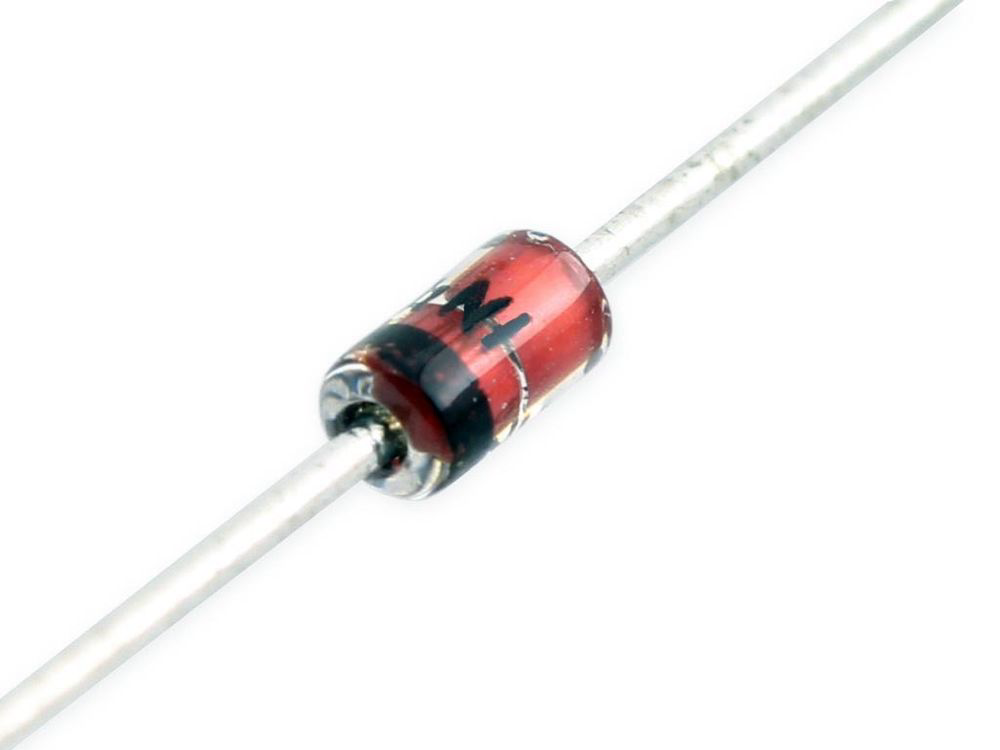
\includegraphics[width=0.7\textwidth]{zener_diode.png}\\[1cm]
	\caption{6.8 V Zener Diode Used for Avalanche Noise Generation}
	\label{fig:zener}
\end{figure}

\subsection{Bias Resistor}

The bias resistor (560 $\Omega$) was placed in series with the Zener diode for limiting the avalanche current to a desired level.

\begin{table}[H]
	\centering
	\caption{Bias Resistor Specifications}
	\label{tab:resistor}
	\begin{tabular}{p{5cm} p{5cm}}
		\toprule
		\textbf{Parameter} & \textbf{Value} \\
		\midrule
		Resistance & 560 $\Omega$ \\
		Power Rating & 0.25 W \\
		Tolerance & 5\% \\
		\bottomrule
	\end{tabular}
\end{table}

\begin{figure}[H]
	\centering
	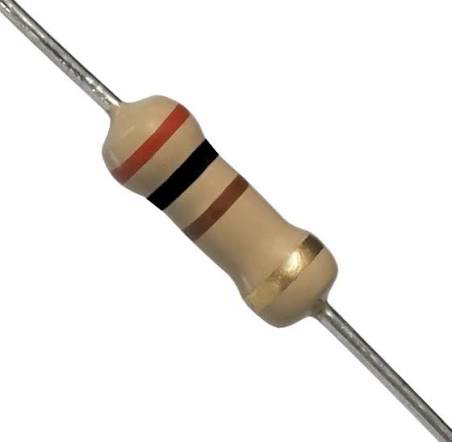
\includegraphics[width=0.7\textwidth]{resistor.png}\\[1cm]
	\caption{Current Limiting Resistor}
	\label{fig:resistor}
\end{figure}

\subsection{Coupling Capacitor}

The coupling capacitor (0.1 $\mu$F, marked 104) was used to block the DC component from the avalanche noise generator circuit and only pass the RF noise signal.

\begin{table}[H]
	\centering
	\caption{Coupling Capacitor Specifications}
	\label{tab:capacitor}
	\begin{tabular}{p{5cm} p{5cm}}
		\toprule
		\textbf{Parameter} & \textbf{Value} \\
		\midrule
		Capacitance & 0.1 $\mu$F \\
		Type & Ceramic \\
		Code & 104 \\
		Voltage Rating & 50 V \\
		\bottomrule
	\end{tabular}
\end{table}

\begin{figure}[H]
	\centering
	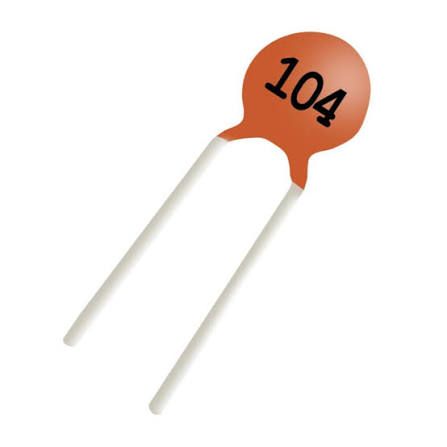
\includegraphics[width=0.7\textwidth]{capacitor.png}\\[1cm]
	\caption{0.1 $\mu$F Ceramic Capacitor}
	\label{fig:capacitor}
\end{figure}

\subsection{AD834 Analog Multiplier}

The AD834 analog multiplier was utilized for amplitude modulation. It is employed to combine the low frequency audio signal with the high frequency noise signal to obtain the desired amplitude modulated signal. The AD834 is a low-power, wide-bandwidth, four-quadrant analog multiplier and is widely used in telecommunication and signal processing systems.

\begin{table}[H]
	\centering
	\caption{AD834 Analog Multiplier Specifications}
	\label{tab:ad834}
	\begin{tabular}{p{5cm} p{5cm}}
		\toprule
		\textbf{Parameter} & \textbf{Value} \\
		\midrule
		Device & AD834 \\
		Function & Analog Multiplier \\
		Supply Voltage & 5 V \\
		Application & AM Modulation \\
		\bottomrule
	\end{tabular}
\end{table}

\begin{figure}[H]
	\centering
	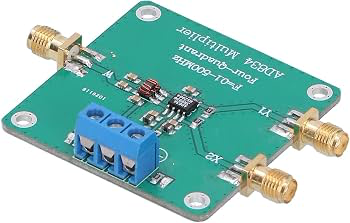
\includegraphics[width=0.7\textwidth]{ad834.png}\\[1cm]
	\caption{AD834 Analog Multiplier Module}
	\label{fig:ad834}
\end{figure}

\subsection{MS-3000 Voltage Controlled Oscillator}

The MS-3000 VCO generates the required local oscillator signal for the frequency mixing operations in the microwave transmission bands.

\begin{table}[H]
	\centering
	\caption{MS-3000 VCO Specifications}
	\label{tab:vco}
	\begin{tabular}{p{5cm} p{5cm}}
		\toprule
		\textbf{Parameter} & \textbf{Value} \\
		\midrule
		Device & MS-3000 \\
		Type & Voltage Controlled Oscillator \\
		Function & Local Oscillator Source \\
		Output & Microwave Frequency Signal \\
		\bottomrule
	\end{tabular}
\end{table}

\begin{figure}[H]
	\centering
	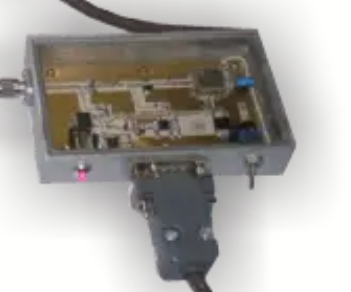
\includegraphics[width=0.7\textwidth]{ms3000.png}\\[1cm]
	\caption{MS-3000 VCO Module}
	\label{fig:vco}
\end{figure}

\subsection{ADE-30 Mixer}

The ADE-30 double-balanced mixer was selected for the lower frequency microwave band as it offers a wide operational range and low conversion loss. It can operate up to 3 GHz and is ideal for applications requiring efficient frequency translation.

\begin{table}[H]
	\centering
	\caption{ADE-30 Mixer Specifications}
	\label{tab:ade31}
	\begin{tabular}{p{5cm} p{5cm}}
		\toprule
		\textbf{Parameter} & \textbf{Value} \\
		\midrule
		Device & ADE-30+ \\
		Frequency Range & 200 MHz -- 3 GHz \\
		LO Drive & +7 dBm \\
		Conversion Loss & 4.5 dB Typical \\
		Type & Passive Double Balanced Mixer \\
		\bottomrule
	\end{tabular}
\end{table}

\begin{figure}[H]
	\centering
	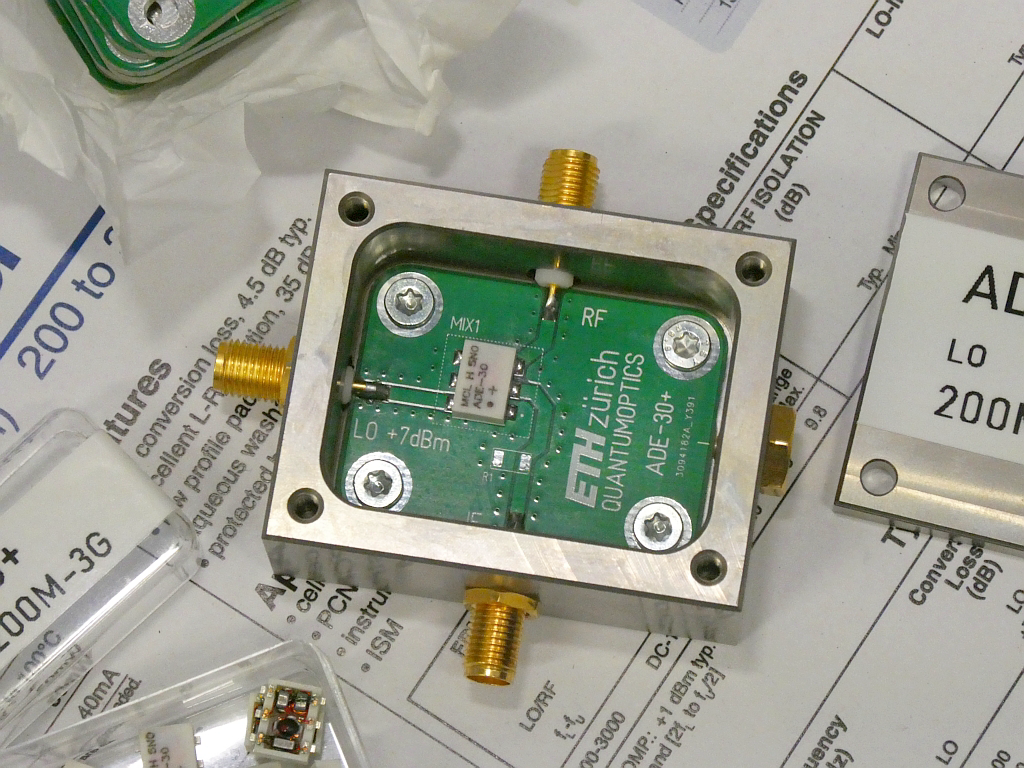
\includegraphics[width=0.7\textwidth]{ade30.png}\\[1cm]
	\caption{ADE-30 Mixer Module}
	\label{fig:ade30}
\end{figure}

\subsection{HMC219 Mixer}

The HMC219 is a GaAs MESFET mixer chosen for operation in the higher microwave frequency range, between 2.5 GHz and 7 GHz. It doesn't require external matching components, simplifying the design, and provides good LO-RF isolation.

\begin{table}[H]
	\centering
	\caption{HMC219 Mixer Specifications}
	\label{tab:hmc219}
	\begin{tabular}{p{5cm} p{5cm}}
		\toprule
		\textbf{Parameter} & \textbf{Value} \\
		\midrule
		Device & HMC219 \\
		Frequency Range & 2.5 GHz -- 7 GHz \\
		IF Range & DC -- 3 GHz \\
		Conversion Loss & 9 dB Typical \\
		Technology & GaAs MESFET \\
		Package & MSOP-8 \\
		\bottomrule
	\end{tabular}
\end{table}

\begin{figure}[H]
	\centering
	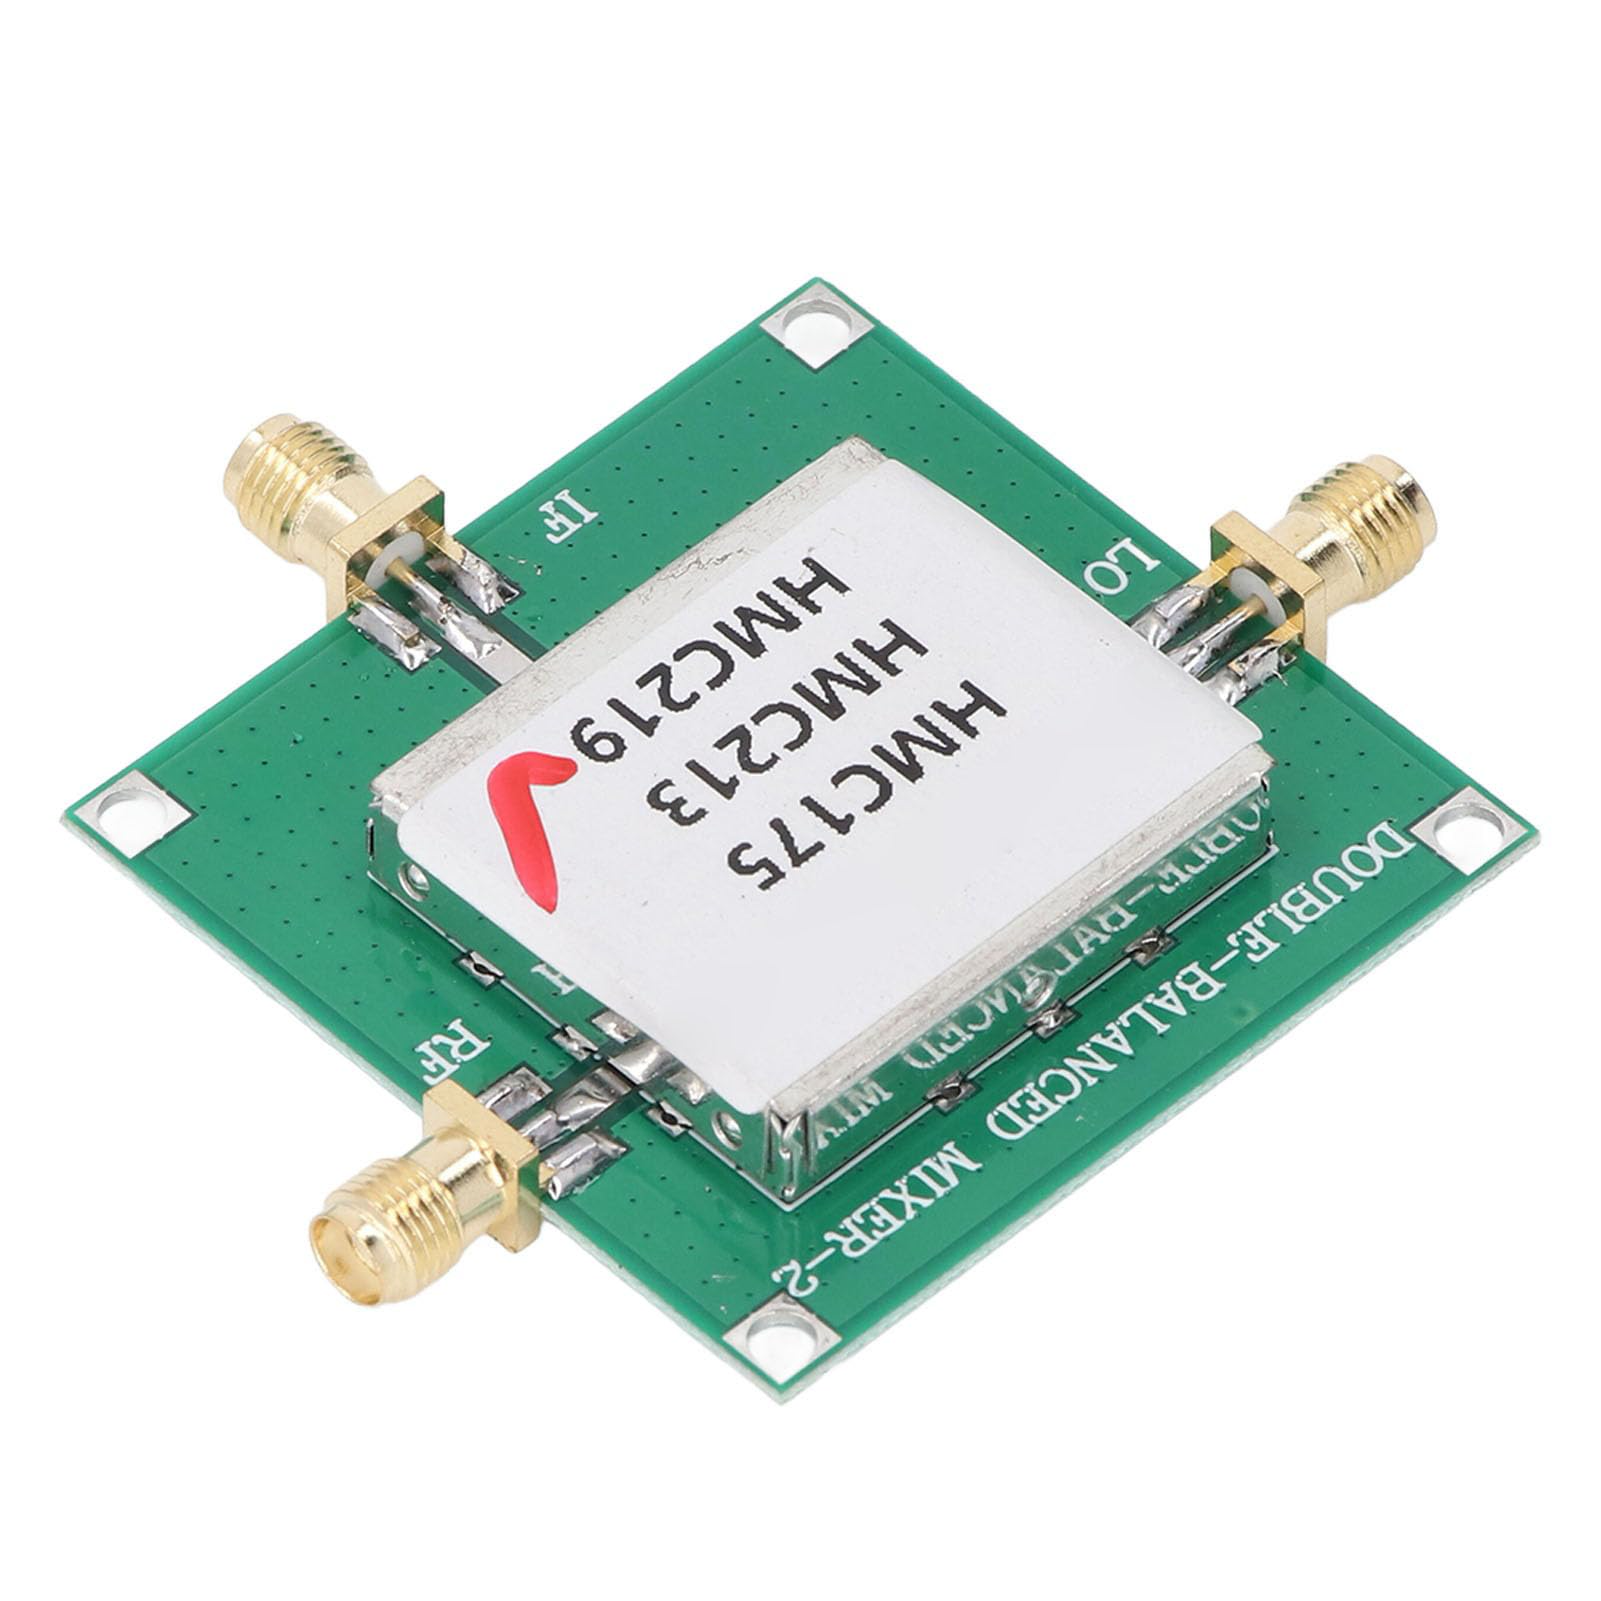
\includegraphics[width=0.7\textwidth]{hmc219.png}\\[1cm]
	\caption{HMC219 Microwave Mixer}
	\label{fig:hmc219}
\end{figure}

\subsection{RF2126 Power Amplifier}

The RF2126 is a power amplifier used to boost the signal power at 2.4 GHz to compensate for the losses in the microwave mixing process. It is specifically designed for ISM band applications.

\begin{table}[H]
	\centering
	\caption{RF2126 Power Amplifier Specifications}
	\label{tab:rf2126}
	\begin{tabular}{p{5cm} p{5cm}}
		\toprule
		\textbf{Parameter} & \textbf{Value} \\
		\midrule
		Device & RF2126 \\
		Technology & GaAs HBT \\
		Operating Range & 1.8 GHz -- 2.5 GHz \\
		Application & ISM Band Amplification \\
		Function & RF Power Amplifier \\
		\bottomrule
	\end{tabular}
\end{table}

\begin{figure}[H]
	\centering
	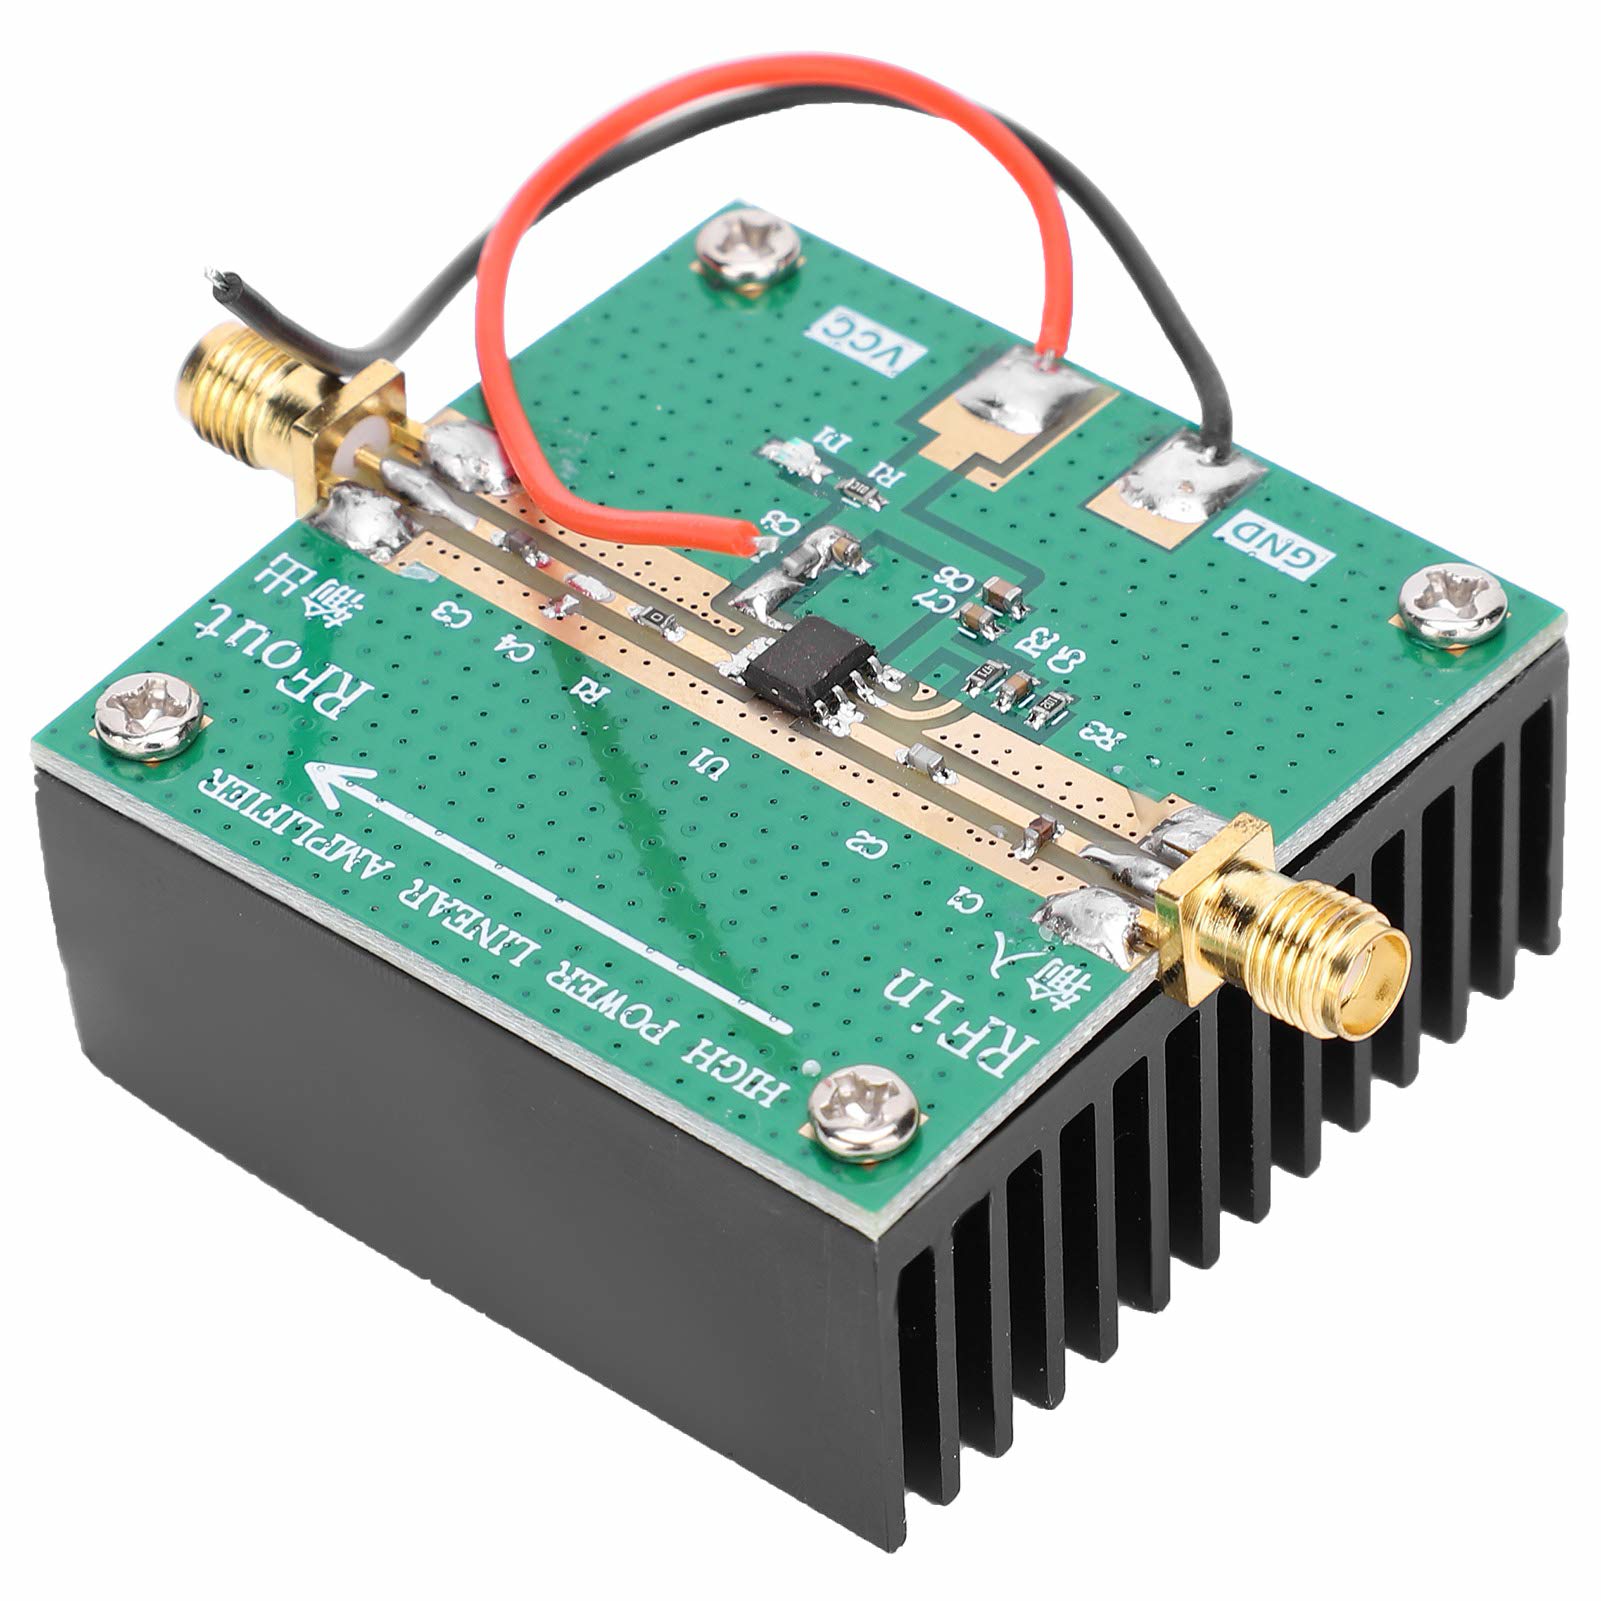
\includegraphics[width=0.7\textwidth]{rf2126.png}\\[1cm]
	\caption{RF2126 Power Amplifier}
	\label{fig:rf2126}
\end{figure}

\subsection{SE5004 Power Amplifier}

The SE5004 amplifier served as the final amplification stage in the upper microwave frequency path, ensuring sufficient transmit power at 5.8 GHz.

\begin{table}[H]
	\centering
	\caption{SE5004 Power Amplifier Specifications}
	\label{tab:se5004}
	\begin{tabular}{p{5cm} p{5cm}}
		\toprule
		\textbf{Parameter} & \textbf{Value} \\
		\midrule
		Device & SE5004 \\
		Function & Power Amplifier \\
		Operating Band & 5.8 GHz \\
		Application & Final RF Gain Stage \\
		\bottomrule
	\end{tabular}
\end{table}

\begin{figure}[H]
	\centering
	\includegraphics[width=0.7\textwidth]{se5004.png}\\[1cm]
	\caption{SE5004 Amplifier Module}
	\label{fig:se5004}
\end{figure}

\subsection{2.4 GHz Directional Antenna}

\begin{table}[H]
	\centering
	\caption{2.4 GHz Directional Antenna Specifications}
	\label{tab:ant24}
	\begin{tabular}{p{5cm} p{5cm}}
		\toprule
		\textbf{Parameter} & \textbf{Value} \\
		\midrule
		Frequency & 2.4 GHz \\
		Gain & 11 $\pm$1 dBi \\
		Impedance & 50 $\Omega$ \\
		VSWR & 1.92:1 \\
		Polarization & Linear Vertical \\
		\bottomrule
	\end{tabular}
\end{table}

\begin{figure}[H]
	\centering
	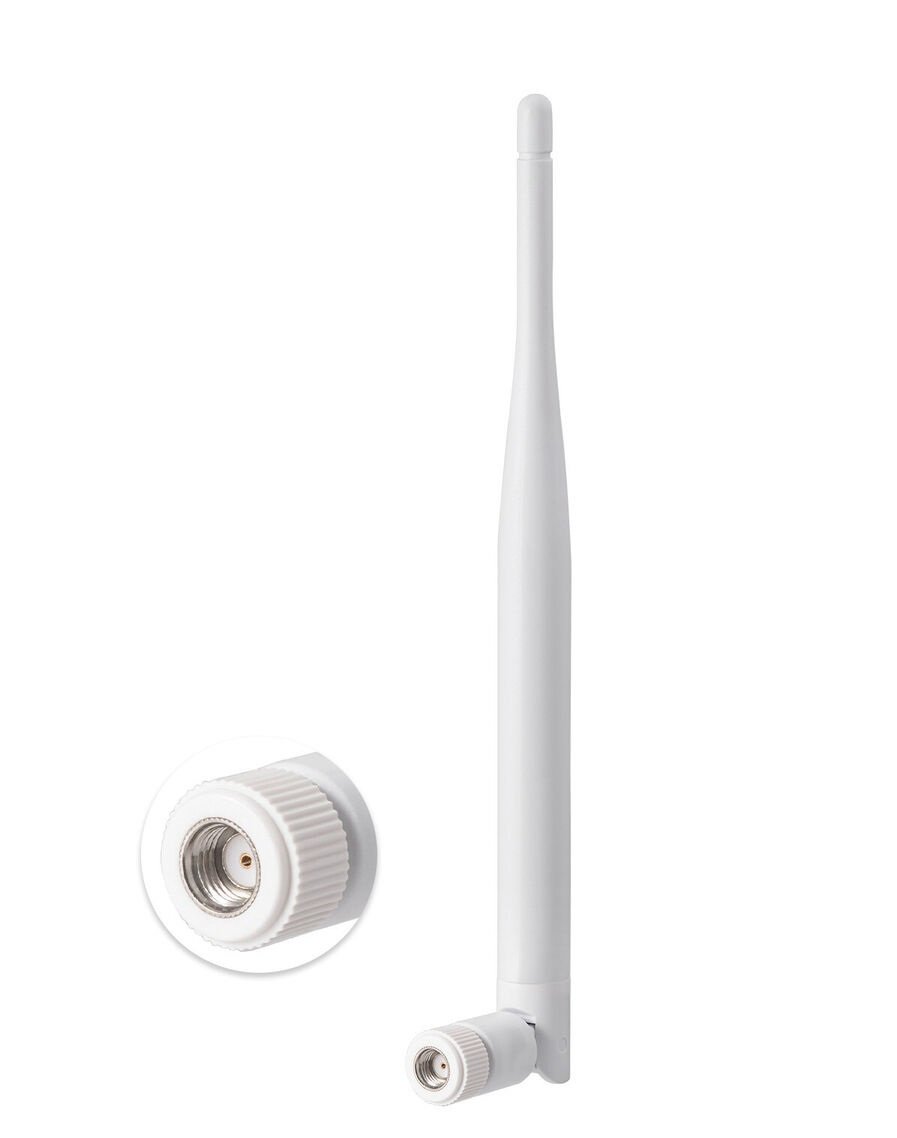
\includegraphics[width=0.7\textwidth]{antenna_2.4ghz.png}\\[1cm]
	\caption{2.4 GHz Directional Antenna}
	\label{fig:ant24}
\end{figure}

\subsection{5.8 GHz Horn Antenna}

A horn antenna was used for the 5.8 GHz path as horn antennas provide high gain, good directivity, and broad bandwidth which are advantageous in microwave frequencies.

\begin{table}[H]
	\centering
	\caption{5.8 GHz Horn Antenna Specifications}
	\label{tab:ant58}
	\begin{tabular}{p{5cm} p{5cm}}
		\toprule
		\textbf{Parameter} & \textbf{Value} \\
		\midrule
		Frequency & 5.8 GHz \\
		Gain & 15 dBi \\
		Type & Horn Antenna \\
		Impedance & 50 $\Omega$ \\
		Polarization & Linear Vertical \\
		\bottomrule
	\end{tabular}
\end{table}

\begin{figure}[H]
	\centering
	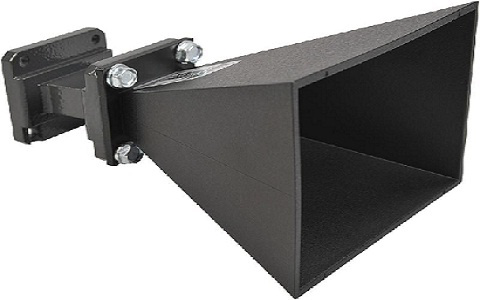
\includegraphics[width=0.7\textwidth]{horn_antenna_5.8ghz.png}\\[1cm]
	\caption{5.8 GHz Horn Antenna}
	\label{fig:horn_ant}
\end{figure}

\subsection{Digital Oscilloscope}

The digital oscilloscope was crucial throughout the entire hardware development process for monitoring signals in the time domain and verifying proper functionality. It was extensively used for observing the generated noise signal, the output of the coupling capacitor, the modulation signal, the carrier signal, bias voltages, and any signal distortions or clipping. Digital oscilloscopes are indispensable tools in RF laboratories due to their ability to provide time-based analysis that cannot be fully achieved by frequency-domain instruments alone.

\begin{table}[H]
	\centering
	\caption{Digital Oscilloscope Specifications}
	\label{tab:oscilloscope}
	\begin{tabular}{p{5cm} p{5cm}}
		\toprule
		\textbf{Parameter} & \textbf{Typical Value} \\
		\midrule
		Bandwidth & 100 MHz or higher \\
		Sampling Rate & 1 GS/s \\
		Channels & 2 or 4 \\
		Input Impedance & 1 M$\Omega$ \\
		\bottomrule
	\end{tabular}
\end{table}

\begin{figure}[H]
	\centering
	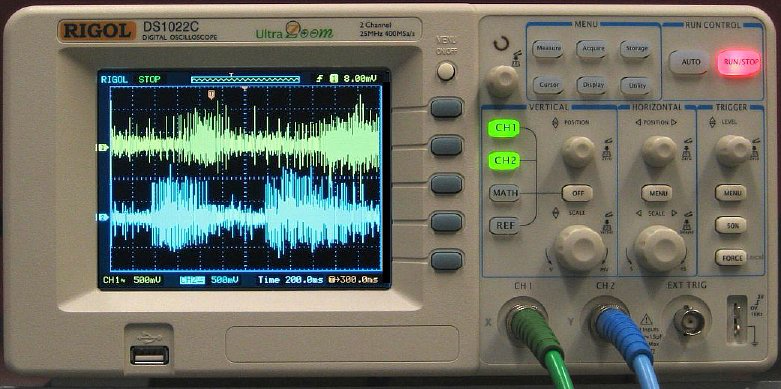
\includegraphics[width=0.7\textwidth]{oscilloscope.png}\\[1cm]
	\caption{Digital Oscilloscope Used During Testing}
	\label{fig:oscilloscope}
\end{figure}

\subsection{Spectrum Analyzer}

The spectrum analyzer was the primary instrument employed for all frequency domain measurements. Unlike an oscilloscope which plots amplitude versus time, a spectrum analyzer displays signal power versus frequency, making it essential for identifying the signal's spectral characteristics. The instrument was utilized for checking frequency accuracy, identifying harmonic components, measuring occupied bandwidth, detecting unwanted spurious signals, analyzing the spectra of mixer outputs, and verifying amplifier performance. The spectrum analyzer is considered one of the most important test instruments in an RF and microwave laboratory.

\begin{table}[H]
	\centering
	\caption{Spectrum Analyzer Specifications}
	\label{tab:spectrum}
	\begin{tabular}{p{5cm} p{5cm}}
		\toprule
		\textbf{Parameter} & \textbf{Typical Value} \\
		\midrule
		Frequency Range & 9 kHz -- 3 GHz or higher \\
		Resolution Bandwidth & 1 Hz -- 1 MHz \\
		Display & Frequency vs. Power \\
		Application & Spectral Analysis \\
		\bottomrule
	\end{tabular}
\end{table}

\begin{figure}[H]
	\centering
	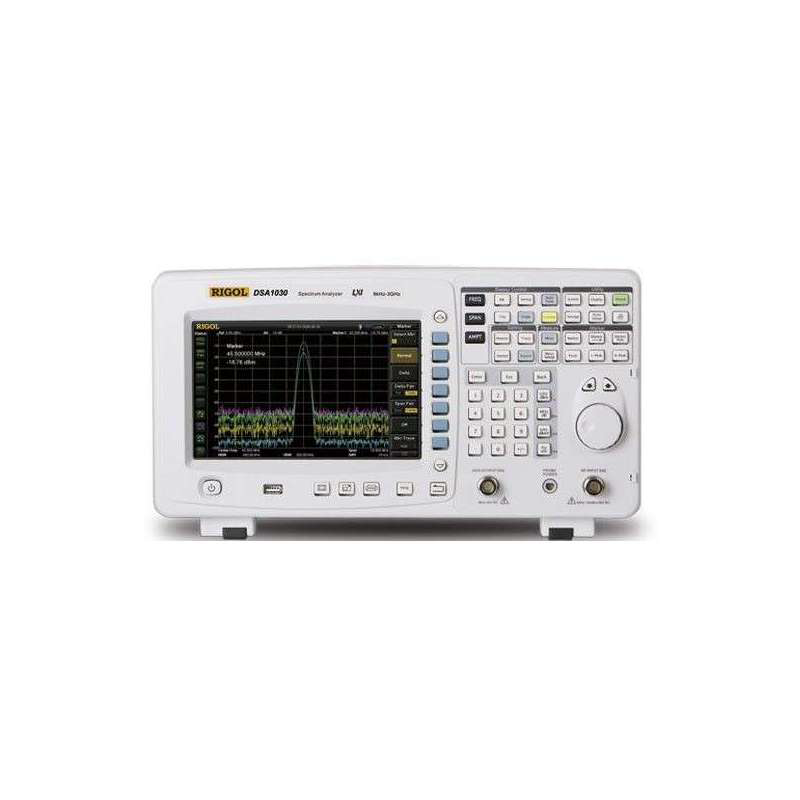
\includegraphics[width=0.7\textwidth]{spectrum_analyzer.png}\\[1cm]
	\caption{Spectrum Analyzer}
	\label{fig:spectrum}
\end{figure}
	\chapter{Results and Discussion}
	
	\chapter{Conclusion and Future Work}
	
\end{document}